%*******************************************************************
%                      Proyecto de Título                          *
% Ingeniería Civil en Informática - Universidad Austral de Chile   *
% Autor: Miguel Esteban Orellana Concha 				           *
%        es.orellana@gmail.com				                       * 
% Tesis: Gestión de tickets de espera para centros de atención,    *
%        utilizando notificaciones Push Android                    *
%        Enero de 2015 - Valdivia                                  *   
% Patrocinante: Jorge Morales 					                   *  
% Co patrocinante: María Eliana de la Maza                         *                                       
%*******************************************************************

\documentclass[12pt]{article} 
\usepackage[papersize={216mm,330mm},left=4cm,right=2.5cm,top=1.88cm,bottom=3cm]{geometry} 
\usepackage[spanish]{babel}
\usepackage[utf8]{inputenc}
\usepackage{graphicx}
\usepackage{xcolor}
\usepackage{xcolor,colortbl}
\usepackage[pdftex,
			colorlinks=true,
			linkcolor=black,
			citecolor=black,
			filecolor=black,
			urlcolor=black,
			hyperfootnotes=false,
            pdfauthor={Miguel Esteban Orellana Concha},
            pdftitle={Gestión de tickets de espera para centros de atención, utilizando notificaciones Push Android},
            pdfsubject={Tesis},
            pdfkeywords={6LoWPAN, BMS, IPv6, IoT, WSN},
            pdfproducer={Latex with hyperref},
            pdfcreator={pdflatex}]{hyperref}
\usepackage{url}
\usepackage[bottom]{footmisc}
\usepackage{float}
\usepackage{nonfloat}
\usepackage{setspace}
\usepackage[titles]{tocloft}
\usepackage{lipsum,titletoc}
\usepackage{tocloft}
\usepackage{amsmath}
\usepackage[T1]{fontenc} % Times New Roman
\usepackage{txfonts}
\usepackage{sectsty}
\usepackage[labelsep=period]{caption}
\usepackage{multirow}
\usepackage{fancyhdr}


\pagestyle{fancy}
\fancyhead{}
\fancyfoot[CE,CO]{\thepage}
\renewcommand{\headrulewidth}{0.0pt}
\renewcommand{\footrulewidth}{0.0pt}
\usepackage[figuresright]{rotating} 
\renewcommand{\baselinestretch}{1.5}
\pretolerance=10000
\tolerance=10000

\setcounter{secnumdepth}{5}
\setcounter{tocdepth}{5}

\newcommand{\myparagraph}[1]{\paragraph{#1}\mbox{}\\}

\sectionfont{\fontsize{14}{14}\selectfont}
\subsectionfont{\fontsize{14}{14}\selectfont}

\newcommand{\blockline}{\par\noindent\hspace{-0.05\textwidth}%
    \textcolor{black}{\rule{1.05\textwidth}{0.35mm}}\par\nobreak}
       
    
\begin{document}





%##########################################################
%PORTADA

\thispagestyle{empty}
\setcounter{page}{1}
\begin{spacing}{1.0}

\begin{center}

\includegraphics[width=2.65cm, height=3.18cm]{images/portada/escudo.png}\\
\vspace{0.5cm}

\includegraphics[width=13.02cm, height=1.23cm]{images/portada/uach.png}\\
\vspace{-0.4cm}
\blockline
\vspace{0.2cm}
{\fontsize{24}{24}\selectfont Facultad de Ciencias de la Ingeniería}\\[0.1cm]
{\fontsize{18}{18}\selectfont Escuela de Ingeniería Civil en Informática}\\
\end{center}

\vspace{2.0cm}

\begin{center}
	%{\fontsize{18}{18}\selectfont \bf PROYECTO DE TÍTULO}\\[0.5cm]
	{\fontsize{18}{18}\selectfont \bf GESTIÓN DE TICKETS DE ESPERA PARA}\\[0.2cm]
	{\fontsize{18}{18}\selectfont \bf CENTROS DE ATENCIÓN, UTILIZANDO}\\[0.2cm]
	{\fontsize{18}{18}\selectfont \bf NOTIFICACIONES PUSH ANDROID.}\\[0.2cm]   
	
\end{center}

\vspace{2.0cm}

\begin{flushright} \small
{\fontsize{10}{10}\selectfont Proyecto para optar al título de}  \textcolor{white}{.}\\
{\fontsize{10}{10}\selectfont \bf Ingeniero Civil en Informática} 
\end{flushright}

\vspace{1.0cm}

\begin{flushleft} \small
\hspace{-1cm}{\fontsize{11}{11}\selectfont PROFESOR PATROCINANTE:}\\
\hspace{-1cm}{\fontsize{11}{11}\selectfont JORGE ANTONIO MORALES VILUGRÓN}\\
\hspace{-1cm}{\fontsize{11}{11}\selectfont INGENIERO ELECTRÓNICO}\\
\hspace{-1cm}{\fontsize{11}{11}\selectfont M.B.A., D.E.A. MICROCONTROLADORES}\\
\vspace{0.5cm}
\hspace{-1cm}{\fontsize{11}{11}\selectfont PROFESOR CO-PATROCINANTE:}\\
\hspace{-1cm}{\fontsize{11}{11}\selectfont MARÍA ELIANA DE LA MAZA WERNER}\\
\hspace{-1cm}{\fontsize{11}{11}\selectfont INGENIERO CIVIL EN INFORMÁTICA}\\
\hspace{-1cm}{\fontsize{11}{11}\selectfont MAGÍSTER EN INFORMÁTICA EDUCATIVA}\\

\vspace{0.5cm}
\hspace{-1cm}{\fontsize{11}{11}\selectfont PROFESOR INFORMANTE:}\\
\hspace{-1cm}{\fontsize{11}{11}\selectfont N.N.}\\
\hspace{-1cm}{\fontsize{11}{11}\selectfont N.N.}\\
\end{flushleft}

\vspace{1.0cm}

\begin{center}
{\fontsize{16}{16}\selectfont \bf MIGUEL ESTEBAN ORELLANA CONCHA}\\
\vspace{0.4cm}
{\fontsize{10}{10}\selectfont VALDIVIA - CHILE}\\
{\fontsize{10}{10}\selectfont 2015}\\
\end{center}

\end{spacing}

%##########################################################

\newpage

\newgeometry{left=4cm,right=2.5cm,top=4cm,bottom=3cm} % Márgenes documento
\renewcommand{\tablename}{Tabla}

% Formato de indices
\renewcommand\contentsname{}
\renewcommand\listfigurename{}
\renewcommand\listtablename{}

\setlength{\cftbeforesecskip}{0ex}
\titlecontents{section} 
[2.3em]                 
{\rmfamily}            
{ \contentslabel{1.3em}} 
{\hspace*{-1.0em}}
{\titlerule*[0.7pc]{.}\contentspage}

\setlength{\cftsecnumwidth}{0.8em}  % espacio en ToC
\setlength{\cftsubsecnumwidth}{1.8em}
\setlength{\cftsubsubsecnumwidth}{2.5em}
\setlength{\cftparanumwidth}{3em}
\setlength{\cftsubsecindent}{2.0em}
\setlength{\cftsubsubsecindent}{3.0em}
\setlength{\cftparaindent}{4.0em}
\setlength{\cftfignumwidth}{1.5em}  % espacio entre números con LoF
\setlength{\cfttabnumwidth}{1.5em}  % espacio entre números con LoT


\setlength{\parindent}{0pt} % sangrías


%----------------------------------------------------------
% NOTAS

%----------------------------------------------------------
% AGRADECIMIENTOS
\thispagestyle{empty}
\begin{center}
{\fontsize{14}{14}\selectfont \bf AGRADECIMIENTOS}\\
\end{center}

%En primer lugar quiero agradecer a la mujer más importante de mi  vida,  la que se desveló más de una noche  para cuidar de mi salud, la que muchas veces pasó hambre para que yo me alimentara bien, la mujer que me enseñó a levantarme todas las veces que sean necesarias para lograr mis objetivos, estoy hablando de mi madre, María Napoli, sin ella yo no  estaría escribiendo este documento, gran parte de mis logros se los debo a ella. Agradezco a mi hermano,  que a pesar de todo lo ocurrido el me enseñó que en la vida hay que ser valiente, él me enseñó a que pase lo que pase, nunca agachar la cabeza. También quiero agradecer a mi hermana Mavian por su incondicional apoyo.
\\

Quiero agradecer de forma especial a mis dos grandes amigos que siempre me apoyaron y creyeron en mí, Tere y Colin, sin ustedes  no me hubiera levantado tan fácilmente, ustedes han  bailado conmigo bajo la lluvia, y no lo digo tan literalmente.\\

Agradezco a mi amiga Niza, que a pesar de que no compartamos las mismas ideologías, me ayudó mucho en mi proceso formativo \\

Agradezco a mi tía nana, que al momento de pedirle ayuda, no dudó en ofrecerme más de lo que yo le pedí.\\

Agradezco a mi segundo hogar, el Trensito,  con ustedes conviví más de cinco años, y fue genial sentir el compañerismo que existe ahí.
\\

César Soto, a pesar de que nos conocimos en un ambiente laboral, te convertiste en un gran amigo y siempre estuviste dispuesto a ayudarme, te lo agradezco de todo corazón, no muchas personas con como tú.\\



Con respecto a los profesores de la universidad, quiero agradecer al profesor Mauricio, quien se convirtió en mi profesor guía durante la última etapa de mi formación profesional y a la profesora María Eliana, quien siempre me brindó su ayuda, a pesar de que estuviera ocupada. 
 \\

 
Para último quiero agradecer a todas las personas que no he podido nombrar, pero que de alguna u otra  manera me han ayudado  a finalizar este proceso, GRACIAS A TODOS!!!.


 
 
 
 
 

\newpage

\setcounter{page}{1}
\renewcommand{\thepage}{\roman{page}} 

%##########################################################
%INDICES

%----------------------------------------------------------
% Indice de contenidos
\begin{center}
{\fontsize{14}{14}\selectfont \bf ÍNDICE}\\
\end{center}
\phantomsection
\addcontentsline{toc}{section}{ÍNDICE}
\vspace{-1.0cm}
\begin{spacing}{1.2}
{\fontsize{10}{10}\selectfont \tableofcontents}
\end{spacing}


\newpage

%----------------------------------------------------------
% Indice de tablas - LoT
\begin{center}
{\fontsize{14}{14}\selectfont \bf ÍNDICE DE TABLAS}\\
\end{center}
\phantomsection
\addcontentsline{toc}{section}{ÍNDICE DE TABLAS}

\begin{flushright} \small
TABLA \hspace{11.6cm} PÁGINA\\
\end{flushright}

\vspace{-1.0cm}

\begin{spacing}{1.2}
{\fontsize{10}{10}\selectfont \listoftables}
\end{spacing}

\newpage

%----------------------------------------------------------
% Indice de figuras - LoF
\begin{center}
{\fontsize{14}{14}\selectfont \bf ÍNDICE DE FIGURAS}\\
\end{center}
\phantomsection
\addcontentsline{toc}{section}{ÍNDICE DE FIGURAS}


\begin{flushright} \small
FIGURA \hspace{11.45cm} PÁGINA\\
\end{flushright}

\vspace{-1.0cm}

\begin{spacing}{1.2}
{\fontsize{10}{10}\selectfont \listoffigures}
\end{spacing}

\newpage


%----------------------------------------------------------
% RESUMEN
\begin{center}
{\fontsize{14}{14}\selectfont \bf RESUMEN}\\
\end{center}
\phantomsection
\addcontentsline{toc}{section}{RESUMEN}

Este Proyecto de Titulación pretende mejorar el proceso de atención de los usuarios que acuden a una oficina para realizar un trámite, de tal modo de optimizar el tiempo de espera en las interminables filas de este servicio.\\

El objetivo general del proyecto, es el desarrollo de un sistema capaz de solicitar un número de atención a través de una aplicación para Smartphones con Sistema Operativo Android, y hacer el seguimiento vía Notificaciones Push de los tickets de espera para personas que estén en algún centro de atención, con el objeto de optimizar los tiempos de espera. Es decir, los usuarios podrían salir del recinto y realizar otros trámites y con ello hacer más eficiente su tiempo.\\

Actualmente, las filas de espera en los diferentes centros de atención cuentan con un ticket manual y los clientes deben permanecer al interior del recinto. Las nuevas tecnologías emergentes y de uso masivo, como los Smartphones, representan una oportunidad para incorporar tecnología a éste proceso de atención. Particularmente el diseño de un tablero que envíe notificaciones del estado de la fila al Smartphone del cliente. Ésta información  es almacenada y es la base para generar diversos reportes y con ellos mejorar la gestión de los servicios.\\

En este proyecto se propone una solución utilizando tecnología de vanguardia, que es la plataforma Web y la utilización de Smartphones con Sistema Android para el aprovechamiento de la información obtenida y seguimiento de las colas de espera.\\

Finalmente, se define la mejor forma de implementar este sistema acompañada de una validación de esta implementación.\\




\newpage

%----------------------------------------------------------
% ABSTRACT
\begin{center}
{\fontsize{14}{14}\selectfont \bf ABSTRACT}\\
\end{center}
\phantomsection
\addcontentsline{toc}{section}{ABSTRACT}



"The Austral University of Chile is an accredited institution that trains professionals and graduates of undergraduate and postgraduate, with a stamp characterized by academic excellence, commitment to freedom and the socio cultural environment, respect for diversity, social responsibility, among others "\hspace{0.2cm} \cite{MOD07}.Compliance with these definitions in the \textit{educational model and curriculum approach}, require, among others, internal processes of the organization to support educational management, particularly, undergraduate. One of the most important features in this area, It’s the management curriculum career projects. Therefore it is very important to know the curricular history of each career, need that giving rise to this project.
\\

The aim of this thesis project is to design and develop a prototype of web platform to manage curricular history of every UACh‘s career , which will allow to a different units of the university have better curricular information about the careers and thus facilitate the work done every day.
\\

The web system is developed for the Autral University of Chile, it’s for that reason that the thesis student must adapt to technologies that the university uses, therefore the solution will be developed in the following technologies: Microsoft Visual Studio 2013, Microsoft SQL server 2008 (only in development environment, once the project is completed will be migrated to Sybase, which is the database engine used by the university), Visual basic and server language, JavaScript, cSS3, HTML5 and GitHub as manager versions.
\\

The web system will benefits the departement area undergraduate of the university n which they are constantly manipulating curricular careers information, these department are: Department of Quality Assurance and Curriculum Innovation (Dacic), Department of Student Academic Registry and Admission and Registration Department, also it will benefit the school itself, as it will allow them to have curricular historical information.
\\

The advantages of having a web platform that stores career’s historical data of carrera is to reduce the work that these departments have when require some curricular information.

\newpage

%##########################################################
% CUERPO DEL DOCUMENTO

\setcounter{page}{1}
\renewcommand{\thepage}{\arabic{page}}

%----------------------------------------------------------
%----------------------------------------------------------
\section{INTRODUCCIÓN}
%----------------------------------------------------------
%----------------------------------------------------------
% INTRODUCCIÓN
	"Durante la última década, las universidades pertenecientes al Consejo de Rectores de Universidades chilenas (CRUCH) 
	han promovido diversas iniciativas de Innovación Curricular" \cite{INN11}. Es por ello que la Universidad Austral de 
	Chile ya ha empezado con el proceso de innovación curricular para que gradualmente abarque todas sus carreras.
	\\
	
	Uno de los principales problemas relacionados con el proceso de calidad e innovación curricular es que la Universidad 
	Austral de Chile almacena toda la información referente al historial curricular de cada carrera en distintos medios 
	de almacenamiento (incluyendo el papel), distintos  formatos, y en varias unidades de la organización, lo que 
	dificulta la generación de informes que apoyen procesos estratégicos de seguimiento y auto-evaluación.
	\\
	
	Este proyecto surge como una iniciativa del Dr. Mauricio Ruiz-Tagle quien observó las falencias que tienen los 
	departamentos ya indicados al momento de gestionar documentos relacionados con la innovación curricular.  
	De acuerdo a lo mencionado anteriormente, se pretende crear una plataforma web, que permita gestionar el historial 
	curricular de cada carrera de la universidad, la cual permitirá a distintas Unidades de la universidad tener una 
	mejor información  de las carreras y así facilitar el trabajo que día a día realizan.
	\\
	
	La información obtenida por esta plataforma servirá de apoyo para la gestión curricular por parte de los distintos departamentos que integran la Dirección de Estudios de Pregrado, ya que se contará con todo lo necesario para gestionar los cambios curriculares de los planes de estudio.

	\subsection{Definición del Proyecto}
	
	\subsubsection{Objetivo general}
	
	Diseñar y construir  un prototipo de una plataforma web que apoye al monitoreo curricular de pregrado \\
	\vspace{-0.4cm}
	
	\subsubsection{Objetivos específicos}
	
	\begin{itemize}
		\item Conocer cómo los departamentos que integran la Dirección de Estudios de Pregrado (DEP) administran
		la información referente a los planes de estudios.
		\item  Definir requerimientos del sistema, describiendo sus funcionalidades y separar en módulos la aplicación.
		\item Diseñar e implementar el módulo necesario que permita gestionar el historial curricular de una carrera en particular.
		\item Diseñar e implementar el módulo necesario que permita gestionar el historial de la escuela de una carrera en particular.
		\item Realizar pruebas de validación de los requisitos y estabilidad del prototipo de plataforma web.
	\end{itemize}
	\subsection{Nivel actual}
	
		Como ya se ha mencionado anteriormente el presente proyecto pretende aportar a los procesos curriculares de la Universidad Austral de Chile, es por esto mismo que es necesario entender los procesos que realizan los departamentos involucrados.
		\\
		
		En la Figura \ref{Figura1} se puede apreciar como se estructuran los departamentos de Vicerrectoría. A partir de este diagrama se explicarán las principales funciones y procesos de los Departamentos de Estudios de Pregrado, los cuales son: Departamento de Aseguramiento de la Calidad de la Docencia e Innovación Curricular, Departamento de Admisión y Matricula y Departamento de Registro Académico Estudiantil.
	
		\begin{figure}[h]
			\centering
			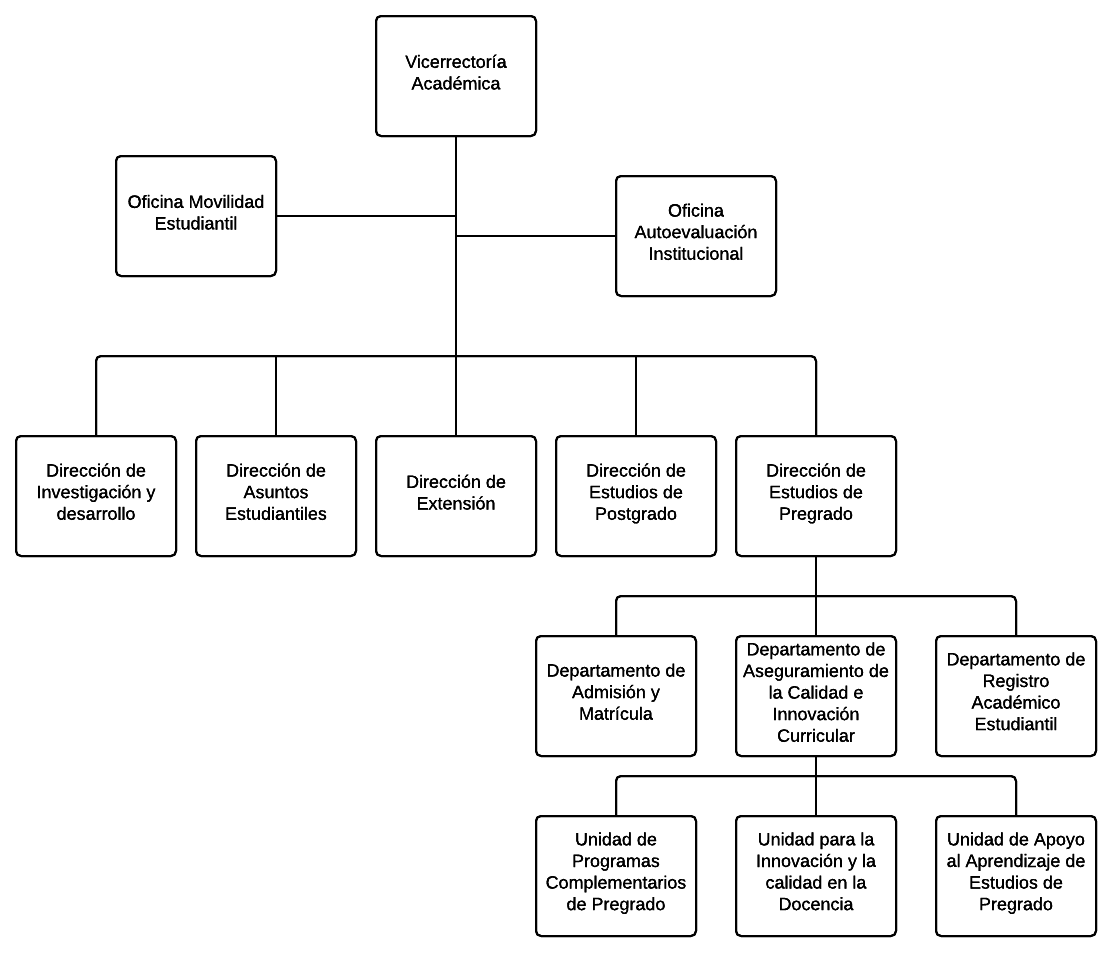
\includegraphics[width=1\textwidth]{images/Capitulo_1/Organigrama.png}
			\caption[Organigrama Vicerrectoría y DACIC]{Organigrama Vicerrectoría y DACIC \footnote{}}
			\label{Figura1}
		\end{figure}
		\footnotetext{Elaboración propia.}
		
		\subsubsection{Departamento de Aseguramiento de la Calidad e Innovación Curricular (DACIC)}
		
		
		En este departamento nace la idea de desarrollar un sistema que apoye a los procesos curriculares. Su principal objetivo es ``propender al fortalecimiento de la calidad de los aprendizajes de los estudiantes de la UACh a través del apoyo a las y Docentes en el diseño de situaciones de enseñanza/aprendizaje orientadas a la obtención de resultados efectivos y el asesoramiento a las unidades académicas respectivas en el desarrollo de innovaciones curriculares."\cite{Dac15}
		\\
		
		El departamento está conformado por cuatro Unidades:
			\begin{itemize}
				\item Unidad de Apoyo al Desarrollo de la Docencia de Pregrado
				\item Unidad de Apoyo al Desarrollo y la Innovación Curricular en Pregrado
				\item Unidad de Apoyo al Aprendizaje del Estudiante de Pregrado 	
				\item  Unidad de Programas Complementarios
			\end{itemize}
		
		Sin embargo el proyecto beneficiará directamente  a la Unidad de Apoyo al Desarrollo y la Innovación Curricular en Pregrado, por lo que se dará mas detalles de esta Unidad a continuación.
		
		
		\myparagraph{Apoyo al Desarrollo y la Innovación Curricular en Pregrado}
		
		Unidad encargada de apoyar en el ámbito ``técnico-curricular a las escuelas de Pregrado en sus proyectos de innovación curricular, tanto en carreras profesionales como técnicas, en el contexto del Modelo Educativo y Enfoque Curricular de la Universidad."\cite{Dac15}
		\subsubsection{Departamento de Admisión y Matrícula}
		
		Como su nombre lo indica, este departamento esta presente cuando el alumno ingresa a la Universidad Austral de Chile, en cualquiera de las siguientes modalidades:
			\begin{itemize}
				\item Sistema regular, común a toda la Educación Superior adscrita al Consejo de Rectores de las Universidades Chilenas.
				\item Sistema de Ingreso Especial, propio de la Universidad.
			\end{itemize}
			
			\myparagraph{Servicios estudiantiles} 
		
			\begin{itemize}
				\item 	`` El Departamento de Admisión y Matrícula es la Unidad encargada de otorgar las certificaciones de Alumno Regular a todos los estudiantes de la Universidad, que cumplan con los requisitos para la de emisión de dichos documentos."\cite{Dep15}
				\item Gestiona  la construcción y entrega de las Credenciales Universitarias.
			\end{itemize}
			
		
		
		
		\subsubsection{Departamento de Registro Académico Estudiantil}
		
		Este departamento depende directamente de la Dirección de Estudios de Pregrado de la Vicerrectoría Académica, esta a cargo de la Sra. María Cristina Barriga Ramírez. Entre sus funciones se destaca ``el seguimiento académico del estudiante de pregrado, postítulo y postgrado desde su primera matrícula hasta su egreso y posterior titulación y/o graduación y el permanente apoyo a la labor administrativa que realizan Directores de Escuela, Directores de Unidades Académicas y Profesores en general"\cite{Dir15}.
		
		
		
		
		
		
		\myparagraph{Procesos:}
		
		Esta Unidad  controla la información académica - administrativa, prepara y supervisa los siguientes procesos:
		\begin{itemize}
			\item Peticiones de asignaturas que realizan las Escuelas.
			\item Oferta de asignaturas de las Unidades Académicas.
			\item Inscripción de asignaturas de los estudiantes.
			\item Ingreso de las calificaciones por parte de los profesores.
			\item Modificaciones curriculares de los planes de estudios, de acuerdo  a lo aprobado por la Dirección de Estudios de Pregrado.
			
		\end{itemize}
		
		
		Una vez nombrado los diferentes procesos que controla este departamento, se procederá a explicar los dos  principales procesos que están directamente relacionado con el sistema, los cuales son: Creación de nuevas Carreras y  Modificaciones curriculares de los planes de estudios, de acuerdo  a lo aprobado por la Dirección de Estudios de Pregrado.
		
		\myparagraph{Creación de nuevas Carreras}
		
		En el diagrama de procesos que se muestra en la Figura \ref{Figura2} describe la secuencia básica que se lleva a cabo para la creación de nuevas carreras en la Universidad Austral de Chile.
		\begin{figure}[H]
			\centering
			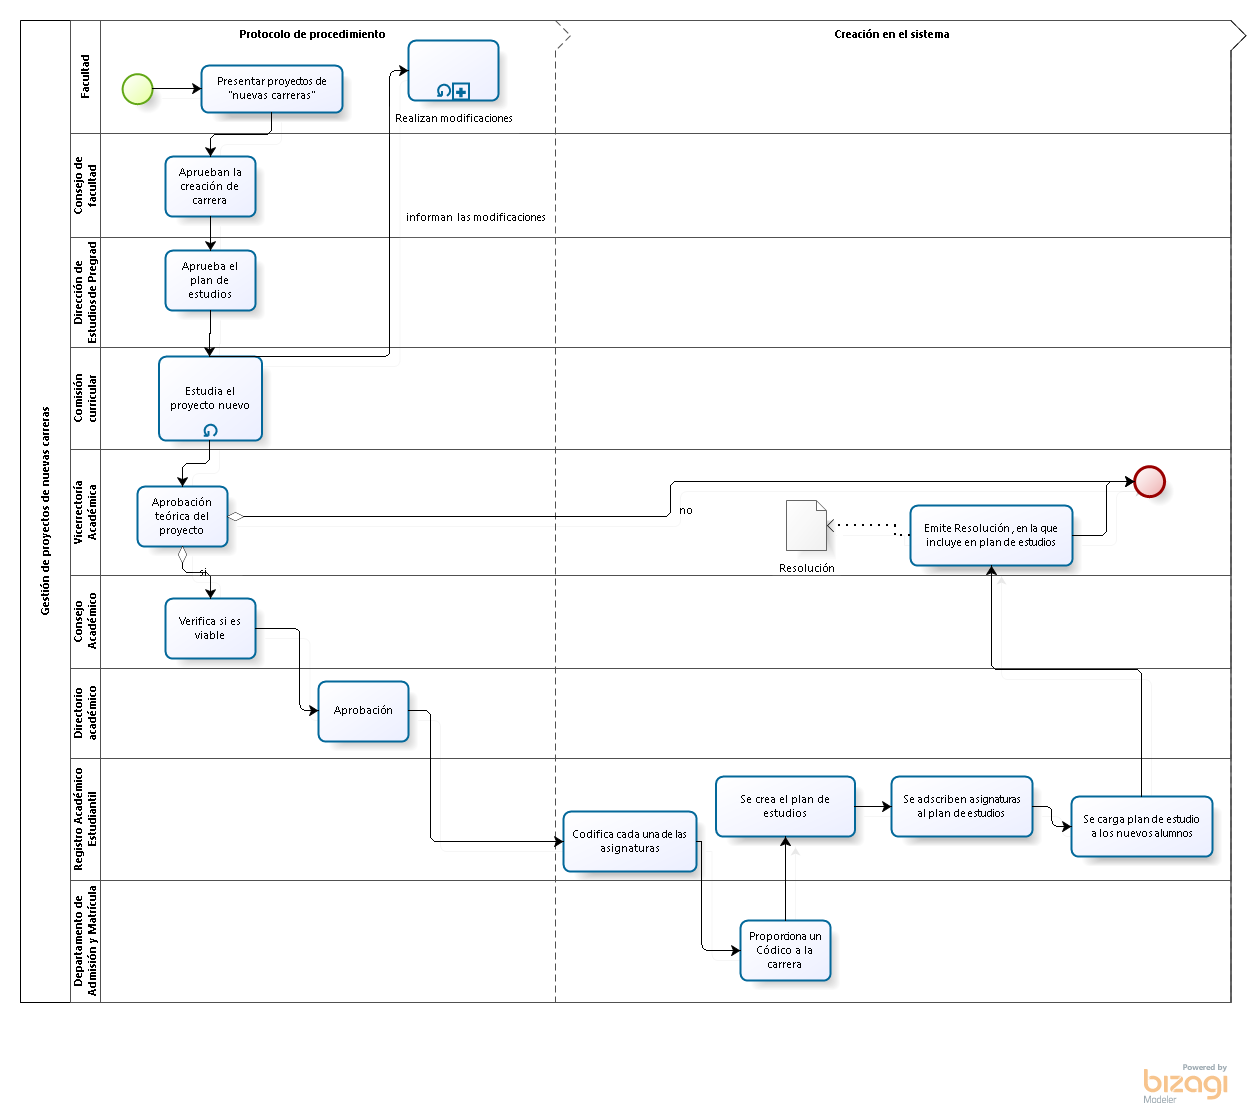
\includegraphics[width=0.9\textwidth]{images/Capitulo_1/Procesos_Registro_academico.png}
			\caption[Proceso de presentación de nuevos proyectos]{Proceso de presentación de nuevos proyectos \footnote{}}
			\label{Figura2}
		\end{figure}
		\footnotetext{Elaboración propia.}	
		
		Las fechas para la presentación de nuevos proyectos o innovaciones curriculares, se estipulan en el Decreto de Rectoría  que promulga el Calendario Académico cada año. Para el año 2015 se especifica:
		
		\begin{itemize}
			\item 30 de abril, último día para presentar en la Vicerrectoría Académica, los proyectos de nuevas carreras.
			\item 30 de junio, último día para que las facultades y sedes presenten proyectos de Innovación Curricular de las carreras a la Vicerrectoría Académica.
		\end{itemize}
		
		
		Una vez aprobado una nueva carrera o la innovación curricular por parte de la Vicerrectoría Académica, los pasos administrativos, son los que se indican a continuación:
		
		
		
		
		\begin{enumerate}
			
			
			\item Se codifica cada una de las asignaturas, asociándose a una Unidad Académica especifica. La Unidad Académica es la que le asigna la sigla, en letras y la numeración es un correlativo que se utiliza para la identificación de la asignatura. Ejemplo: CAEV222-14.
			\\
			CAEV = Ciencias Ambientales y evolutivas (Unidad Académica)
			\\
			222   = Numeración asignada para identificarla dentro de la misma unidad.
			\\
			-14    = año de creación (2014)
			
			\item El Departamento de Admisión y Matrícula proporciona  un código a la carrera. Ejemplo 1826, Escuela de Psicología (valdivia).
			
			\item Una vez que las carreras estén creadas y las asignaturas asociadas a una unidad académica, el Departamento de Registro Académico Estudiantil crea el plan de estudios (ver Figura \ref{Figura2}) con la descripción del propio plan:Nombre de bachillerato,Duración, Año de creación,e etc.
			
			\item El proceso final para la creación de una carrera, es cargar  las asignaturas al plan previamente creado, los pasos son los siguientes:
			\begin{enumerate}
				\item Se ingresa una a una las asignaturas previamente creadas.
				\item Se asocia a un semestre en particular.
			\end{enumerate}
		\end{enumerate}
		\newpage
		\myparagraph{Modificaciones Curriculares Mayores y/o Menores}
		
		Tanto la creación de nuevas carreras como todo lo que tiene que ver con modificaciones con respecto al plan de estudio, son proceso que ve el DACIC, específicamente el sub-departamento de Unidad de Apoyo al Desarrollo y la Innovación Curricular en Pregrado, en conjunto con Registro Académico Estudiantil.
		\\
		
		La Figura \ref{Figura2} muestra los procesos administrativos que realiza Registro Académico Estudiantil, a continuación se explicará con mayor detalle.
		El proceso de modificación del plan de estudio comienza con la iniciativa de una escuela, la cual se reúne previamente con Registro Académico Estudiantil, con el objetivo  de identificar quiénes son los afectados por los cambios (número de alumnos, año de ingreso, plan de Estudios, etc.). Una vez concretada esta reunión, la escuela se encuentra en condiciones de formalizar la petición, la cual es enviada a Dirección de Pregrado con la intención de que sea evaluada. En caso de que la petición sea viable, Dirección de Estudios de Pregrado envía una comunicación interna a Registra Académico Estudiantil, informándole que puede efectuar los cambios.
		\\
		
		Por ultimo Registro Académico Estudiantil realizan una petición de requerimientos al DTI (en caso de que sea necesario, de lo contrario no se efectúa este proceso) para posteriormente aplicar los cambios e informarle a la escuela si Dirección de Pregreado rechazó o aprobó las modificaciones curriculares.
		
		\begin{figure}[H]
			\centering
			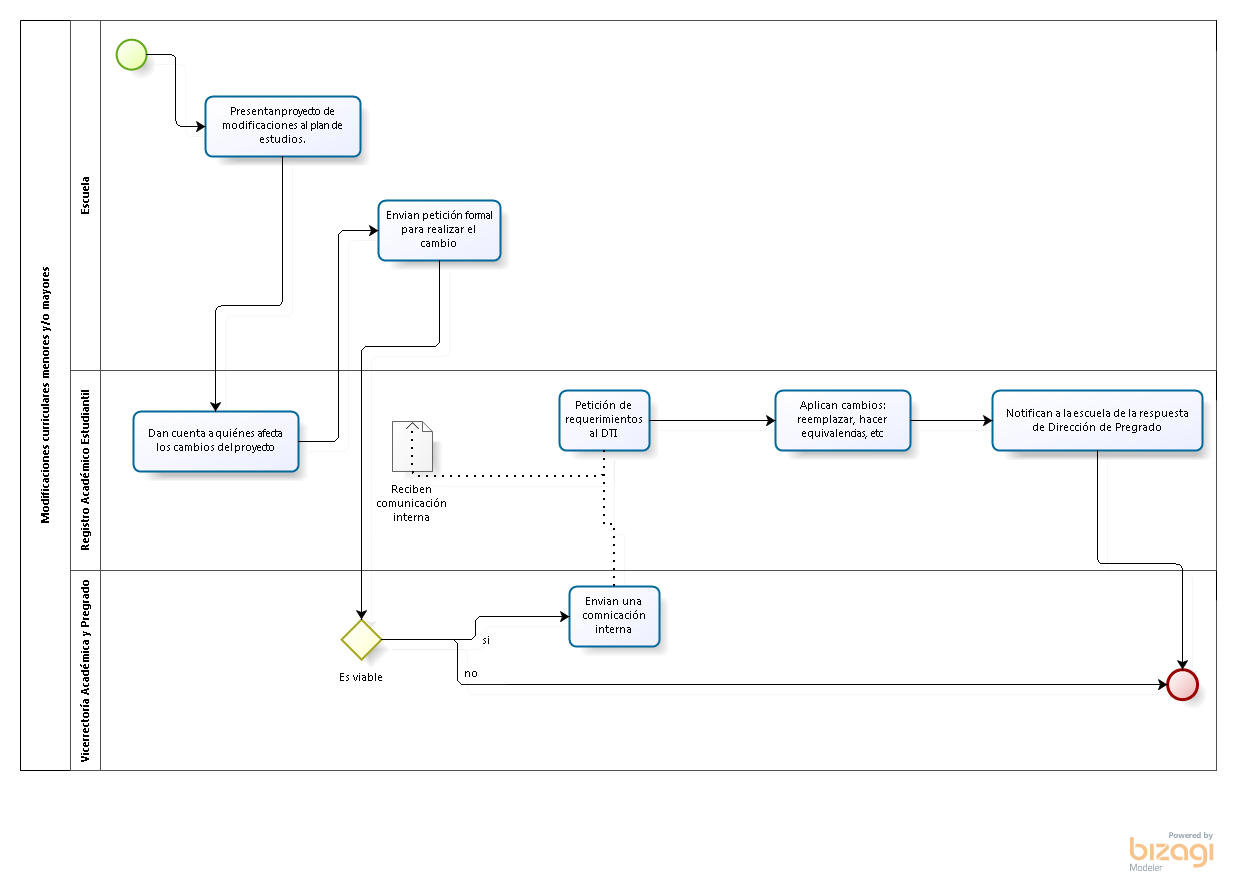
\includegraphics[width=0.9\textwidth]{images/Capitulo_1/Procesos_cambios_curriculares.png}
			\caption[Procesos de cambios Curriculares Mayores y/o menores ]{Procesos de cambios Curriculares Mayores y/o menores  \footnote{}}
			\label{Figura2}
		\end{figure}
		
		\footnotetext{Elaboración propia.}				
		\newpage
		
		
		Dado lo anterior, podemos ver que los procesos curriculares no se gestionan con un sistema informático, no existiendo un software encargado  de almacenar y documentar los cambios que afectan a los proyectos curriculares de las carreras.
		
	



\newpage
%----------------------------------------------------------
%----------------------------------------------------------
\section{MARCO TEÓRICO}
\subsection{Arquitectura MVC?}

\subsection{Tecnologías para el desarrollo de la plataforma}

\subsubsection{Front-end}

Esta capa es la parte del software que interactúa con el o los usuarios, en ésta  se encuentran todas las tecnologías que corren del lado del cliente, es decir, todas aquellas tecnologías que corren del lado del navegador web. Es por ello que es de vital importancia de que el front-end sea capaz de entregar  al usuario todas las herramientas necesarias para que éste pueda realizar una correcta interacción con el sistema. Entre las tecnologías usadas en esta capa se encuentran las habituales en el desarrollo Web, tales como HTML, CSS y JavaScript junto con otras que se describirán a continuación.

\myparagraph{JQuery}

JQuery es una librería JavaScript rápida, liviana y con amplias funcionalidades. Hace mucho más simple tareas como recorrer y manipular un documento HTML, manejar eventos, animaciones, e interacciones Ajax	\footnote{Ajax: Asynchronous JavaScript And XML} por medio de una API fácil de usar que funciona a través de múltiples navegadores. Con una combinación de versatilidad y capacidad de ampliación, esta librería busca cambiar la forma en que las personas escriben JavaScript \cite{JQu15}.
\\

Si bien existen otras librerías de JavaScript (Prototype, MoonTools, entre otros). Se decidió usar JQuery en el proyecto por los siguientes motivos:
\begin{itemize}
	\item Es de uso general, por lo que posee una comunidad activa y una extensa documentación.
	\item Posee una amplia variedad de complementos que facilitan el desarrollo.
	\item Es modular.
	\item Es compatible con todos los navegadores existentes.
\end{itemize}


\myparagraph{Alertify}

Alertify es un script escrito con Jquery, el cual nos permite utilizar los siguientes elementos Javascript personalizados: alert(), confirm() y prompt(). Además también nos permite utilizar sus notificaciones, las cuales son muy agradables y sencillas de utilizar y modificar\cite{ALE15}.
\\

Alertify ha sido construido para personalizar nuestras alertas y notificaciones, de esta manera el front-end de la plataforma es mas amigable al usuario y esto permite un mejor entendimiento de los eventos que se realizan en tiempo de ejecución. Además es un plugin multi-idioma y posee responsive-design \footnote{ \textbf{ Responsive Design} es un nuevo paradigma del desarrollo web. Permite adaptar cada sitio a los diferentes formatos de dispositivos de acceso; smartphones, tabletas, portátiles, etc.}
\\

A pesar de que la mayoría de los plugins de notificaciones presentan inconvenientes al momento de implementar con vb.net, se decidió usar un sistema de alertas principalemente para facilitar la visualización de todos los eventos que ocurren en el sistema.


\myparagraph{Boostrap}

Boostrap fue creado a mediados del 2010 por un diseñador y un desarrollador de la red social Twitter, es un proyecto de código abierto, y es uno de los frameworks de front-end más populares en el mundo. Sirvió como guía de estilo para el desarrollo de herramientas internas en la empresa durante más de un año antes de su lanzamiento público, y continua haciéndolo hoy en día\cite{boo15}.
\\

El uso de un framework hace posible que el desarrollo del front-end sea: Fácil, ya que la mayoría de los framework posee una curva de aprendizaje baja, es decir, poseen una gran eficiencia en el  aprendizaje, lo que permite dominar la mayoría de los componentes en un tiempo reducido; Optimizado para dispositivos móviles, puesto que bootstrap posee todas las reglas CSS necesarias para hacer que los sitios se  adapten dinámicamente a la gran mayoría de pantallas y resoluciones existentes en el mercado.


\myparagraph{Template Metis}

Un template es un conjunto de archivos que determinan la estructura y el aspecto visual de un sitio web, y tiene como ventaja principal disminuir tiempos y costos de desarrollo \cite{gli15}. 
\\

El uso de un template disminuye el tiempo de desarrollo de un diseño web, por lo que el alumno tesista se puede centrar en la funcionalidad del sistema que es lo principal."Metis es una  template de administración gratuito basado en Twitter Bootstrap 3.x"\cite{git15}, fue diseñado por un usuario de gitHub y lo puso a disposición para que cualquier usuario lo pueda utilizar.

\myparagraph{Parsley}



\subsubsection{Back-end}
\subsubsection{capa de datos}


\newpage
%----------------------------------------------------------
%----------------------------------------------------------
\section{SOLUCIÓN PROPUESTA}
En este capítulo, se expone la problemática que aborda este proyecto de tesis. Además, se muestra la solución que se llevará a cabo y luego las herramientas que posibilitarán el desarrollo de lo propuesto anteriormente, con el objetivo de gestionar y reducir los tiempos de espera en diferentes centros de atención altamente concurridos.\\

\subsection{Problemática}

Es recurrente que al momento de realizar un trámite o compras en un centro de atención: bancos, clínicas, sección de carnes en un supermercado, etc., en horas punta exista una probabilidad alta en que el tiempo de espera sea considerable. Este tiempo excesivo, es un hecho generador de desgaste físico y emocional ocasionando daño moral en las personas. Es por ello que las instituciones elaboran estrategias para brindarles una mejor calidad de servicio al optimizar los tiempos de espera. Sin embargo, estos esfuerzos continuan requiriendo más incorporación de tecnología con tal de brindar mayores avances en esta temática.

\subsection{Presentación de la solución}

Para resolver la problemática antes presentada, se propone una solución de gestión de turnos de atención, que contempla su seguimiento en tiempo real. Ésta, consta de tres partes:

\begin{enumerate}
\item Una aplicación móvil que permite obtener los turnos de atención.
\item Almacenamiento de datos.
\item Un módulo web que permite gestionar los turnos de atención y generar reportes utilizando los datos almacenados.
\end{enumerate}

La aplicación móvil, sirve como herramienta para obtener un turno de atención y recibir notificaciones con información del estado de avance de la fila que corresponde al servicio que seleccionó el usuario. Además, ésta envía datos relevantes del dispositivo móvil para ser almacenados en un servidor central.\\

En el párrafo anterior se menciona el almacenamiento de datos en un servidor central. Para hacer efectivo ésto, el servidor cuenta con un sistema de gestión de bases de datos, y una serie de aplicaciones que soportan la comunicación entre la aplicación móvil, dicho servidor y el módulo web.\\

El módulo web mencionado es un sistema que permite gestionar los turnos, coordinar el envío de las notificaciones a los \textit{smartphones} para que los clientes se acerquen al módulo de atención correspondiente y generar reportes que muestran estadísticas sobre los diferentes servicios que brinda el centro de atención en cuestión.\\

\subsection{Descripción de la metodología}

En general el desarrollo del proyecto se basará en la búsqueda en Internet y el continuo apoyo del patrocinante, mostrando avances periódicos e incrementales. El desarrollo del proyecto contempla un marco de trabajo ceñido al ciclo de vida iterativo e incremental, debido a que el contacto con el  profesor patrocinante será constante para validar los avances presentados. Además se realizarán varias pruebas o prototipos iniciales, para comprobar que está correcta la \textbf{comunicación/funcionamiento} entre las diferentes piezas de software que integran el sistema y así evitar posibles complicaciones que signifiquen excesivas horas de dedicación para resolver errores. \\

\textbf{Objetivo Específico 1:} Analizar las principales tecnologías web y sistemas de notificaciones que permitan registrar y realizar el seguimiento de tickets de espera.\\

Se comenzará investigando en Internet lo referente a las tecnologías de notificación disponibles para \textit{Smartphones} y, además se hará una revisión de proyectos similares que estén en funcionamiento. \\

\textbf{Objetivo Específico 2:} Obtener, analizar y especificar los requisitos del sistema, además de analizar y diseñar casos de uso correspondientes con los objetos de diseño necesarios, y generar mockups de la interfaz para el posterior desarrollo del registro vía web y/o aplicación \textit{Android} y seguimiento a través de Notificaciones \textit{Push} de los \textit{tickets} de espera para una oficina de atención de clientes.\\

Primero se deben especificar los requerimientos del sistema a implementar. Se incluirán artefactos UML, interfaz del \textit{software} y un modelo de datos. Además, se debe modelar  la arquitectura que sostendrá este prototipo. Es decir,  el \textit{hardware} y \textit{software} que usará el sistema.\\

\textbf{Objetivo Específico 3:} Implementar el prototipo funcional de acuerdo a lo modelado en los objetivos específicos anteriores.\\

Se deberá implementar el prototipo en base a todas las normas y especificaciones descritas anteriormente, con la construcción de una interfaz de usuario amigable, soportado por una base de datos disponible en el servidor del sistema.\\

\textbf{Objetivo Específico 4:} Diseñar e implementar un Sistema web de reportes, que permita gestionar los datos obtenidos en este proceso.\\

Primero se debe contar con la especificacion de requerimientos para este sistema web de reportes e incluir artefactos UML. Después se desarrollará el sistema Web de reportes, a partir de la información obtenida y almacenada del proceso de: inscripción, notificación y atención. Esto permitirá gestionar los procesos de atención.\\


\subsection{Descripción de Tecnologías a utilizar}

En esta sección, se retomará el tema tratado en el punto 2.1, con la diferencia que aquí se justificará el por qué de la elección de la tecnología escogida entre todas las disponibles.\\

\subsubsection{Entorno de desarrollo}

Un entorno de desarrollo integrado (IDE) permite a un programador escribir código fuente, compilar, interpretar o ambos en algunos casos. Para escribir la aplicación móvil de este proyecto, se utilizó el IDE Android Studio 1.0\footnote{http://developer.android.com/tools/studio/index.html}. Básicamente fué elegido sobre el tradicional Eclipse pues todo apunta a que será el entorno de desarrollo recomendado por el equipo de \textit{Android}.\\

\subsubsection{Intercambio de datos}

Se usará el modelo cliente-servidor para el intercambio de datos entre la aplicación móvil, el servidor central y el almacenamiento de información desde el módulo web. Para hacer efectiva esta comunicación, se utilizará el servidor web HTTP Apache, que se encargará de recibir y responder las peticiones de: la aplicación móvil y módulo web.

Para manipular las peticiones, se usará un servicio web escrito en el lenguaje de programación PHP, que se ocupará de distinguir las solicitudes que llegarán y responder pertinentemente a ellas. Como por ejemplo, almacenar información de un dispositivo nuevo, u obtener la última notificación recibida.\\

La aplicación móvil necesita de un medio para comunicarse con el servicio web alojado en el servidor central. Para ello, ese medio corresponde a un formato ligero de intercambio de datos que sea sencillo de leer y escribir para humanos. Por lo tanto, se optó por utilzar la Notación de Objetos JavaScript JSON, debido a su simplicidad en relación a XML. JSON básicamente describe los datos con una sintaxis dedicada que se usa para identificar y gestionar los datos.\\

JSON consta de dos estructuras:

\begin{enumerate}
\item Una colección de pares nombre/valor. En la mayoría de los lenguajes se conoce como un objeto, registro o \textit{struct\footnote{http://c.conclase.net/curso/?cap=011}}, tabla \textit{hash}.
\item Una lista ordenada de valores. Esto en la mayoría de los lenguajes se conoce como arreglos, listas.
\end{enumerate}

A modo explicativo y con el propósito de aclarar la estructura de JSON, en las figuras a siguientes se entrega un detalle de los dos puntos antes descritos.\\

Un Objeto es un conjunto desordenado de pares nombre/valor. Comienza con \{(llave de apertura) y termina con \} (llave de cierre). El nombre es seguido por : (dos puntos) y los pares nombre/valor están separados por , (coma). Lo anterior, se aprecia en la máquina de estado finito en la Figura 5.\\

\begin{figure}[H]
\centering
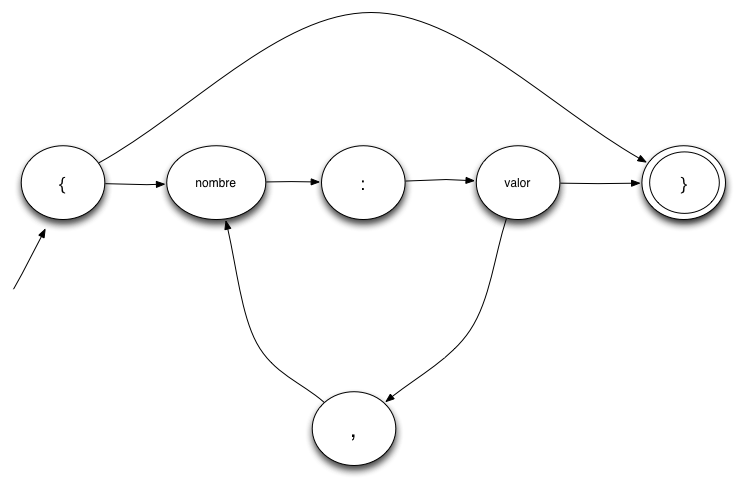
\includegraphics[scale=0.50]{images/capitulo3/afd1.png}
\caption{\textbf{Objeto:} conjunto desordenado de pares nombre/valor.}
\label{objeto}
\end{figure}

Un arreglo es una colección de valores, que comienza con [(corchete izquierdo) y termina con ] (corchete derecho). Los valores son separados por , (coma). Lo anterior, se aprecia en la máquina de estado finito en la Figura 6.\\

\begin{figure}[H]
\centering
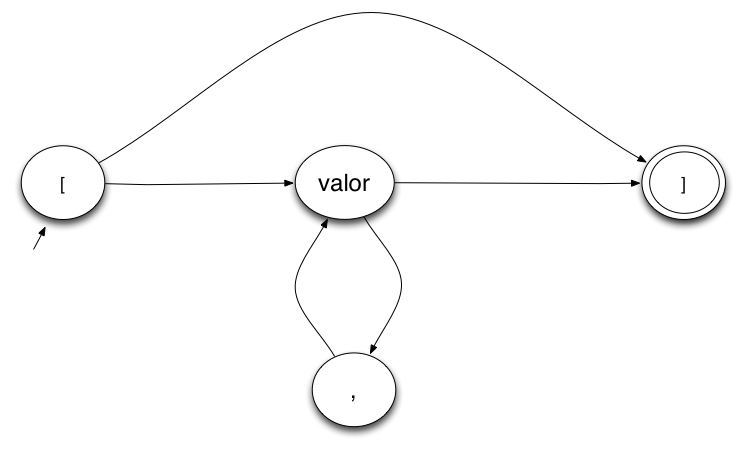
\includegraphics[scale=0.50]{images/capitulo3/afd2.png}
\caption{\textbf{Arreglo:} colección de valores separados por ',' (coma).}
\label{arreglo}
\end{figure}

Un valor puede ser una cadena de caracteres, o número, u objeto, o arreglo, o true, o false, o null.  Lo anterior, se aprecia en la máquina de estado finito en la Figura 7.\\

\begin{figure}[H]
\centering
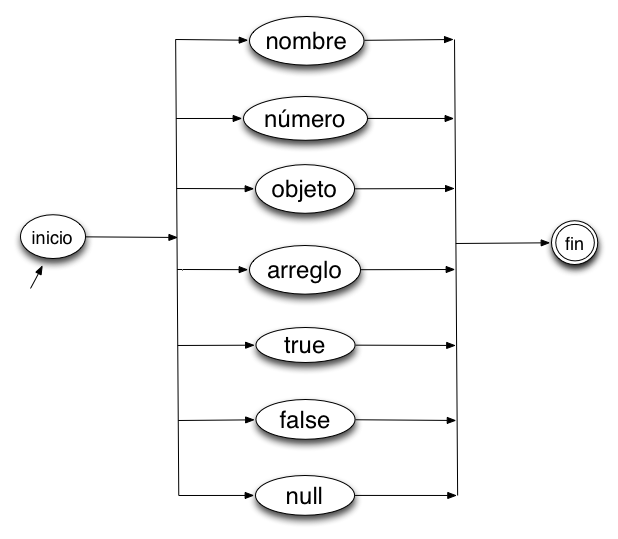
\includegraphics[scale=0.50]{images/capitulo3/afd3.png}
\caption{\textbf{Valor:} cadena de caracteres, o número, u objeto, o arreglo, o true, o false, o null.}
\label{valor}
\end{figure}

\subsubsection{Base de datos}

Para almacenar los datos proporcionados por la aplicación móvil y el módulo web,  se utilizará el sistema de gestión de bases de datos relacionales MySQL. En este apartado no se ahondará  sobre este sistema pues fue descrito en el capítulo anterior, en el punto 2.1.5.\\

\subsubsection{Librerías utilizadas}

La única librería incluída en el proyecto y que hace posible la comunicación entre la aplicación móvil y GCM: enviar y recibir notificaciones es la librería de GoogleCloudMessaging. Ésta debe ser incluida en el proyecto en \textit{Android Studio} para utilizar sus clases desde nuestra aplicación.\\

\subsubsection{Patrón MVC}

El acrónimo MVC corresponde a: \textbf{Modelo} - \textbf{Vista} - \textbf{Controlador}. Éste es un patrón de arquitectura de \textit{software} donde en una aplicación separa los datos y la lógica del negocio de la interfaz de usuario y el módulo que se encarga de gestionar los eventos y comunicaciones. Por lo anterior, MVC propone que se construyan tres componentes diferentes: el modelo, la vista y el controlador y que al final se relacionarán para tener como resultado una aplicación, en el caso del proyecto una aplicación móvil.\\ 

Para entender la Figura 8, se explicará brevemente de qué se trata cada uno de los componentes de este modelo.\\

\begin{figure}[H]
\centering
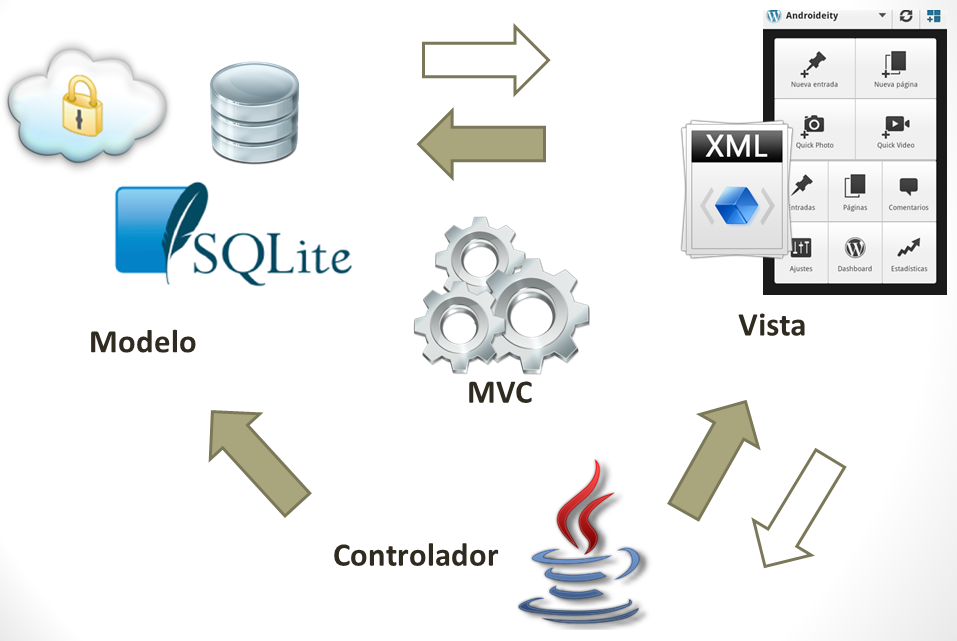
\includegraphics[scale=0.50]{images/capitulo3/mvc.png}
\caption{Patrón MVC.\cite{And12}}
\label{valor}
\end{figure}

\begin{enumerate}
\item \textbf{Modelo:} Básicamente el modelo corresponde a qué base de datos o servicios web se utilizará para almacenar la información. El modelo a elegir depende directamente de las necesidades de información que tenga la aplicación que se desarrollará.
\item \textbf{Vista:} La vista no es mas que la interfaz con la que va a interactuar el usuario. En \textit{Android}, las interfaces se construyen en XML, y es a través de éstas que se presentan los datos a los usuarios.
\item \textbf{Controlador:} Son las clases que contienen el código y permiten darle vida a las interfaces construidas permitiendo desplegar y consumir información de/para el usuario. En un proyecto \textit{Android} los controladores corresponden a las clases programadas en lenguaje JAVA y son el núcleo de la aplicación.
\end{enumerate}

\subsection{Arquitectura del sistema}

En los puntos anteriores se ha descrito lo concerniente a cómo y qué tecnologías se utilizarán para dar solución al problema expuesto. Por último, para dar sentido a lo antes planteado en los tópicos anteriores, es factible definir una arquitectura para el sistema. Ver Figura 9. La arquitectura planteada, se compone de un servidor central provisto de diversos servicios, \textit{smartphones} que se comunicarán con el sistema, una base de datos para almacenar la información, un monitor que mostrará el turno que está siendo atendido, el servicio de GCM por el cual circulan las notificaciones y un módulo web de reportes. 

\begin{figure}[H]
\centering
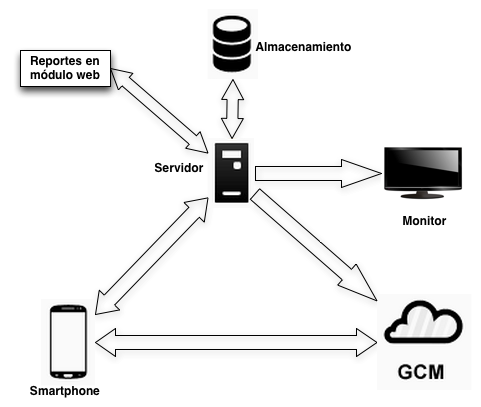
\includegraphics[scale=0.70]{images/capitulo3/arquitectura.png}
\caption{Arquitectura del sistema.}
\label{arquitectura}
\end{figure}

\newpage
%----------------------------------------------------------
%----------------------------------------------------------
\section{ANÁLISIS Y DISEÑO DEL PROTOTIPO DEL SISTEMA}
En este capítulo se explican y detallan las etapas que permiten modelar la solución propuesta utilizando artefactos de \textit{software}, que permiten documentar el sistema bajo el marco de trabajo de una metodología de desarrollo de \textit{software}.


\subsection{Metodología}

Una metodología de desarrollo de \textit{software} puede ser definida como un marco de trabajo que se utiliza para estructurar, planificar y controlar el proceso correspondiente al desarrollo de un sistema de información. Para una administración y gestión sistemática de todo proyecto de \textit{software}, y llevarlo a cabo con altas posibilidades de éxito, es necesario guiarse por una metodología, permitiendo así dividir un proyecto en módulos o etapas. De esta forma estructurada y organizada es posible crear, desarrollar y mantener un sistema desde que surge la necesidad del producto hasta que se cumple el objetivo por el cual fue desarrollado.\\

En este proyecto se utilizará el ciclo de vida incremental para el desarrollo del \textit{software}, ya que este modelo se acomoda bastante a la implementación de un prototipo, que es el caso de este proyecto de tesis. Además, no es necesario disponer de los requerimientos de todas las funcionalidades en el comienzo del mismo. El proceso consiste en ir construyendo módulos o iteraciones que van cumpliendo con las diferentes funciones del sistema, aumentando gradualmente las capacidades de éste. Las ventajas de este ciclo de vida son:

\begin{enumerate}
\item Desarrollar las funcionalidades por etapas permite detectar si los requerimientos planteados para los niveles siguientes son correctos.
\item En caso de enfrentarse ante un error grave solo se desecha la última iteración.
\item Construir por etapas, partes pequeñas del sistema, representa menos riesgo que construir un sistema grande.
\end{enumerate}


\subsection{Plan de trabajo}

En la Figura 10 se ilustra el plan de trabajo para llevar a cabo la implementación del sistema:

\begin{figure}[H]
\centering
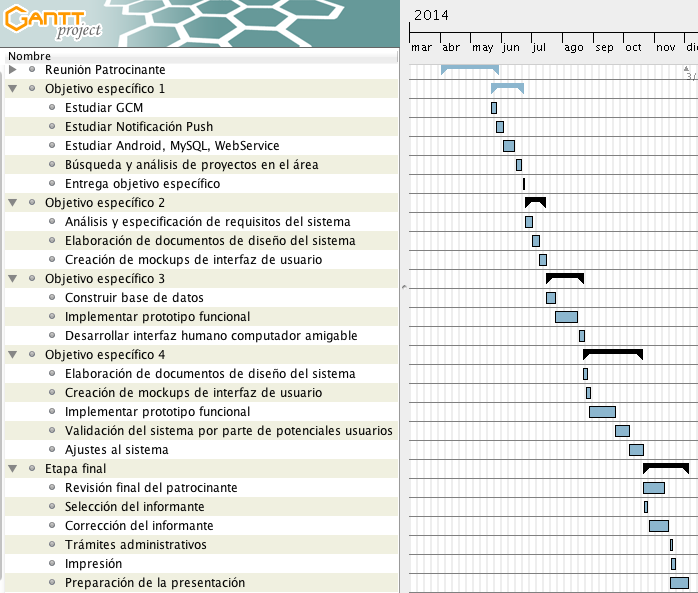
\includegraphics[scale=0.65]{images/capitulo4/gantt.png}
\caption{Carta Gantt que exhibe las etapas de desarrollo del sistema.}
\label{gantt}
\end{figure}


\subsubsection{Estrategia de implementación}

A través del proceso de implementación y desarrollo del software, se tuvo que tomar en cuenta lo siguiente:

\begin{enumerate}
\item Es importante reunirse con el profesor patrocinante al comienzo, durante y al término de una iteración, para así aclarar y resolver requerimientos específicos del sistema que puedan surgir.
\item Durante el desarrollo del sistema, se consideran presentaciones de avance de las iteraciones de tal forma que se disminuyan errores y/o riesgos en la entrega final.
\item El producto final se dará terminado cuando se hayan cumplido todos los requisitos del sistema.
\end{enumerate}

\subsection{Análisis}

\subsubsection{Descripción de los actores del sistema}

\textbf{Administrador:} es un individuo que se ocupa de configurar el sistema, antes de la puesta en marcha, y tiene acceso a todas las funcionalidades del mismo. Es decir, es un funcionario del centro de atención donde sea instalado el sistema de gestión de tickets.\\

\textbf{Ejecutivo:} es un funcionario del centro de atención que utilza el sistema para realizar las llamadas a los clientes cuando sea oportuno. Tiene acceso limitado a la aplicación web.\\

\textbf{Cliente:} corresponde a una persona que interactúa como cliente con el sistema a través de la aplicación móvil desde su \textit{smartphone} en un centro de atención. \\

\subsubsection{Casos de Uso}

\begin{figure}[H]
\centering
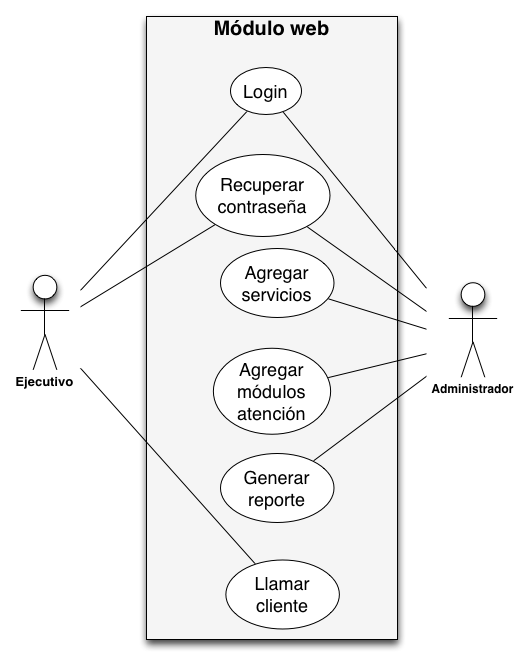
\includegraphics[scale=0.65]{images/capitulo4/moduloWeb.png}
\caption{Diagrama de Casos de Uso Módulo web.}
\label{cuModuloWeb}
\end{figure}

\begin{figure}[H]
\centering
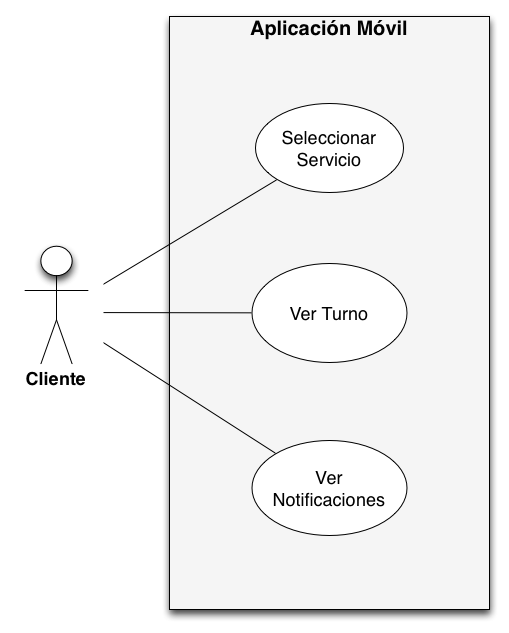
\includegraphics[scale=0.60]{images/capitulo4/appMovil.png}
\caption{Diagrama de Casos de Uso Aplicación Móvil.}
\label{cuAppMovil}
\end{figure}

\subsection{Especificación de requerimientos}

De acuerdo a la problemática y objetivos descritos se tomaron y obtuvieron los requisitos para poder desarrollar el Sistema de Gestión de tickes de espera.

\subsubsection{Requisitos Funcionales}

Cuando se plantea una solución a una problemática, nacen ideas de cómo será y qué características tendrá el sistema que se desarrollará. Éstas características requeridas del \textit{software} tienen relación con una capacidad de acción que tendrá el nuevo sistema, es decir, una funcionalidad.\\ 

A continuación en la tabla 3 se presentan los requisitos funcionales extraídos de los diagramas UML y de las capacidades que se desea que tenga el sistema a implementar.

\begin{spacing}{1.0}
\begin{table}[H]
\centering
\caption{Requisitos Funcionales.} 
\begin{tabular}{|c|c|}
\hline 
\rowcolor{gray!30} &\\
\rowcolor{gray!30} \textbf{Ref. \#} & \textbf{Función} \\ 
\rowcolor{gray!30} &\\
\hline 
&\\[-0.2cm]
FRQ-001 & Iniciar sesión en aplicación web.\\
\hline
&\\[-0.2cm]
FRQ-002 & Cargar y mostrar servicios.\\
\hline
&\\[-0.2cm]
FRQ-003 & Cargar y mostrar módulos de atención.\\
\hline
&\\[-0.2cm]
FRQ-004 & Enviar notificaciones desde aplicación web a \textit{smartphone}.\\ 
\hline
&\\[-0.2cm]
FRQ-005 & Generar reportes.\\
\hline
&\\[-0.2cm]
FRQ-006 & Mostrar últimos turnos en atención.\\
\hline
&\\[-0.2cm]
FRQ-007 & Monitor de atenciones.\\
\hline
&\\[-0.2cm]
FRQ-008 & Mostrar servicios.\\
\hline
&\\[-0.2cm]
FRQ-009 & Selecionar un servicio.\\ 
\hline
&\\[-0.2cm]
FRQ-010 & Ver turno de atención.\\
\hline
&\\[-0.2cm]
FRQ-011 & Ver notificaciones.\\
\hline
&\\[-0.2cm]
FRQ-012 & Mostrar notificaciones nuevas automáticamente.\\
\hline
&\\[-0.2cm]
FRQ-013 & Mostrar información de la aplicación.\\
\hline
\end{tabular}
\label{tabla_pila}
\end{table}
\end{spacing}

\subsubsection{Requisitos No Funcionales}

Los requisitos no funcionales, obedecen a todas las exigencias cualitativas que se imponen, es decir, cómo debe ser el sistema. Generalmente corresponden a requisitos que son restricciones que se deben cumplir y que se encuentran fuera del conjunto de los requisitos funcionales. A continuación en la tabla 4 se especifican los requisitos no funcionales del sistema.

\begin{spacing}{1.0}
\begin{table}[H]
\centering
\caption{Requisitos No Funcionales.} 
\begin{tabular}{|c|c|}
\hline 
\rowcolor{gray!30} &\\
\rowcolor{gray!30} \textbf{Ref. \#} & \textbf{Función} \\ 
\rowcolor{gray!30} &\\
\hline 
&\\[-0.2cm]
FRQ-014 & Interfaz del sistema debe ser amigable con el usuario.\\
\hline
&\\[-0.2cm]
FRQ-015 & Bajo tráfico de datos.\\
\hline
&\\[-0.2cm]
FRQ-016 & Portabilidad.\\
\hline
&\\[-0.2cm]
FRQ-017 & La aplicación móvil debe ser desarrollada para Android.\\
\hline
\end{tabular}
\label{tabla_pila}
\end{table}
\end{spacing}



\myparagraph{Casos de Uso Extendido del sistema}


\begin{spacing}{1.0}
	\begin{table}[H]
		\centering
		\caption{Caso de uso extendido ``Agregar Servicios''.} 
		\begin{tabular}{| >{\arraybackslash\columncolor{gray!30}}p{3.1cm}| >{\arraybackslash}p{10.4cm}|}
			\hline 
			\rowcolor{gray!30} &\\[-0.2cm]
			\rowcolor{gray!30} \textbf{Caso de uso:} & \textbf{Agregar Servicios (CU01).} \\[0.2cm]
			\hline
			&\\[-0.2cm]
			\textbf{Actores:} & Administrador. \\[0.2cm]
			\hline
			&\\[-0.2cm]
			\textbf{Propósito:} & Agregar servicios al sistema. \\[0.2cm]
			\hline
			&\\[-0.2cm]
			\textbf{Resumen:} & El Administrador agrega todos los servicios que brinda el centro de atención, a la base de datos ubicada en el servidor central. \\[0.2cm]
			\hline
			&\\[-0.2cm]
			\textbf{Tipo:} & Primario y esencial. \\[0.2cm]
			\hline
			&\\[-0.2cm]
			\textbf{Precondiciones:} & {\tiny$\blacksquare$} La base de datos, servidor web y servidor central deben estar operativos. \\[0.2cm]
			\hline
			\multicolumn{2}{| >{\arraybackslash\columncolor{gray!30}}c|}{}\\[-0.2cm]
			\multicolumn{2}{| >{\arraybackslash\columncolor{gray!30}}c|}{\textbf{Curso normal de los eventos}}\\[0.2cm]
		\end{tabular}
		
		\vspace{-0.5cm}
		\begin{center}
			\begin{tabular}{| >{\arraybackslash}p{6.75cm} | >{\arraybackslash}p{6.75cm} |}
				\hline
				\rowcolor{gray!30} &\\[-0.2cm]
				\rowcolor{gray!30} \textbf{Acción de los actores} & \textbf{Respuesta del sistema}\\[0.2cm]
				\hline
				&\\[-0.2cm]
				\textbf{1.} Este caso de uso comienza cuando se debe preparar el sistema para ser utilizado en el centro de atención. & \\
				\textbf{2.} El Administrador se dirige a la opción que le permite agregar un servicio. &\\
				& \textbf{3.} Muestra la interfaz para realizar esta acción. \\
				\textbf{4.} El Administrador ingresa el nombre del servicio y agrega el servicio al sistema. & \\
				& \textbf{5.} La base de datos recibe y graba la información. \\
				& \textbf{6.} El servicio es agregado y se muestra en la ventana. \\
				\hline
				\multicolumn{2}{| >{\arraybackslash\columncolor{gray!30}}c|}{}\\[-0.2cm]
				\multicolumn{2}{| >{\arraybackslash\columncolor{gray!30}}c|}{\textbf{Cursos alternativos}}\\[0.2cm]
				\hline
				\multicolumn{2}{|l|}{}\\[-0.2cm]
				\multicolumn{2}{|l|}{\textbf{4.} El servicio ya existe.}\\
				\multicolumn{2}{|l|}{\textbf{5.} El sistema no responde ante el envío de los datos.}\\
			\end{tabular}
		\end{center}
		
		\vspace{-0.5cm}
		\begin{tabular}{| >{\arraybackslash\columncolor{gray!30}}p{3.1cm}| >{\arraybackslash}p{10.4cm}|}
			\hline
			&\\[-0.2cm]
			\textbf{Post condiciones:} & El sistema queda esperando para repetir el proceso o realizar uno diferente. \\[0.2cm]
			\hline
		\end{tabular}
		
		\label{tabla_CU01}
	\end{table}
\end{spacing}


\begin{spacing}{1.0}
	\begin{table}[H]
		\centering
		\caption{Caso de uso extendido ``Agregar Módulo Atención''.} 
		\begin{tabular}{| >{\arraybackslash\columncolor{gray!30}}p{3.1cm}| >{\arraybackslash}p{10.4cm}|}
			\hline 
			\rowcolor{gray!30} &\\[-0.2cm]
			\rowcolor{gray!30} \textbf{Caso de uso:} & \textbf{Agregar Módulo Atención (CU02).} \\[0.2cm]
			\hline
			&\\[-0.2cm]
			\textbf{Actores:} & Administrador. \\[0.2cm]
			\hline
			&\\[-0.2cm]
			\textbf{Propósito:} & Agregar módulos de atencion al sistema. \\[0.2cm]
			\hline
			&\\[-0.2cm]
			\textbf{Resumen:} & El Administrador agrega tal sistema todos los módulos donde se atenderán clientes. \\[0.2cm]
			\hline
			&\\[-0.2cm]
			\textbf{Tipo:} & Primario y esencial. \\[0.2cm]
			\hline
			&\\[-0.2cm]
			\textbf{Precondiciones:} & {\tiny$\blacksquare$} La base de datos, servidor web y servidor central deben estar operativos. \\[0.2cm]
			\hline
			\multicolumn{2}{| >{\arraybackslash\columncolor{gray!30}}c|}{}\\[-0.2cm]
			\multicolumn{2}{| >{\arraybackslash\columncolor{gray!30}}c|}{\textbf{Curso normal de los eventos}}\\[0.2cm]
		\end{tabular}
		
		\vspace{-0.5cm}
		\begin{center}
			\begin{tabular}{| >{\arraybackslash}p{6.75cm} | >{\arraybackslash}p{6.75cm} |}
				\hline
				\rowcolor{gray!30} &\\[-0.2cm]
				\rowcolor{gray!30} \textbf{Acción de los actores} & \textbf{Respuesta del sistema}\\[0.2cm]
				\hline
				&\\[-0.2cm]
				\textbf{1.} Este caso de uso comienza luego de que el Administrador haya ingresado los servicios (CU01). & \\
				\textbf{2.} El Administrador se dirige a la opción que le permite agregar un módulo de atención. &\\
				& \textbf{3.} Muestra la interfaz para realizar esta acción. \\
				\textbf{4.} El Administrador ingresa el nombre del módulo de atención y lo agrega al sistema. & \\
				& \textbf{5.} La base de datos recibe y graba la información. \\
				& \textbf{6.} El módulo de atención es agregado y se muestra en la ventana. \\
				\hline
				\multicolumn{2}{| >{\arraybackslash\columncolor{gray!30}}c|}{}\\[-0.2cm]
				\multicolumn{2}{| >{\arraybackslash\columncolor{gray!30}}c|}{\textbf{Cursos alternativos}}\\[0.2cm]
				\hline
				\multicolumn{2}{|l|}{}\\[-0.2cm]
				\multicolumn{2}{|l|}{\textbf{4.} El módulo de atención ya existe.}\\
				\multicolumn{2}{|l|}{\textbf{5.} El sistema no responde ante el envío de los datos.}\\
			\end{tabular}
		\end{center}
		
		\vspace{-0.5cm}
		\begin{tabular}{| >{\arraybackslash\columncolor{gray!30}}p{3.1cm}| >{\arraybackslash}p{10.4cm}|}
			\hline
			&\\[-0.2cm]
			\textbf{Post condiciones:} & El sistema queda esperando para repetir el proceso o realizar uno diferente. \\[0.2cm]
			\hline
		\end{tabular}
		
		\label{tabla_CU02}
	\end{table}
\end{spacing}

\begin{spacing}{1.0}
	\begin{table}[H]
		\centering
		\caption{Caso de uso extendido ``Seleccionar Servicio''.} 
		\begin{tabular}{| >{\arraybackslash\columncolor{gray!30}}p{3.1cm}| >{\arraybackslash}p{10.4cm}|}
			\hline 
			\rowcolor{gray!30} &\\[-0.2cm]
			\rowcolor{gray!30} \textbf{Caso de uso:} & \textbf{Seleccionar Servicio (CU03).} \\[0.2cm]
			\hline
			&\\[-0.2cm]
			\textbf{Actores:} & Cliente. \\[0.2cm]
			\hline
			&\\[-0.2cm]
			\textbf{Propósito:} & Obtener un turno de atención. \\[0.2cm]
			\hline
			&\\[-0.2cm]
			\textbf{Resumen:} & El usuario se abre la aplicación \textbf{Mi Turno} y presiona un servicio, mostrado en la pantalla principal, para obtener un turno de atención. \\[0.2cm]
			\hline
			&\\[-0.2cm]
			\textbf{Tipo:} & Primario y esencial. \\[0.2cm]
			\hline
			&\\[-0.2cm]
			\textbf{Precondiciones:} & {\tiny$\blacksquare$} El dispositivo móvil debe tener conexión a Internet. \\
			& {\tiny$\blacksquare$} La base de datos, servidor web y servidor central deben estar operativos. \\ [0.2cm]
			\hline
			\multicolumn{2}{| >{\arraybackslash\columncolor{gray!30}}c|}{}\\[-0.2cm]
			\multicolumn{2}{| >{\arraybackslash\columncolor{gray!30}}c|}{\textbf{Curso normal de los eventos}}\\[0.2cm]
		\end{tabular}
		
		\vspace{-0.5cm}
		\begin{center}
			\begin{tabular}{| >{\arraybackslash}p{6.75cm} | >{\arraybackslash}p{6.75cm} |}
				\hline
				\rowcolor{gray!30} &\\[-0.2cm]
				\rowcolor{gray!30} \textbf{Acción de los actores} & \textbf{Respuesta del sistema}\\[0.2cm]
				\hline
				&\\[-0.2cm]
				\textbf{1.} Este caso de uso comienza cuando un Cliente se acerca a un centro de atención y, desea obtener un turno para realizar un trámite en algún servicio del centro de atención. & \\
				\textbf{2.} El Cliente presiona un botón correspondiente al servicio que desea. &\\
				& \textbf{3.} Muestra un cuadro de diálogo donde pregunta \textbf{¿Desea obtener ticket de atención?}. \\
				& \textbf{5.} Muestra un mensaje confirmando la acción. \\
				&\textbf{6.} Muestra una nueva pantalla donde se indica el \textbf{Turno} y \textbf{Servicio}. \\
				\hline
				\multicolumn{2}{| >{\arraybackslash\columncolor{gray!30}}c|}{}\\[-0.2cm]
				\multicolumn{2}{| >{\arraybackslash\columncolor{gray!30}}c|}{\textbf{Cursos alternativos}}\\[0.2cm]
				\hline
				\multicolumn{2}{|l|}{}\\[-0.2cm]
				\multicolumn{2}{|l|}{\textbf{4.} El Cliente presionó equivocadamente el servicio y presiona el botón \textbf{NO}.}\\
				\multicolumn{2}{|l|}{\textbf{5.} El dispositivo móvil pierde comunicación con el servidor central.}\\
			\end{tabular}
		\end{center}
		
		\vspace{-0.5cm}
		\begin{tabular}{| >{\arraybackslash\columncolor{gray!30}}p{3.1cm}| >{\arraybackslash}p{10.4cm}|}
			\hline
			&\\[-0.2cm]
			\textbf{Post condiciones:} & La aplicación móvil queda trabajando en segundo plano a la espera de recibir Notificaciones. \\[0.2cm]
			\hline
		\end{tabular}
		
		\label{tabla_CU03}
	\end{table}
\end{spacing}

\subsection{Diseño}

\subsubsection{Casos de Uso Real}

\begin{spacing}{1.0}
	\begin{table}[H]
		\centering
		\caption{Caso de uso Real ``Agregar Servicios''.} 
		\begin{tabular}{| >{\arraybackslash\columncolor{gray!30}}p{3.1cm}| >{\arraybackslash}p{10.4cm}|}
			\hline 
			\rowcolor{gray!30} &\\[-0.2cm]
			\rowcolor{gray!30} \textbf{Caso de uso:} & \textbf{Agregar Servicios (CU01).} \\[0.2cm]
			\hline
			&\\[-0.2cm]
			\textbf{Actores:} & Administrador. \\[0.2cm]
			\hline
			&\\[-0.2cm]
			\textbf{Propósito:} & Agregar servicios al sistema. \\[0.2cm]
			\hline
			&\\[-0.2cm]
			\textbf{Resumen:} & El Administrador agrega todos los servicios que brinda el centro de atención, a la base de datos ubicada en el servidor central. \\[0.2cm]
			\hline
			&\\[-0.2cm]
			\textbf{Tipo:} & Primario y esencial. \\[0.2cm]
			\hline
			&\\[-0.2cm]
			\textbf{Precondiciones:} & {\tiny$\blacksquare$} La base de datos, servidor web y servidor central deben estar operativos. \\[0.2cm]
			\hline
			\multicolumn{2}{| >{\arraybackslash\columncolor{gray!30}}c|}{}\\[-0.2cm]
			\multicolumn{2}{| >{\arraybackslash\columncolor{gray!30}}c|}{\textbf{Curso normal de los eventos}}\\[0.2cm]
		\end{tabular}
		
		\vspace{-0.5cm}
		\begin{center}
			\begin{tabular}{| >{\arraybackslash}p{6.75cm} | >{\arraybackslash}p{6.75cm} |}
				\hline
				\rowcolor{gray!30} &\\[-0.2cm]
				\rowcolor{gray!30} \textbf{Acción de los actores} & \textbf{Respuesta del sistema}\\[0.2cm]
				\hline
				&\\[-0.2cm]
				\textbf{1.} Este caso de uso comienza cuando se debe preparar el sistema para ser utilizado en el centro de atención. & \\
				\textbf{2.} El Administrador se dirige a la opción \textbf{Configuración} \textbf{(A)}, luego a \textbf{Agregar Servicios} \textbf{(B)}. &\\
				& \textbf{3.} Muestra la interfaz para realizar esta acción. \\
				\textbf{4.} El Administrador ingresa el nombre del servicio en la entrada de texto \textbf{(C)} y presiona el boton \textbf{Agregar} \textbf{(D)}. & \\
				& \textbf{5.} La base de datos recibe y graba la información. \\
				& \textbf{6.} El servicio es agregado y se muestra en la lista de servicios \textbf{(E)}. \\
				\hline
				\multicolumn{2}{| >{\arraybackslash\columncolor{gray!30}}c|}{}\\[-0.2cm]
				\multicolumn{2}{| >{\arraybackslash\columncolor{gray!30}}c|}{\textbf{Cursos alternativos}}\\[0.2cm]
				\hline
				\multicolumn{2}{|l|}{}\\[-0.2cm]
				\multicolumn{2}{|l|}{\textbf{4.} El servicio ya existe.}\\
				\multicolumn{2}{|l|}{\textbf{5.} El sistema no responde ante el envío de los datos.}\\
			\end{tabular}
		\end{center}
		
		\vspace{-0.5cm}
		\begin{tabular}{| >{\arraybackslash\columncolor{gray!30}}p{3.1cm}| >{\arraybackslash}p{10.4cm}|}
			\hline
			&\\[-0.2cm]
			\textbf{Post condiciones:} & El sistema queda esperando para repetir el proceso o realizar uno diferente. \\[0.2cm]
			\hline
		\end{tabular}
		
		\label{tabla_CU01}
	\end{table}
\end{spacing}

\begin{figure}[H]
\centering
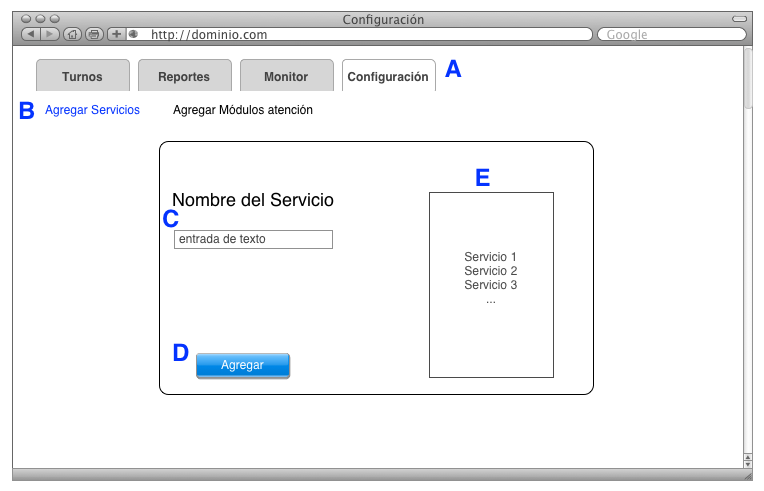
\includegraphics[scale=0.55]{images/capitulo4/mockupCU01.png}
\caption{\textit{Mockup} Caso de Uso 1 (CU01).}
\label{mockupCU01}
\end{figure}


\begin{spacing}{1.0}
	\begin{table}[H]
		\centering
		\caption{Caso de uso Real ``Agregar Módulo Atención''.} 
		\begin{tabular}{| >{\arraybackslash\columncolor{gray!30}}p{3.1cm}| >{\arraybackslash}p{10.4cm}|}
			\hline 
			\rowcolor{gray!30} &\\[-0.2cm]
			\rowcolor{gray!30} \textbf{Caso de uso:} & \textbf{Agregar Módulo Atención (CU02).} \\[0.2cm]
			\hline
			&\\[-0.2cm]
			\textbf{Actores:} & Administrador. \\[0.2cm]
			\hline
			&\\[-0.2cm]
			\textbf{Propósito:} & Agregar módulos de atencion al sistema. \\[0.2cm]
			\hline
			&\\[-0.2cm]
			\textbf{Resumen:} & El Administrador agrega tal sistema todos los módulos donde se atenderán clientes. \\[0.2cm]
			\hline
			&\\[-0.2cm]
			\textbf{Tipo:} & Primario y esencial. \\[0.2cm]
			\hline
			&\\[-0.2cm]
			\textbf{Precondiciones:} & {\tiny$\blacksquare$} La base de datos, servidor web y servidor central deben estar operativos. \\[0.2cm]
			\hline
			\multicolumn{2}{| >{\arraybackslash\columncolor{gray!30}}c|}{}\\[-0.2cm]
			\multicolumn{2}{| >{\arraybackslash\columncolor{gray!30}}c|}{\textbf{Curso normal de los eventos}}\\[0.2cm]
		\end{tabular}
		
		\vspace{-0.5cm}
		\begin{center}
			\begin{tabular}{| >{\arraybackslash}p{6.75cm} | >{\arraybackslash}p{6.75cm} |}
				\hline
				\rowcolor{gray!30} &\\[-0.2cm]
				\rowcolor{gray!30} \textbf{Acción de los actores} & \textbf{Respuesta del sistema}\\[0.2cm]
				\hline
				&\\[-0.2cm]
				\textbf{1.} Este caso de uso comienza luego de que el Administrador haya ingresado los servicios (CU01). & \\
				\textbf{2.} El Administrador se dirige a la opción \textbf{Configuración} \textbf{(A)}, luego a \textbf{Agregar Servicios} \textbf{(B)}. &\\
				& \textbf{3.} Muestra la interfaz para realizar esta acción. \\
				\textbf{4.} El Administrador ingresa el nombre del módulo de atención en la entrada de texto \textbf{(C)} y presiona el boton \textbf{Agregar} \textbf{(D)}. & \\
				& \textbf{5.} La base de datos recibe y graba la información. \\
				& \textbf{6.} El módulo de atención es agregado y se muestra en la lista de servicios \textbf{(E)} \\
				\hline
				\multicolumn{2}{| >{\arraybackslash\columncolor{gray!30}}c|}{}\\[-0.2cm]
				\multicolumn{2}{| >{\arraybackslash\columncolor{gray!30}}c|}{\textbf{Cursos alternativos}}\\[0.2cm]
				\hline
				\multicolumn{2}{|l|}{}\\[-0.2cm]
				\multicolumn{2}{|l|}{\textbf{4.} El módulo de atención ya existe.}\\
				\multicolumn{2}{|l|}{\textbf{5.} El sistema no responde ante el envío de los datos.}\\
			\end{tabular}
		\end{center}
		
		\vspace{-0.5cm}
		\begin{tabular}{| >{\arraybackslash\columncolor{gray!30}}p{3.1cm}| >{\arraybackslash}p{10.4cm}|}
			\hline
			&\\[-0.2cm]
			\textbf{Post condiciones:} & El sistema queda esperando para repetir el proceso o realizar uno diferente. \\[0.2cm]
			\hline
		\end{tabular}
		
		\label{tabla_CU02}
	\end{table}
\end{spacing}

\begin{figure}[H]
\centering
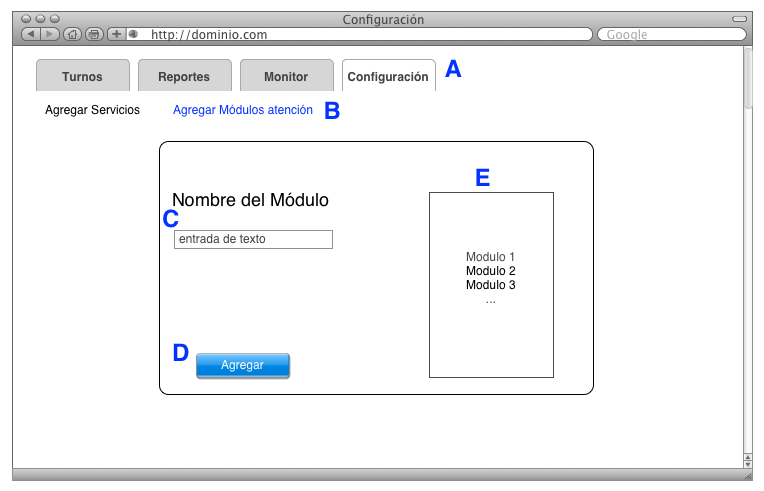
\includegraphics[scale=0.55]{images/capitulo4/mockupCU02.png}
\caption{\textit{Mockup} Caso de Uso 2 (CU02).}
\label{mockupCU01}
\end{figure}

\begin{spacing}{1.0}
	\begin{table}[H]
		\centering
		\caption{Caso de uso Real ``Seleccionar Servicio''.} 
		\begin{tabular}{| >{\arraybackslash\columncolor{gray!30}}p{3.1cm}| >{\arraybackslash}p{10.4cm}|}
			\hline 
			\rowcolor{gray!30} &\\[-0.2cm]
			\rowcolor{gray!30} \textbf{Caso de uso:} & \textbf{Seleccionar Servicio (CU03).} \\[0.2cm]
			\hline
			&\\[-0.2cm]
			\textbf{Actores:} & Cliente. \\[0.2cm]
			\hline
			&\\[-0.2cm]
			\textbf{Propósito:} & Obtener un turno de atención. \\[0.2cm]
			\hline
			&\\[-0.2cm]
			\textbf{Resumen:} & El usuario se abre la aplicación \textbf{Mi Turno} y presiona un servicio, mostrado en la pantalla principal, para obtener un turno de atención. \\[0.2cm]
			\hline
			&\\[-0.2cm]
			\textbf{Tipo:} & Primario y esencial. \\[0.2cm]
			\hline
			&\\[-0.2cm]
			\textbf{Precondiciones:} & {\tiny$\blacksquare$} El dispositivo móvil debe tener conexión a Internet. \\
			& {\tiny$\blacksquare$} La base de datos, servidor web y servidor central deben estar operativos. \\ [0.2cm]
			\hline
			\multicolumn{2}{| >{\arraybackslash\columncolor{gray!30}}c|}{}\\[-0.2cm]
			\multicolumn{2}{| >{\arraybackslash\columncolor{gray!30}}c|}{\textbf{Curso normal de los eventos}}\\[0.2cm]
		\end{tabular}
		
		\vspace{-0.5cm}
		\begin{center}
			\begin{tabular}{| >{\arraybackslash}p{6.75cm} | >{\arraybackslash}p{6.75cm} |}
				\hline
				\rowcolor{gray!30} &\\[-0.2cm]
				\rowcolor{gray!30} \textbf{Acción de los actores} & \textbf{Respuesta del sistema}\\[0.2cm]
				\hline
				&\\[-0.2cm]
				\textbf{1.} Este caso de uso comienza cuando un Cliente se acerca a un centro de atención y, desea obtener un turno para realizar un trámite en algún servicio del centro de atención. & \\
				\textbf{2.} El Cliente presiona un botón correspondiente al servicio que desea \textbf{(A)}. &\\
				& \textbf{3.} Muestra un cuadro de diálogo donde pregunta \textbf{¿Desea obtener ticket de atención?} \textbf{(B)}. \\
				\textbf{4.} El Cliente en caso que desee ese servicio presiona el botón \textbf{SI} \textbf{(C)}.  \\
				& \textbf{5.} Muestra un mensaje confirmando la acción. \\
				&\textbf{6.} Muestra una nueva pantalla donde se indica el \textbf{Turno} y \textbf{Servicio} \textbf{(D)}. \\
				\hline
				\multicolumn{2}{| >{\arraybackslash\columncolor{gray!30}}c|}{}\\[-0.2cm]
				\multicolumn{2}{| >{\arraybackslash\columncolor{gray!30}}c|}{\textbf{Cursos alternativos}}\\[0.2cm]
				\hline
				\multicolumn{2}{|l|}{}\\[-0.2cm]
				\multicolumn{2}{|l|}{\textbf{4.} El Cliente presionó equivocadamente el servicio y presiona el botón \textbf{NO}.}\\
				\multicolumn{2}{|l|}{\textbf{5.} El dispositivo móvil pierde comunicación con el servidor central.}\\
			\end{tabular}
		\end{center}
		
		\vspace{-0.5cm}
		\begin{tabular}{| >{\arraybackslash\columncolor{gray!30}}p{3.1cm}| >{\arraybackslash}p{10.4cm}|}
			\hline
			&\\[-0.2cm]
			\textbf{Post condiciones:} & La aplicación móvil queda trabajando en segundo plano a la espera de recibir Notificaciones. \\[0.2cm]
			\hline
		\end{tabular}
		
		\label{tabla_CU03}
	\end{table}
\end{spacing}

\begin{figure}[H]
\centering
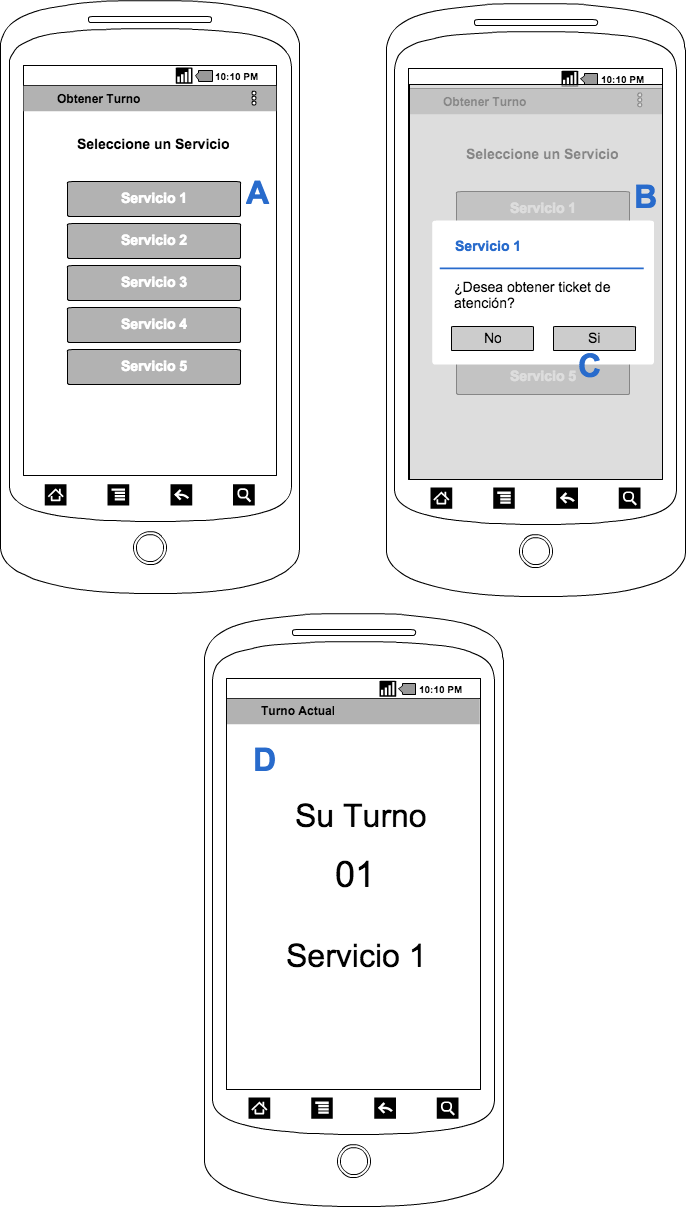
\includegraphics[scale=0.40]{images/capitulo4/mockupCU03.png}
\caption{\textit{Mockup} Caso de Uso 3 (CU03).}
\label{mockupCU03}
\end{figure}


\subsubsection{Diagramas de Secuencia}

\begin{figure}[H]
\centering
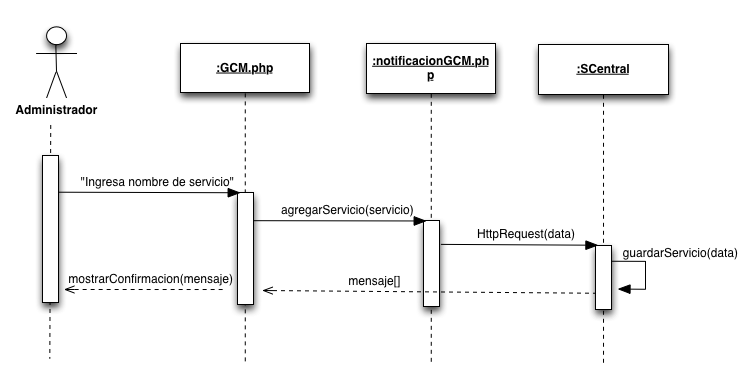
\includegraphics[scale=0.65]{images/capitulo4/dsAgregarServicio.png}
\caption{Diagrama de Secuencia Caso de Uso Agregar Servicios.}
\label{dsCUAS}
\end{figure}

\begin{figure}[H]
\centering
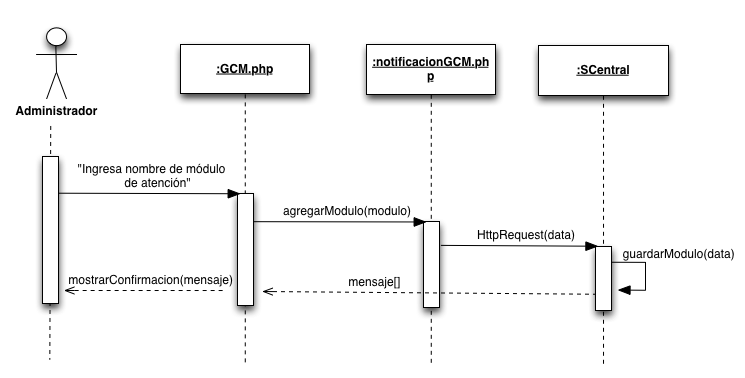
\includegraphics[scale=0.65]{images/capitulo4/dsAgregarModulo.png}
\caption{Diagrama de Secuencia Caso de Uso Agregar Módulo Atención.}
\label{dsCUAMA}
\end{figure}

\begin{figure}[H]
\centering
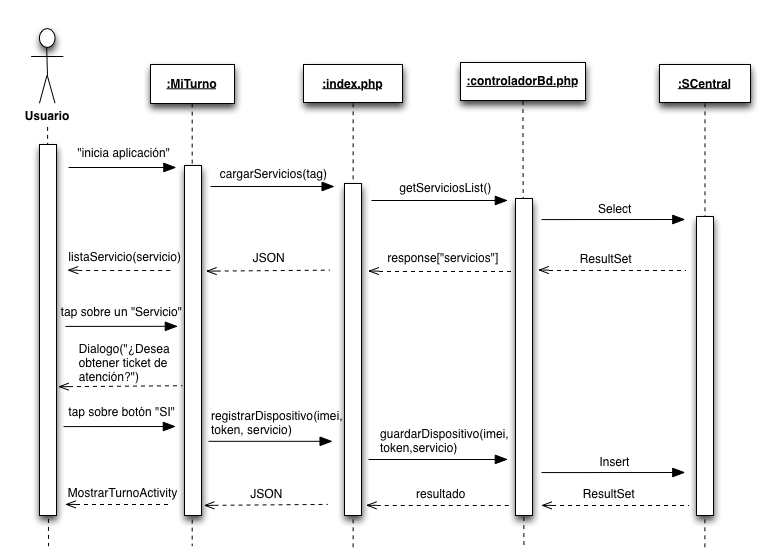
\includegraphics[scale=0.60]{images/capitulo4/dsSeleccionarServicio.png}
\caption{Diagrama de Secuencia Caso de Uso Seleccionar Servicio.}
\label{dsCUSS}
\end{figure}

\subsubsection{Diagrama de Clases}

\begin{figure}[H]
\centering
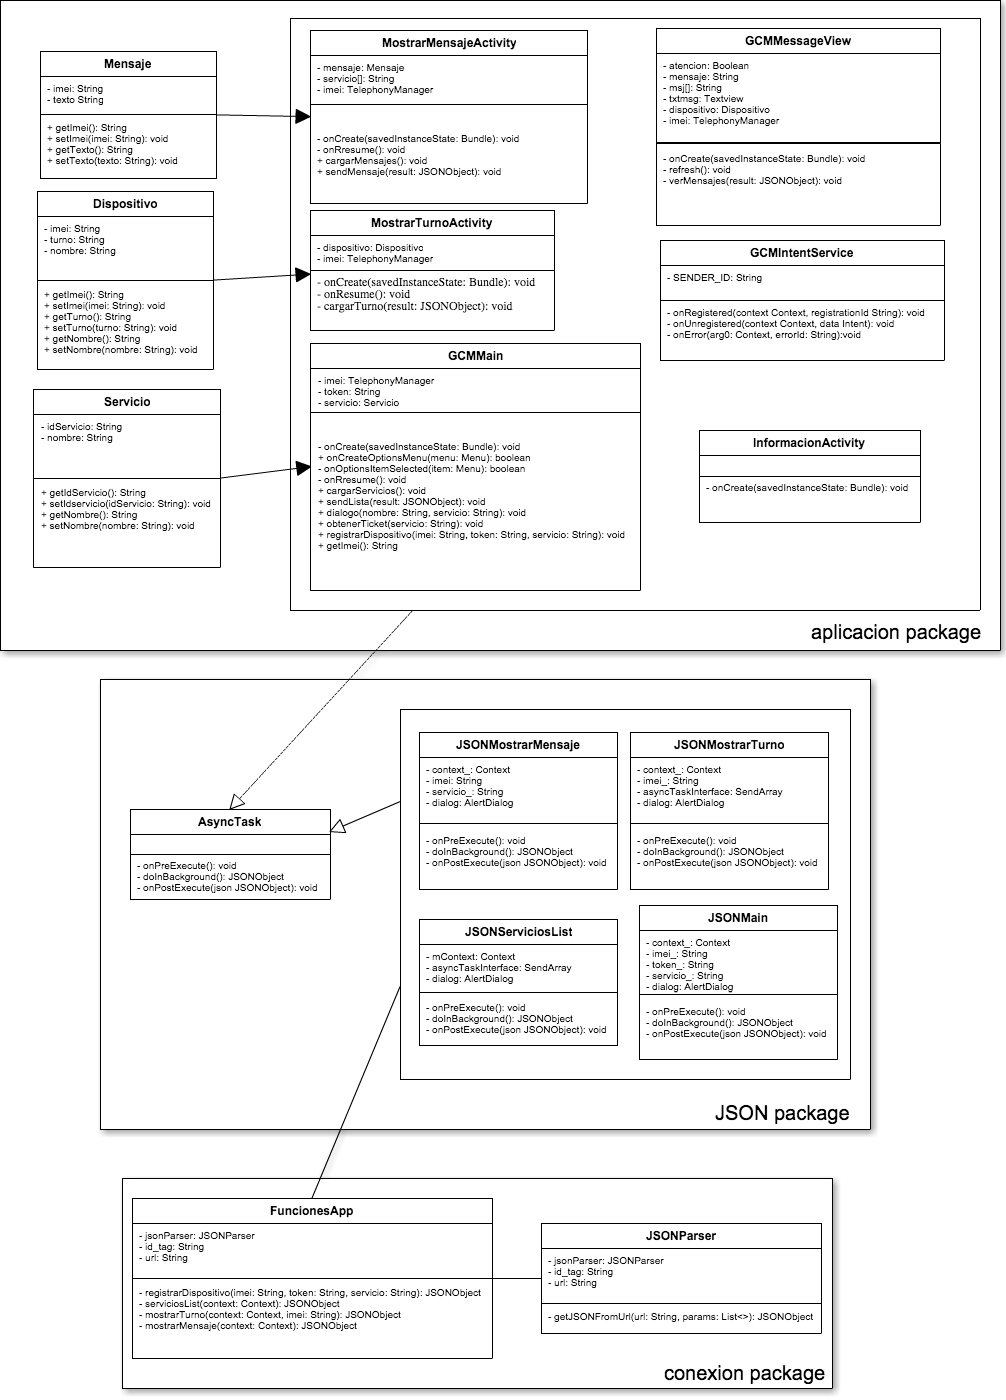
\includegraphics[scale=0.45]{images/capitulo4/diagramaClases.png}
\caption{Diagrama de Clases Aplicación Móvil.}
\label{diagramaClases}
\end{figure}

\subsubsection{Diagrama de Procesos}

\begin{figure}[H]
\centering
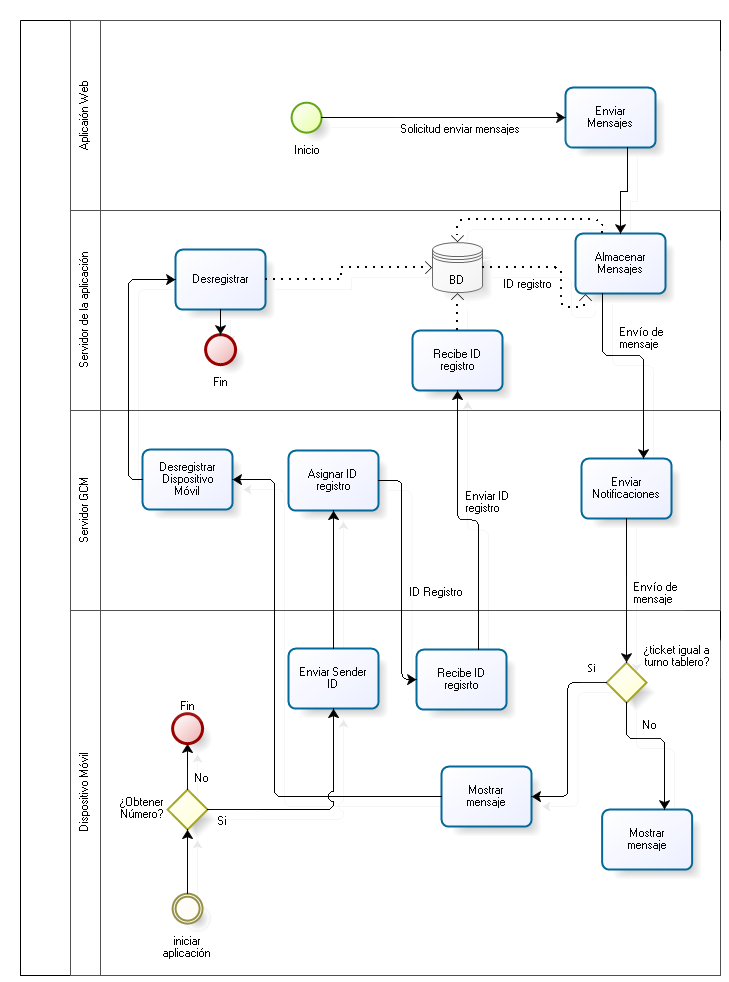
\includegraphics[scale=0.70]{images/capitulo4/diagramaProceso.png}
\caption{Diagrama de Proceso Aplicación Móvil.}
\label{diagramaProceso}
\end{figure}


\subsubsection{Modelo de Datos}

\begin{figure}[H]
\centering
\setlength\fboxsep{0pt}
\setlength\fboxrule{0.5pt}
\fbox{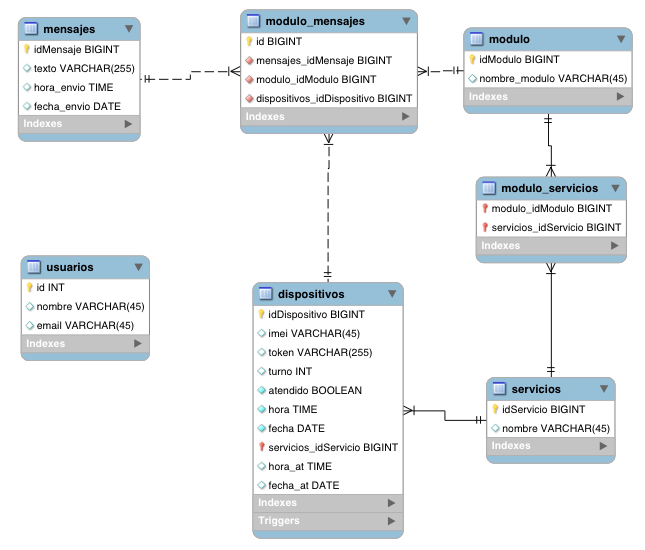
\includegraphics[scale=0.60]{images/capitulo4/modeloDatos.png}}
\caption{Modelo de datos.}
\label{modeloDeDatos}
\end{figure}

\myparagraph{Diccionario de datos}

\begin{spacing}{1.0}
	\begin{table}[H]
		\centering
		\caption{Diccionario de datos tabla ``dispositivos''.} 
		\begin{tabular}{|c|c|c|}
			\hline 
			\rowcolor{gray!30} &&\\
			\rowcolor{gray!30} \textbf{Columna} & \textbf{Tipo de dato} & \textbf{Descripción} \\ 
			\rowcolor{gray!30} &&\\
			\hline 
			&&\\[-0.2cm]
			idDispositivos & BIGINT & Identificador único de cada dispositivo. \\
			\hline 
			&&\\[-0.2cm]
			imei & VARCHAR(45) & Identificador propio de cada \textit{smartphone}. \\
			\hline 
			&&\\[-0.2cm]
			token & VARCHAR(255) & Identificador entregado por GCM a cada \\
			 & & dispositivo móvil registrado en el sistema. \\
			\hline 
			&&\\[-0.2cm]
			turno & INT & Número de turno de atención asignado \\
			 & & por el sistema a un dispositivo móvil. \\
			\hline 
			&&\\[-0.2cm]
			atendido & BOOLEAN & Estado de atención en que encuentra \\
			 & & un dispositivo, TRUE o FALSE. \\
			\hline 
			&&\\[-0.2cm]
			hora & TIME & Hora en que el dispositivo solicita un turno \\
			 & & de atención. \\
			\hline
			&&\\[-0.2cm]
			fecha & DATE & Fecha en que el dispositivo solicita un turno \\
			 & & de atención. \\
			\hline
			&&\\[-0.2cm]
			servicios\_idServicio & BIGINT & Clave foránea de la tabla servicios. \\
			\hline
			&&\\[-0.2cm]
			hora\_at & TIME & Hora en que el cliente es llamado para ser \\
			 & & atendido en un módulo de atención. \\
			\hline
			&&\\[-0.2cm]
			fecha\_at & DATE & Fecha en que el cliente es llamado \\
			 & & para ser atendido en un módulo de atención. \\
		    \hline
		\end{tabular}
		\label{diccionario_dispositivos}
	\end{table}
\end{spacing}

\begin{spacing}{1.0}
	\begin{table}[H]
		\centering
		\caption{Diccionario de datos tabla ``mensajes''.} 
		\begin{tabular}{|c|c|c|}
			\hline 
			\rowcolor{gray!30} &&\\
			\rowcolor{gray!30} \textbf{Columna} & \textbf{Tipo de dato} & \textbf{Descripción} \\ 
			\rowcolor{gray!30} &&\\
			\hline 
			&&\\[-0.2cm]
			idMensaje & BIGINT & Identificador único de cada mensaje. \\
			\hline 
			&&\\[-0.2cm]
			texto & VARCHAR(255) & Mensaje enviado desde el sistema \\
			 & & a cada \textit{smartphone}. \\
			\hline 
			&&\\[-0.2cm]
			hora\_envio & TIME & Hora en que se envió el mensaje. \\
			\hline 
			&&\\[-0.2cm]
			fecha\_envio & DATE & Fecha en que se envió el mensaje. \\
			\hline
		\end{tabular}
		\label{diccionario_mensajes}
	\end{table}
\end{spacing}

\begin{spacing}{1.0}
	\begin{table}[H]
		\centering
		\caption{Diccionario de datos tabla ``modulo''.} 
		\begin{tabular}{|c|c|c|}
			\hline 
			\rowcolor{gray!30} &&\\
			\rowcolor{gray!30} \textbf{Columna} & \textbf{Tipo de dato} & \textbf{Descripción} \\ 
			\rowcolor{gray!30} &&\\
			\hline 
			&&\\[-0.2cm]
			idModulo & BIGINT & Identificador único de cada \\
			 & & módulo de atención. \\
			\hline 
			&&\\[-0.2cm]
			nombre\_modulo & VARCHAR(45) & Nombre del módulo de atención. \\
			\hline 
		\end{tabular}
		\label{diccionario_modulo}
	\end{table}
\end{spacing}

\begin{spacing}{1.0}
	\begin{table}[H]
		\centering
		\caption{Diccionario de datos tabla ``servicios''.} 
		\begin{tabular}{|c|c|c|}
			\hline 
			\rowcolor{gray!30} &&\\
			\rowcolor{gray!30} \textbf{Columna} & \textbf{Tipo de dato} & \textbf{Descripción} \\ 
			\rowcolor{gray!30} &&\\
			\hline 
			&&\\[-0.2cm]
			idServicio & BIGINT & Identificador único de cada servicio. \\
			\hline 
			&&\\[-0.2cm]
			nombre & VARCHAR(45) & Nombre del servicio. \\
			\hline 
		\end{tabular}
		\label{diccionario_servicios}
	\end{table}
\end{spacing}

\begin{spacing}{1.0}
	\begin{table}[H]
		\centering
		\caption{Diccionario de datos tabla ``usuarios''.} 
		\begin{tabular}{|c|c|c|}
			\hline 
			\rowcolor{gray!30} &&\\
			\rowcolor{gray!30} \textbf{Columna} & \textbf{Tipo de dato} & \textbf{Descripción} \\ 
			\rowcolor{gray!30} &&\\
			\hline 
			&&\\[-0.2cm]
			id & INT & Identificador único de cada usuario. \\
			\hline 
			&&\\[-0.2cm]
			nombre & VARCHAR(45) & Nombre y apellido del usuario. \\
			\hline
			&&\\[-0.2cm]
			email & VARCHAR(45) & Correo electrónico del usuario. \\
			\hline 
		\end{tabular}
		\label{diccionario_usuarios}
	\end{table}
\end{spacing}

\begin{spacing}{1.0}
	\begin{table}[H]
		\centering
		\caption{Diccionario de datos tabla ``modulo\_mensajes''.} 
		\begin{tabular}{|c|c|c|}
			\hline 
			\rowcolor{gray!30} &&\\
			\rowcolor{gray!30} \textbf{Columna} & \textbf{Tipo de dato} & \textbf{Descripción} \\ 
			\rowcolor{gray!30} &&\\
			\hline 
			&&\\[-0.2cm]
			id & BIGINT & Identificador único de la tabla. \\
			\hline 
			&&\\[-0.2cm]
			mensajes\_idMensaje & BIGINT & Identificador único de cada mensaje. \\
			\hline
			&&\\[-0.2cm]
			modulo\_idModulo & BIGINT & Identificador único de cada \\
			 & & módulo de atención. \\
			\hline
			&&\\[-0.2cm]
			dispositivos\_idDispositivos & BIGINT & Identificador único de cada dispositivo. \\
			\hline 
		\end{tabular}
		\label{diccionario_servicios}
	\end{table}
\end{spacing}

\begin{spacing}{1.0}
	\begin{table}[H]
		\centering
		\caption{Diccionario de datos tabla ``modulo\_servicios''.} 
		\begin{tabular}{|c|c|c|}
			\hline 
			\rowcolor{gray!30} &&\\
			\rowcolor{gray!30} \textbf{Columna} & \textbf{Tipo de dato} & \textbf{Descripción} \\ 
			\rowcolor{gray!30} &&\\
			\hline 
			&&\\[-0.2cm]
			modulo\_idModulo & Identificador único de cada \\
			 & & módulo de atención. \\
			\hline 
			&&\\[-0.2cm]
			servicios\_idServicios & BIGINT & Identificador único de cada servicio. \\
			\hline
		\end{tabular}
		\label{diccionario_servicios}
	\end{table}
\end{spacing}





\newpage
%----------------------------------------------------------
%----------------------------------------------------------
\section{IMPLEMENTACIÓN DEL PROTOTIPO}
\subsection{Configuración ambiente de desarrollo y problemas enfrentados}

Este capítulo describe las diferentes etapas por las que ha atravezado el desarrollo de este sistema hasta llegar a su última iteración. Se inicia con una breve reseña de los pasos previos al desarrollo, es decir, la instalación de herramientas y configuración de la máquina de trabajo donde se desarrollaró la aplicación móvil y web. Luego, a modo de introducción, se da paso a la presentación de una aplicación básica utilizando el IDE \textit{Android Studio}, posteriormente se muestran los cuatro prototipos del sistema señidos a la metodología de desarrollo de \textit{software} elegida.\\

Las características del equipo de trabajo y dispositivo móvil para la realización y pruebas del sistema fueron:

\begin{itemize}
\item \textit{Notebook MacBook Pro}, procesador 2,5 Ghz \textit{Intel Core} i5.
\item \textit{Smartphone} Motorola Moto X, con Android 4.4.4.
\end{itemize}

Fue necesario instalar y activar algunos servicios que fueron escogidos para el proyecto. En la tabla 18 se indican las herramientas instaladas, activadas y/o servicios iniciados, junto con su versión, en la máquina de trabajo.

\begin{spacing}{1.0}
	\begin{table}[H]
		\centering
		\caption{Herramientas, estado y versión en máquina de trabajo.} 
		\begin{tabular}{|c|c|c|}
			\hline 
			\rowcolor{gray!30} &&\\
			\rowcolor{gray!30} \textbf{Herramienta} & \textbf{Acción requerida} & \textbf{Versión} \\ 
			\rowcolor{gray!30} &&\\
			\hline 
			&&\\[-0.2cm]
			Apache & Iniciar servicio & 2.4.9\\
			\hline 
			&&\\[-0.2cm]
			PHP & Activar servicio & 5.5.14 \\
			\hline 
			&&\\[-0.2cm]
			Android Studio & Descargar e instalar & 1.0 \\
			\hline 
			&&\\[-0.2cm]
			MySQL & Descargar, instalar e iniciar & 5.6.23 \\
			\hline 
			&&\\[-0.2cm]
			MySQLWorkbench & Descargar e instalar & 6.1 \\
			\hline			
		\end{tabular}
		\label{ambienteDesarrollo}
	\end{table}
\end{spacing}

Las herramientas que requerieren ser iniciadas y activadas vienen instaladas previamente en el Sistema Operativo. En cambio, las herramientas que no están incluidas fueron descargadas de su propio sitio web e instaladas posteriormente.\\ 

Durante instalación de las herramientas mencionadas no hubo mayores problemas; sin embargo, en los servicios, expuestos en la tabla anterior, se activaron e iniciaron mediante el uso de comandos a través del terminal de OS X. 

Para iniciar Apache, abrir el terminal e ingresar en modo super usuario, \textit{root}, para tener todos los permisos. En la Figura 22 se exhiben los comandos:

\begin{figure}[H]
\centering
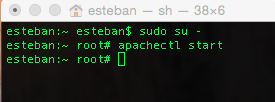
\includegraphics[scale=0.90]{images/capitulo5/apacheStart.png}
\caption{Iniciar Apache desde el terminal de OS X.}
\label{apacheStart}
\end{figure} 

Seguido de lo anterior, es recomendable corroborar que se ha iniciado Apache. Para ello, abrir el navegador web y en la barra de direcciones escribir: 'http://localhost', debe aparecer el mensaje 'It works!' como muestra la Figura 23.\\

\begin{figure}[H]
\centering
\setlength\fboxsep{0pt}
\setlength\fboxrule{0.5pt}
\fbox{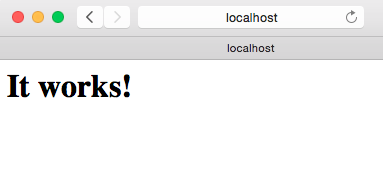
\includegraphics[scale=0.80]{images/capitulo5/localhost.png}}
\caption{Servicio Apache funcionando correctamente.}
\label{localhost}
\end{figure}

Posteriormente, se continúa con la activación de PHP. Nuevamente usando el terminal, dirigirse a la carpeta apache2: 'cd /etc/apache2/'. En esa carpeta se encuentra el archivo 'http.conf', dentro del archivo descomentar, borrar el signo '\#', la siguiente línea: 'LoadModule php5\_module libexec/apache2/libphp5.so'. Por último reiniciar Apache: 'apachectl restart'. Las figuras 24, 25 y 26 muestran lo descrito anteriormente.\\

\begin{figure}[H]
\centering
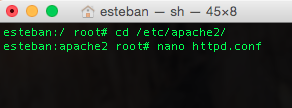
\includegraphics[scale=0.80]{images/capitulo5/httpd.png}
\caption{Acceso a carpeta apache2 y edición archivo httpd.conf.}
\label{activacionPHP}
\end{figure}

\begin{figure}[H]
\centering
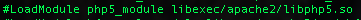
\includegraphics[scale=0.80]{images/capitulo5/libphp.png}
\caption{Habilitar PHP para Apache.}
\label{libphp}
\end{figure}

\begin{figure}[H]
\centering
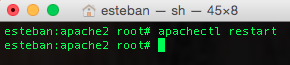
\includegraphics[scale=0.80]{images/capitulo5/apacheRestart.png}
\caption{Reiniciando Apache.}
\label{apacheRestart}
\end{figure}

Para finalizar, es importante aclarar que MySQLWorkbench\footnote{Es una herramienta visual de diseño, administración, creación y mantención de bases de datos MySQL. Más información en: \url{http://www.mysql.com/products/workbench/}}, Android Studio\footnote{\url{http://developer.android.com/sdk/index.html}} y MySQL\footnote{\url{http://dev.mysql.com/downloads/mysql/}} fueron descargados e instalados sin inconvenientes.\\

\subsection{Presentación de prototipos}

En esta sección, se muestra el crecimiento y nuevas funciones que ha logrado el sistema en las diferentes iteraciones. En cada caso se entrega una explicación de los aspectos que se consideran más importantes, y que forman parte de situaciones que exigieron interiorizarse para superar inidencias que surgieron en algunas de las etapas que se enseñan en los siguientes puntos.\\

\subsubsection{Prototipo 1: Aplicación básica en android Studio}

La primera aplicación se realizará a modo de ejercicio para corroborar que está funcionando correctamente \textit{Android Studio} y el \textit{smartphone}, para probar las aplicaciones hechas. Antes de realizar alguna acción es necesario tener el celular en modo depuración. Para esto hay que dirigirse a: Configurar -> Programador -> Depuración por USB. La Figura 27 muestra la opción que debe estar seleccionada.\\

\begin{figure}[H]
\centering
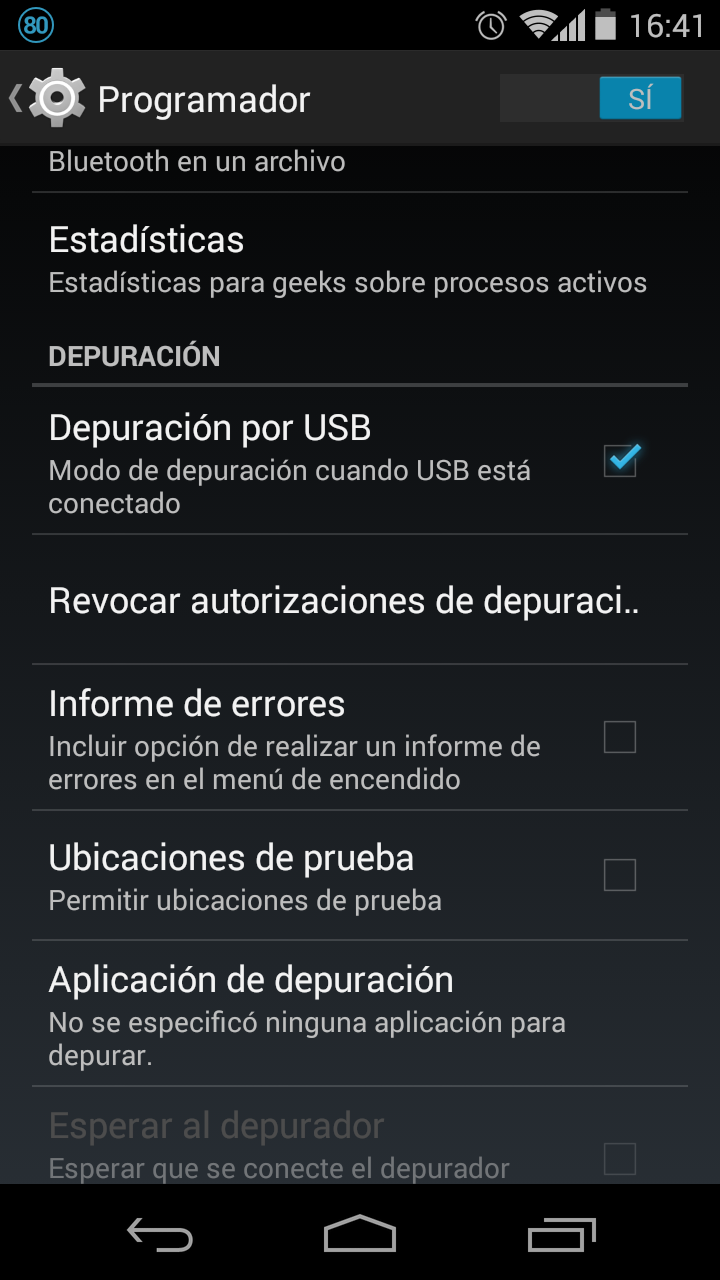
\includegraphics[scale=0.25]{images/capitulo5/modoDepuracion.png}
\caption{Modo Depuración por USB activado en \textit{Android} 4.4.4.}
\label{modoDepuracion}
\end{figure}

En la Figura 28, se puede apreciar la ventana de bienvenida de \textit{Android Studio}. Aquí es posible crear nuevos proyectos, abrir proyectos existentes, entre otras funciones.\\

\begin{figure}[H]
\centering
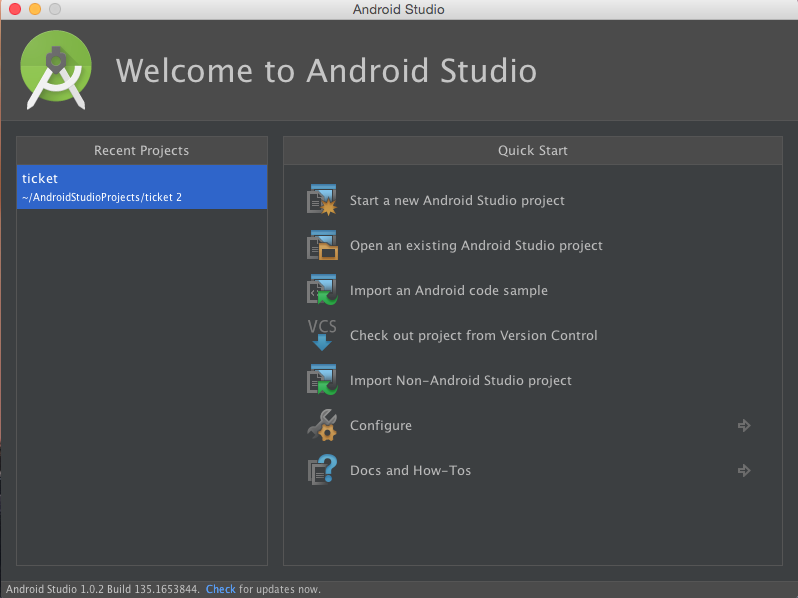
\includegraphics[scale=0.40]{images/capitulo5/androidStudio.png}
\caption{Ventana bienvenida \textit{Android Studio}.}
\label{androidStudio}
\end{figure}

En el momento que se crea un nuevo proyecto, luego de ingresar el nombre que éste tendrá, el asistente solicita elegir la versión mínima sobre la cual correrá nuestra aplicación móvil. Por lo tanto, es importante elegir correctamente, para evitar futuras complicaciones de compatibilidad cuando se cargue la aplicación en equipos que, posiblemente, tengan una versión menor a la elegida. En el menú desplegable de la Figura 29 se debe elegir una versión de API que será la versión mínima que necesitará la aplicación para ejecutarse en un \textit{smartphone}. La versión más antigua disponible en el menú es \textit{Android} 4.0.3 - \textit{IceCreamSandwich} y la más nueva es la versión reciente \textit{Android} 5.0 - \textit{Lollipop}.\\

\begin{figure}[H]
\centering
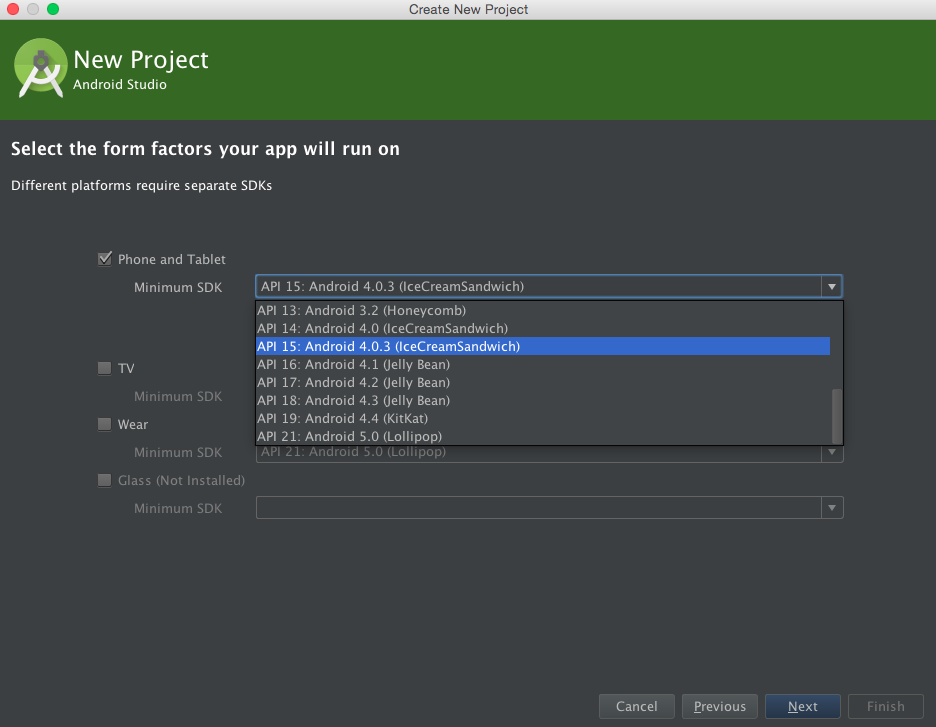
\includegraphics[scale=0.40]{images/capitulo5/minSDK.png}
\caption{Elección de API mínima requerida.}
\label{minSDK}
\end{figure}

El proyecto en el entorno de desarrollo, Figura 30, a la izquierda cuenta con un árbol para navegar y acceder a las diversas carpetas y archivos que contiene la aplicación. El código fuente de nuestro programa \textit{Android}, \textbf{controlador}, se encuentra dentro de la carpeta: app -> src -> main -> java. Es ahí donde se encuentran las clases del proyecto que dan vida a la interfaz gráfica de la aplicación, que en el patrón MVC corresponde a la \textbf{vista}. Ésta última, dentro del proyecto la ubicamos en la ruta: app -> src -> main -> res -> layout. Acá están almacenadas todas las pantallas que tendrá nuestra aplicación. A la derecha de la venta en la Figura 30 se aprecia el código fuente de la aplicación básica realizada con fines de prueba.\\

\begin{figure}[H]
\centering
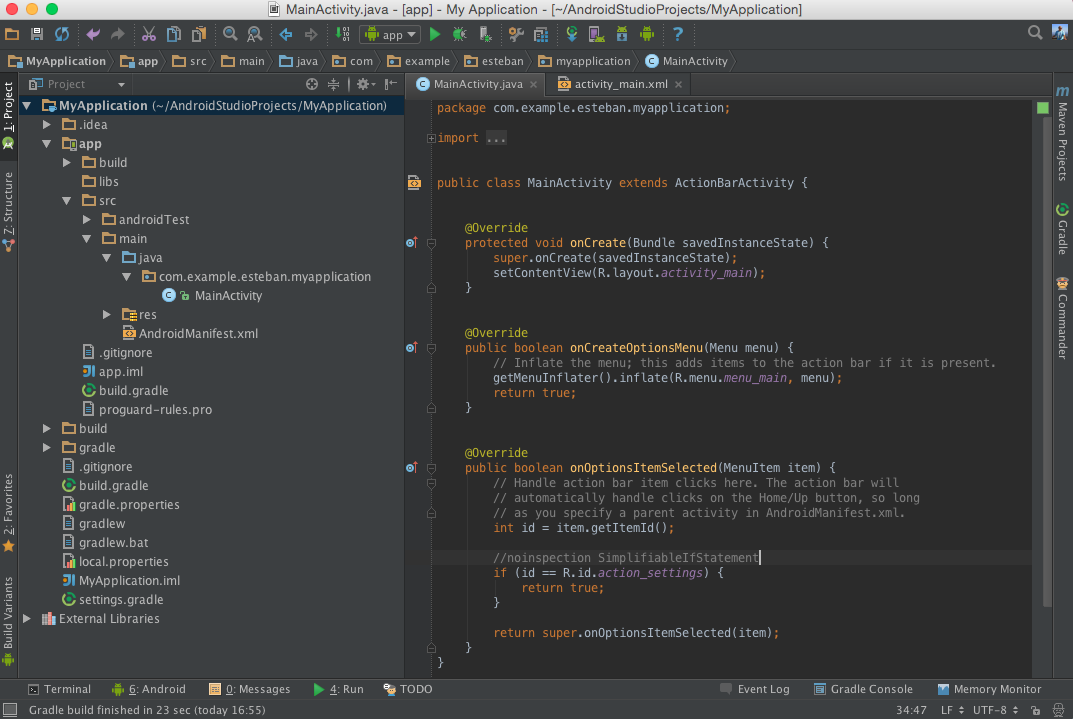
\includegraphics[scale=0.40]{images/capitulo5/proyectoAndroid.png}
\caption{Proyecto nuevo en \textit{Android Studio}.}
\label{proyectoAndroid}
\end{figure}

Luego de proceder a compilar el proyecto, y previamente haber conectado el celular al computador de trabajo, la aplicación móvil es enviada al smartphone a través del cable USB. Ya en el dispositivo ésta es instalada y ejecutada automáticamente. En la Figura 31 se ve el resultado del proyecto creado anteriormente. Debido a que no hubo inconvenientes en esta pequeña prueba, se concluye que el entorno de trabajo está listo para iniciar el desarrollo de la aplicación móvil, que forma parte del sistema propuesto como solución a la problemática antes definida en la sección 3.1 del documento.\\

\begin{figure}[H]
\centering
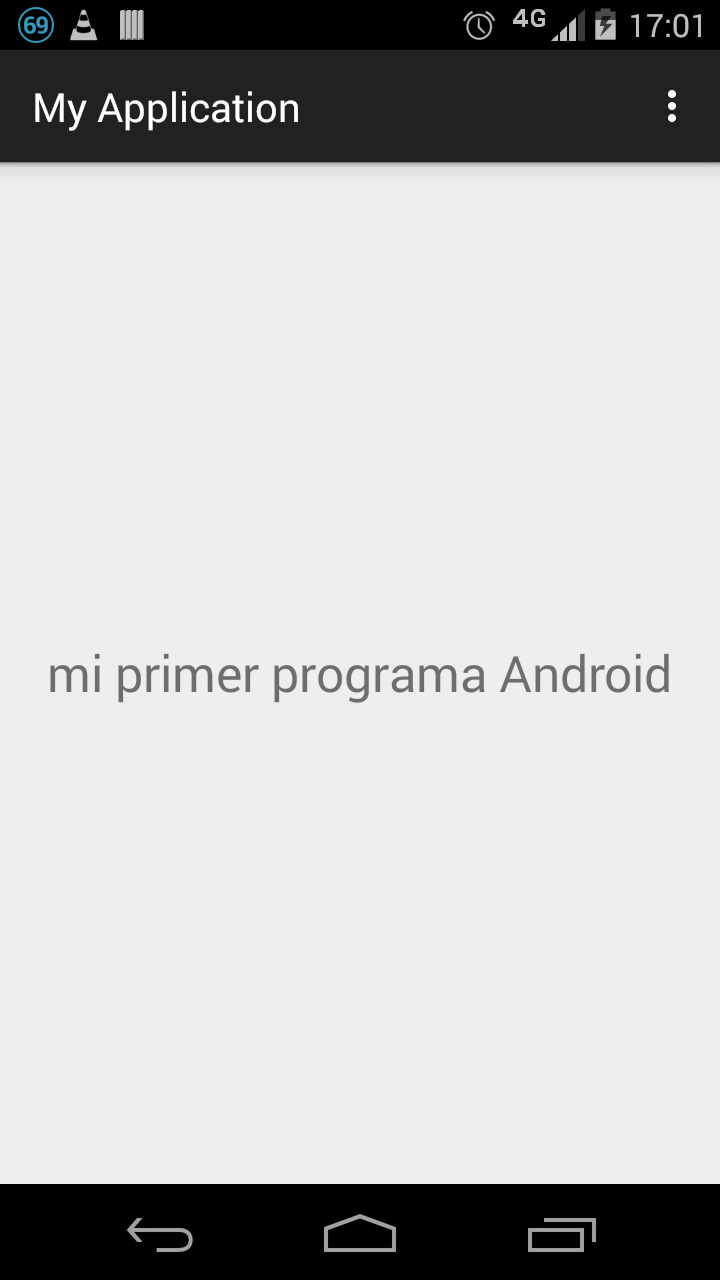
\includegraphics[scale=0.25]{images/capitulo5/primeraAplicacion.png}
\caption{Primera aplicación móvil de prueba.}
\label{minSDK}
\end{figure}

\subsubsection{Prototipo 2: Cliente y Servidor GCM}

En esta sección, se mostrará la implementación del servidor y cliente que envía y recibe mensajes, respectivamente, a través de \textit{Google Cloud Messaging}.\\  

\myparagraph{Cliente}

Antes de crear un proyecto en \textit{Android Studio} es necesario crear un proyecto, ver Figura 32, en \textit{Google Developers Console.\footnote{Es un espacio que tienen los desarrolladores de \textit{Google} para la gestión y visualización de las API de la compañía que sus proyectos utilizan. Más información en: \url{https://developers.google.com/console/help/new/}}}\\


\begin{figure}[H]
\centering
\setlength\fboxsep{0pt}
\setlength\fboxrule{0.5pt}
\fbox{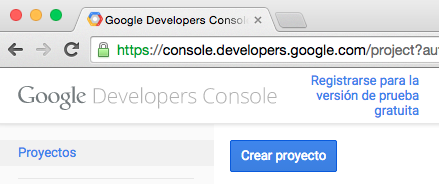
\includegraphics[scale=0.60]{images/capitulo5/gdc.png}}
\caption{Crear nuevo proyecto en Google Developers Console.}
\label{gdc}
\end{figure}

Luego de ser creado el proyecto, se desplega un resumen con información del proyecto (Figura 33), en la que aparece el \textit{PROJECT NUMBER} que corresponde a un identificador único de los proyectos creados en esta plataforma. Mas adelante será incluido en la aplicación móvil.\\

\begin{figure}[H]
\centering
\setlength\fboxsep{0pt}
\setlength\fboxrule{0.5pt}
\fbox{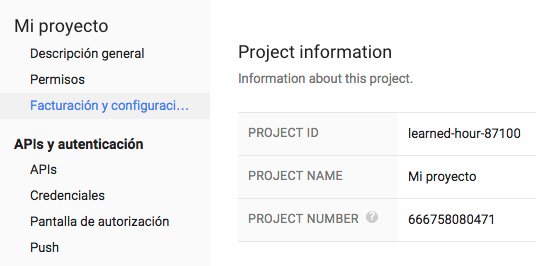
\includegraphics[scale=0.50]{images/capitulo5/resumenProyecto.png}}
\caption{Resumen proyecto.}
\label{resumenProyecto}
\end{figure}

Posteriormente es necesario habilitar APIs que provee \textit{Google} para los diferentes servicios que ofrece (\textit{Calendar, Contacts, Gmail, Google Maps Android, Google Play Game Services}, entre muchos servicios más.). Para efectos del proyecto sólo se habilitará la API \textit{Google Cloud Messaging for Android} que se puede apreciar en la Figura 34.\\

\begin{figure}[H]
\centering
\setlength\fboxsep{0pt}
\setlength\fboxrule{0.5pt}
\fbox{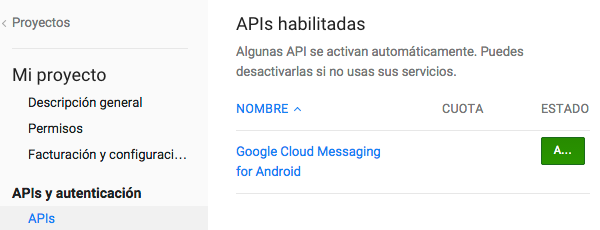
\includegraphics[scale=0.50]{images/capitulo5/API.png}}
\caption{Activación de API para proyecto.}
\label{API}
\end{figure}

Dentro de la API seleccionada, es importante crear una clave nueva para un servidor a través del cual circulan las notificaciones que sean enviadas desde el servidor del sistema. Ver Figuras 35, 36 y 37. En la Figura 38 se muestra un resumen con información a cerca del servidor creado. En la primera línea del resumen se encuentra la Clave DE LA API, que corresponde a un identificador único de dicho servidor. Este identificador al igual que el \textit{PROJECT NUMBER} serán incluidos en el sistema. \\

\begin{figure}[H]
\centering
\setlength\fboxsep{0pt}
\setlength\fboxrule{0.5pt}
\fbox{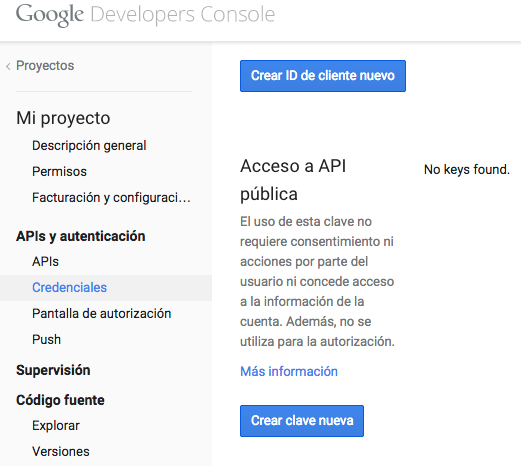
\includegraphics[scale=0.40]{images/capitulo5/claveNueva.png}}
\caption{Crear clave nueva.}
\label{cuentaNueva}
\end{figure}

\begin{figure}[H]
\centering
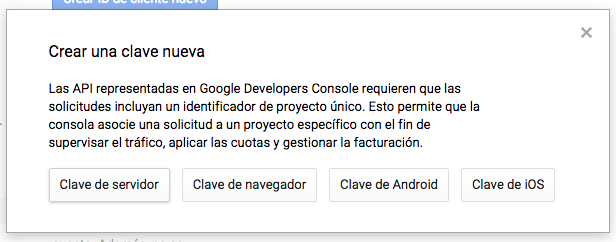
\includegraphics[scale=0.40]{images/capitulo5/cuentaNueva.png}
\caption{Crear clave nueva clave de servidor.}
\label{crearClaveNueva}
\end{figure}

\begin{figure}[H]
\centering
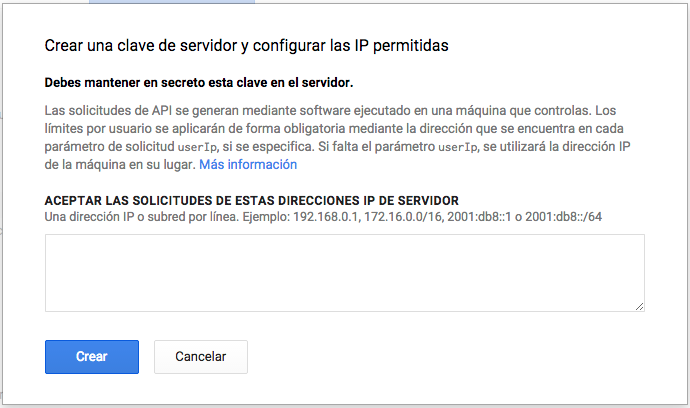
\includegraphics[scale=0.50]{images/capitulo5/crearClave.png}
\caption{Crear clave de servidor.}
\label{botonClaveNueva}
\end{figure}

\begin{figure}[H]
\centering
\setlength\fboxsep{0pt}
\setlength\fboxrule{0.5pt}
\fbox{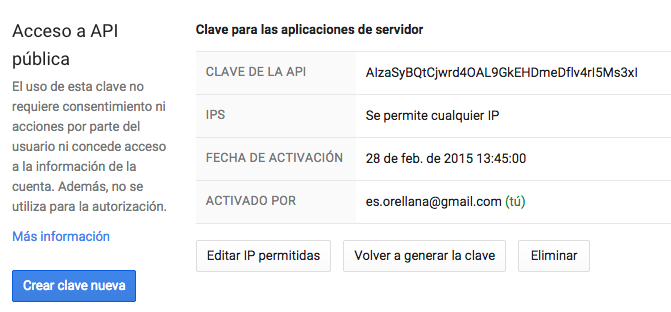
\includegraphics[scale=0.50]{images/capitulo5/resumenServidor.png}}
\caption{Resumen servidor.}
\label{resumenServidor}
\end{figure}

Dentro de \textit{Android Studio} en el \textit{SDK Manager} hay que instalar el \textit{package} de \textit{Google Play Services}, Figura 39, que contiene la libreria GCM.jar que debe ser agregada al proyecto  para que funcione la comunicación entre la aplicación \textit{Android} y los servidores de \textit{Google} desde donde vienen las notificaciones enviadas desde el servidor local.\\

\begin{figure}[H]
\centering
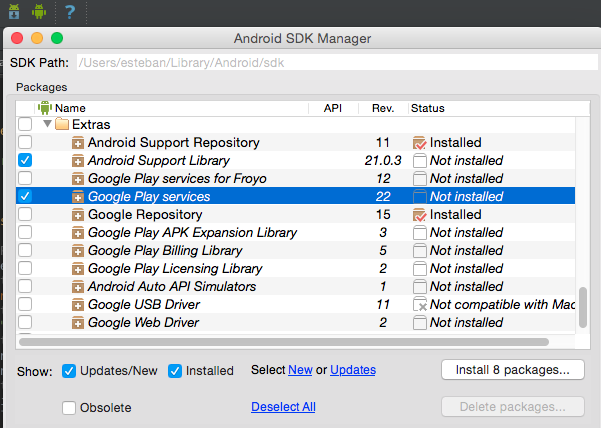
\includegraphics[scale=0.50]{images/capitulo5/sdkManager.png}
\caption{Instalación \textit{Google Play Services}.}
\label{sdkManager}
\end{figure}

En el proyecto de la aplicación cliente para \textit{Android} se tienen tres clases escritas en lenguaje java: GCMMainActivity, GCMIntentService y GCMMessageView. Entre todas se encargan de hacer posible: el registro del dispositivo. Es decir, solicitar un identificador único para el dispositivo móvil a los servidores de GCM y de esta forma poder recibir y visualizar las notificaciones. Lo anterior se muestra en la Figura 40.\\

\begin{figure}[H]
\centering
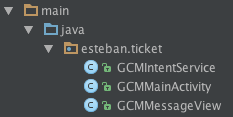
\includegraphics[scale=0.70]{images/capitulo5/proyecto.png}
\caption{Clases del proyecto.}
\label{clasesProyecto}
\end{figure}

Como se mencionó anteriormente, el \textit{PROJECT ID} sería incluido en el proyecto de \textit{Android Studio}, Figura 41. De no ser agregado este ID, la aplicación móvil queda incomunicada y sería imposible que reciba los mensajes, ya que 'no sabe' de qué proyecto debe 'escuchar' los mensajes.\\

\begin{figure}[H]
\centering
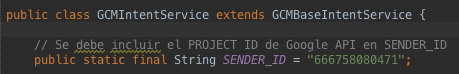
\includegraphics[scale=0.70]{images/capitulo5/idProyecto.png}
\caption{Incluir el \textit{PROJECT ID} en la aplicación.}
\label{idProyecto}
\end{figure}

La pantalla que se muestra en la Figura 42 corresponde a la aplicación creada, el botón 'Registrar Dispositivo' al ser presionado realiza la acción de solicitar el identificador asociado al dispositivo. Éste nuevo ID, sirve para asociar el celular al servidor de la API creados anteriormente. \\

\begin{figure}[H]
\centering
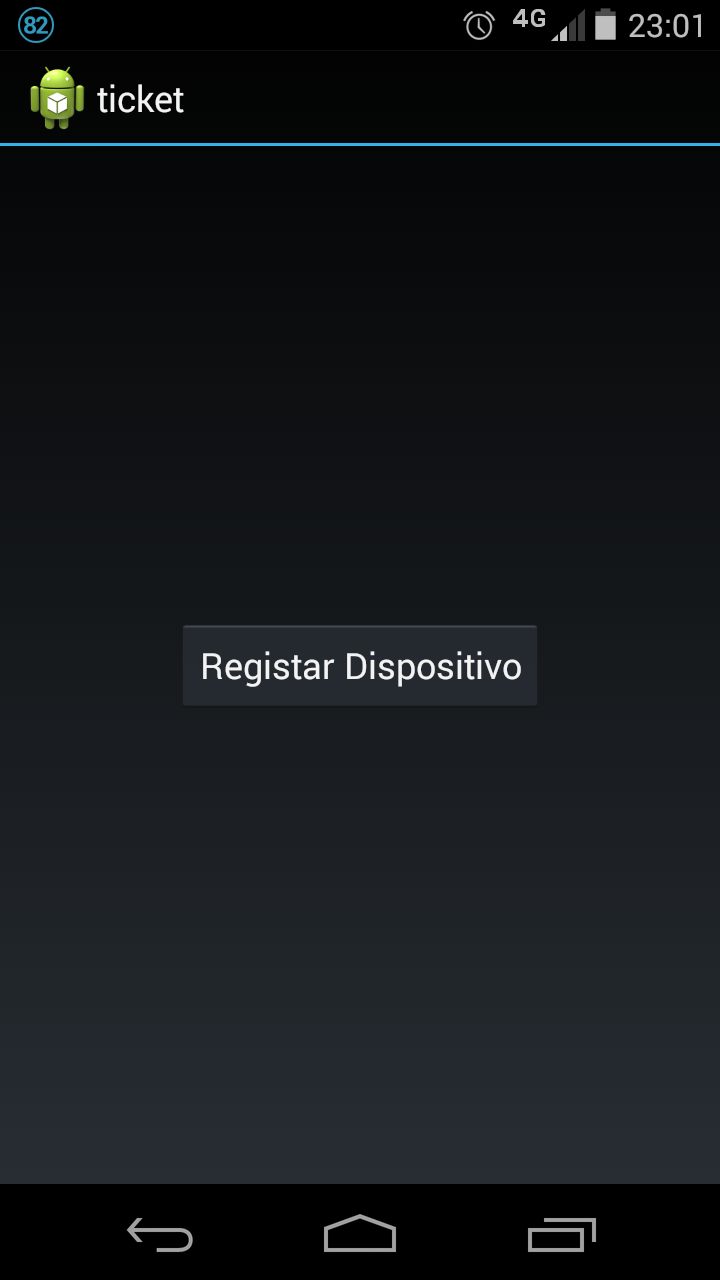
\includegraphics[scale=0.20]{images/capitulo5/registrarDispositivo.png}
\caption{Registrar dispositivo desde la aplicación.}
\label{registrarDispositivo}
\end{figure}

\myparagraph{Servidor}

El servidor está implementado en html y es la aplicación web que se mostró en las secciones anteriores. Su función es capturar datos en un formulario que posteriormente será enviado a una clase externa escrita en lenguaje PHP, la que se encarga de recibir los datos, encapsularlos y enviarlos al servidor de \textit{Google Cloud Messaging} que se creó anteriormente. En la Figuras siguientes: 43, 44 y 45 se muestra el código del mismo y después se expone el servidor en el navegador web.\\

\begin{figure}[H]
\centering
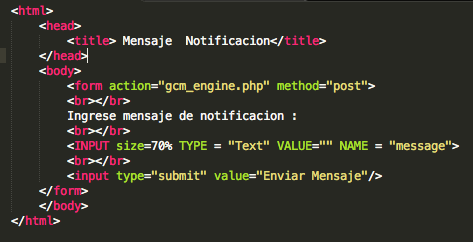
\includegraphics[scale=0.50]{images/capitulo5/codigoServidor.png}
\caption{Codigo html del Servidor.}
\label{codigoServidor}
\end{figure}

\begin{figure}[H]
\centering
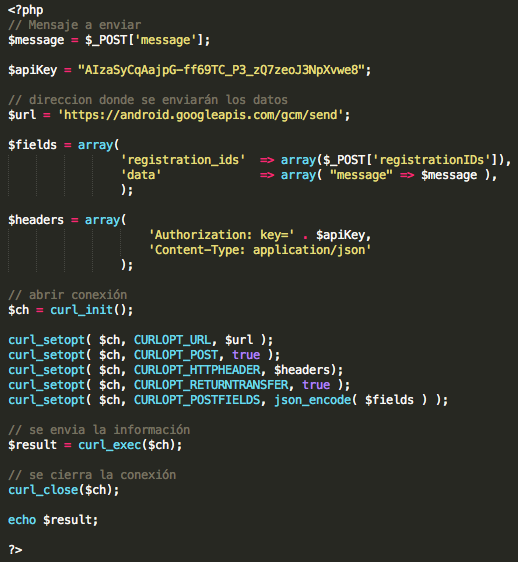
\includegraphics[scale=0.50]{images/capitulo5/codigoGCM.png}
\caption{Codigo clase gcm\_engine.php.}
\label{codigoPHP}
\end{figure}

\begin{figure}[H]
\centering
\setlength\fboxsep{0pt}
\setlength\fboxrule{0.5pt}
\fbox{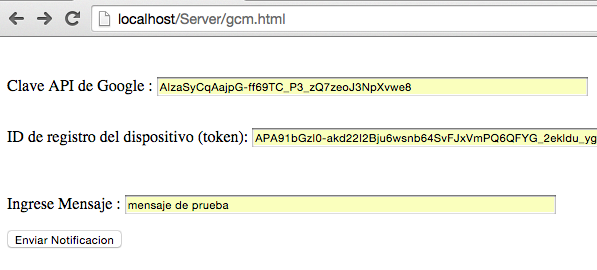
\includegraphics[scale=0.50]{images/capitulo5/servidor.png}}
\caption{Servidor.}
\label{servidor}
\end{figure}

En la Figura 45, el servidor tiene tres campos de texto. El primero, corresponde a la clave API del servidor de \textit{Google} antes creado y expuesto en la Figura 38. El segundo campo de texto, solicita que se ingrese el ID de registro del dispositivo. Éste es entregado, luego de presionar el botón 'Registrar Dispositivo' en la aplicación, ver Figura 42, por el servidor de la API creado en los pasos anteriores. En el tercer campo de texto, se debe ingresar el mensaje o notificación a enviar al o los dispositivos que tienen instalada la aplicación y se han registrado al presionar el botón antes mencionado. Por último, se debe presionar el boton 'Enviar Notificación' y el mensaje será enviado inmediatamente y podrá ser visualizado en el dispositivo móvil. Ver Figuras 46 y 47.\\

\begin{figure}[H]
\centering
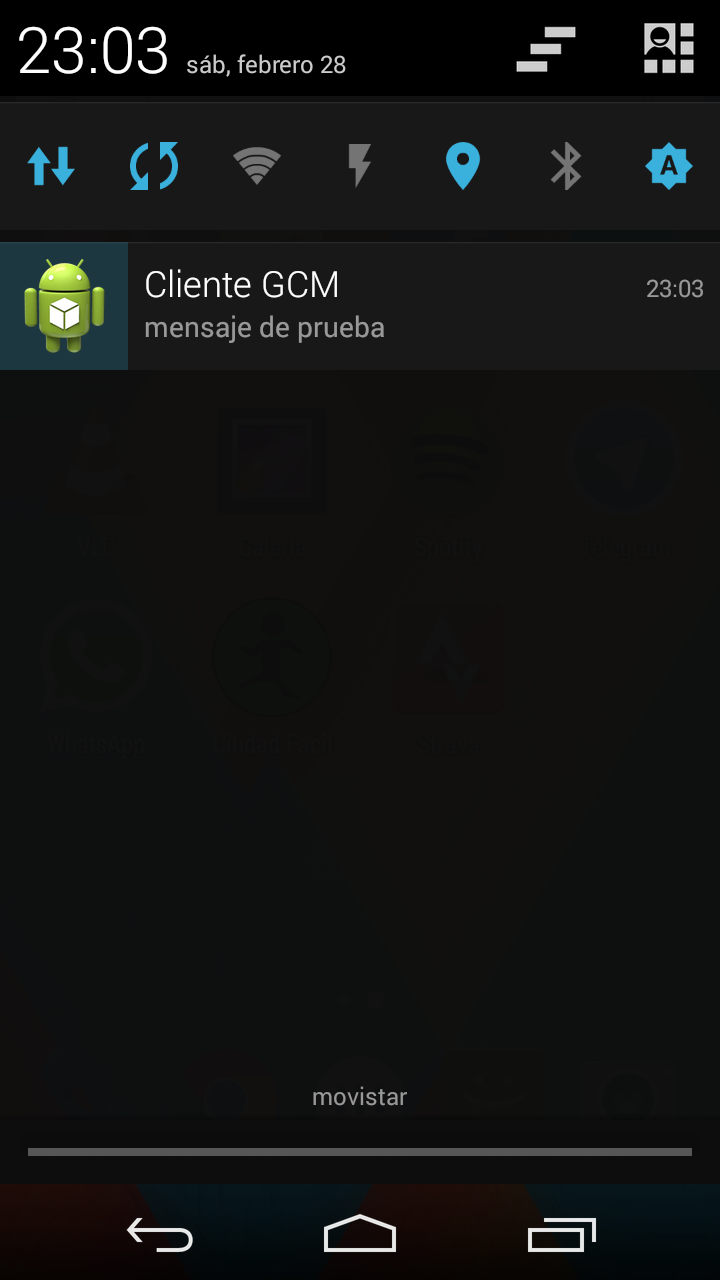
\includegraphics[scale=0.20]{images/capitulo5/notificacion.png}
\caption{Notificación \textit{Push} recibida.}
\label{notificacion}
\end{figure}

\begin{figure}[H]
\centering
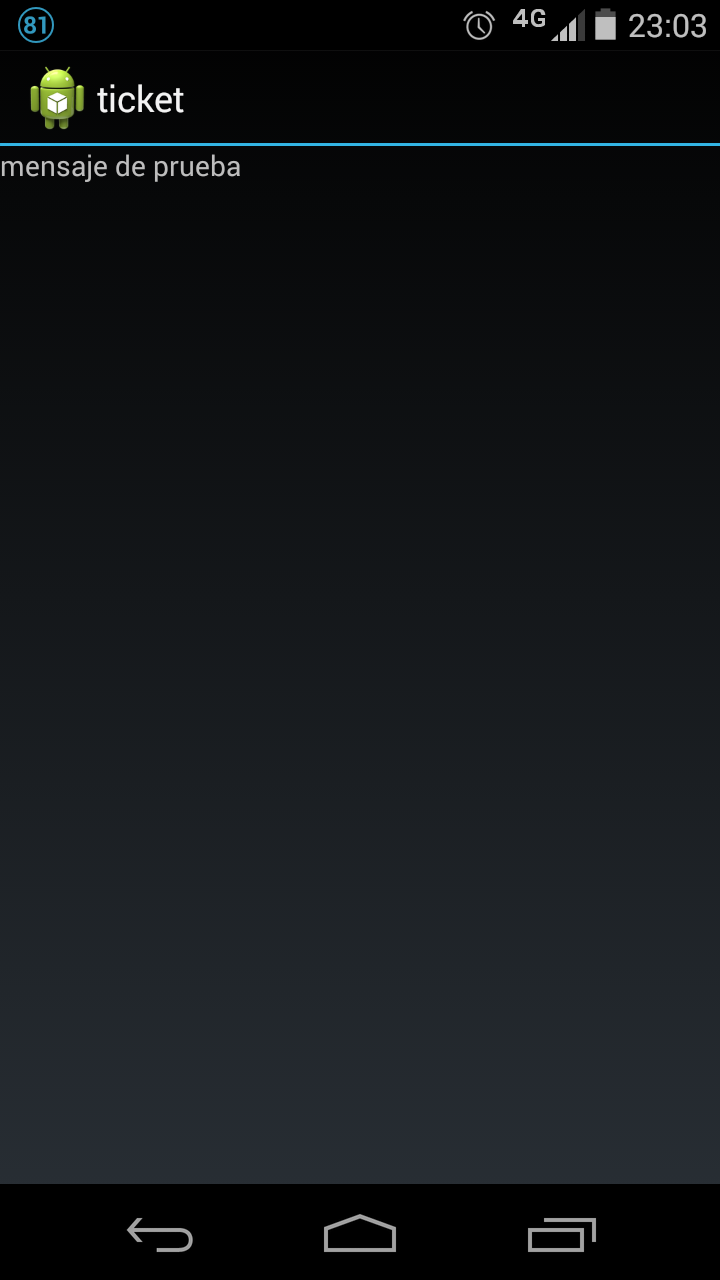
\includegraphics[scale=0.20]{images/capitulo5/notificacionApp.png}
\caption{Visualizacion contenido de notificación.}
\label{notificacionContenido}
\end{figure}

En este ítem se ha explicado paso por paso como se implementó este primer prototipo. Además, se resuelve una parte escencial de todo el sistema propuesto como solución a la problemática definida.\\

\subsubsection{Prototipo 3: Comunicar Android y MySQL}

Una forma de comunicar una aplicación \textit{Android} con una base de datos externa, que se encuentre en una máquina remota, es utilizando servicios web y un formato de intercambio de datos como es JSON\footnote{Estos conceptos y características fueron tratados con anterioridad en las secciones 2.1.4 y 3.4.2}. En la sección 2.1.4 - \textit{Web Service}, se explicó como el es flujo de datos entre: una aplicación \textit{Android} - PHP - MySQL.\\

Por el lado de la aplicación \textit{Android}, se agregaron funciones y clases al proyecto que realizan la tarea de capturar datos y enviarlos al servicio web 'index.php' ubicado en la estación de trabajo que a su vez juega el papel de servidor externo. En la Figura 48 se aprecia la misma pantalla de la aplicación pero, ahora el boton envía datos al servidor para que sean almacenados. Los datos que el celular envía a MySQL son: IMEI, clave API de \textit{Google} \textit{(token)}, lo anterior aparece en las Figuras 48, 49, 50 y 51.\\

\begin{figure}[H]
\centering
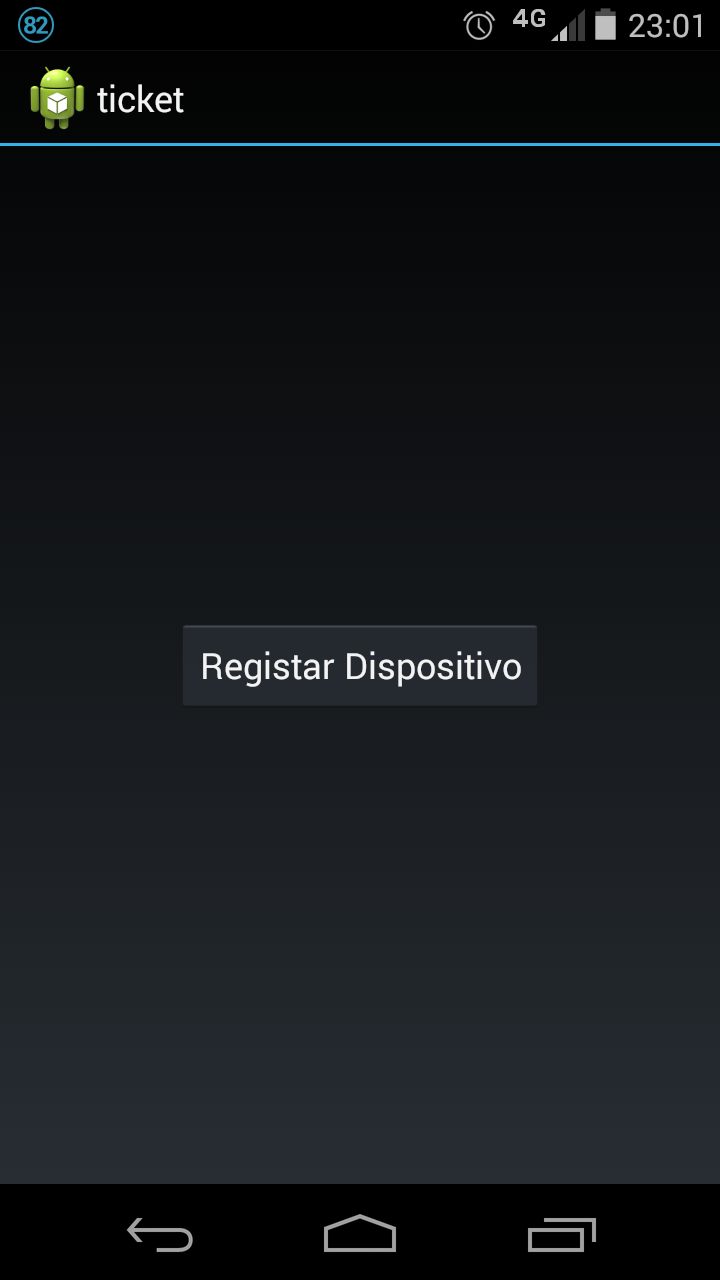
\includegraphics[scale=0.20]{images/capitulo5/registrarDispositivo.png}
\caption{Registrar dispositivo en MySQL.}
\label{registrarDispositivo}
\end{figure}

\begin{figure}[H]
\centering
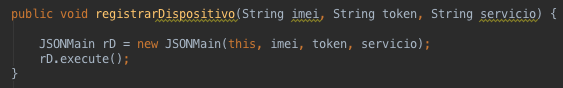
\includegraphics[scale=0.70]{images/capitulo5/funcionesAppRD.png}
\caption{Código de función registrar dispositivo.}
\label{registrarDispositivo}
\end{figure}

\begin{figure}[H]
\centering
\includegraphics[scale=0.70]{images/capitulo5/JSONMain.png}
\caption{Código clase asíncrona JSONMain.}
\label{registrarDispositivo}
\end{figure}

\begin{figure}[H]
\centering
\includegraphics[scale=0.70]{images/capitulo5/funcionRD.png}
\caption{Código de función registrarDispositivo() en clase FuncionesApp().}
\label{registrarDispositivo}
\end{figure}

Los datos cuando son enviados con JSON al servidor central llegan al webservice que tiene por nombre: index.php (en la Figura 51, se aprecia la variable 'url' que contiene la ubicación de éste.) y que a través del método POST recibe entre los datos una variable llamada 'tag' que sirve para discriminar que método debe ser utilizado dentro del mismo para realizar alguna tarea específica. Ver Figura 52.\\

\begin{figure}[H]
\centering
\includegraphics[scale=0.70]{images/capitulo5/index.png}
\caption{Porción de código de servicio web.}
\label{registrarDispositivo}
\end{figure}

En la Figura 52 se muestra que se realiza una instancia de la función 'guardarDispositivo()' y se le pasan como argumentos los datos enviados desde el dispositivo móvil para ser almacenados. Tal método, se encuentra en la clase PHP DB\_Functions.php. Esta clase se encarga de comunicarse directamente con la base de datos MySQL, ya sea para realizar una consulta, \textit{SELECT}, o guardar información, \textit{INSERT}. En la Figura 53 se puede ver la implementación de un \textit{INSERT} con la información recibida.\\

\begin{figure}[H]
\centering
\includegraphics[scale=0.60]{images/capitulo5/guardarDisp.png}
\caption{Código de función guardarDispositivos() en clase DB\_Functions.PHP.}
\label{registrarDispositivo}
\end{figure}

Se puede ver en la Figura 54 que los datos han sido almacenados correctamente en la base de datos que se encuentra en el servidor central.\\

\begin{figure}[H]
\centering
\setlength\fboxsep{0pt}
\setlength\fboxrule{0.5pt}
\fbox{\includegraphics[scale=0.80]{images/capitulo5/MySQL.png}}
\caption{Datos almacenados correctamente en MySQL.}
\label{registrarDispositivo}
\end{figure}


\subsection{Solución final}

la solución final es el resultado de la cuarta y última iteración del proyecto, de acuerdo al ciclo de vida elegido. Así como fueron descritos anteriormente los prototipos, a continuación en este apartado se describirán las diferentes partes que forman el sistema y sus características.

\subsubsection{Servidor central}

El servidor central contiene los servicios que actuan como orquestadores del sistema definitivo. Aquí se encuentra la base de datos MySQL, el servicio web (index.php) y la aplicación web (GCM.php).\\ 

\subsubsection{Monitor}

El monitor del sistema tiene por objetivo mostrar los dos últimos números que están siendo atendidos en servicios distintos. Esta pantalla estará ubicada en un televisor ubicado en una zona visible para que los clientes puedan visualizar la información. Se actualiza cuando un número es llamado al módulo de atención. La Figura 55 muestra lo mencionado.

\begin{figure}[H]
\centering
\setlength\fboxsep{0pt}
\setlength\fboxrule{0.5pt}
\fbox{\includegraphics[scale=0.35]{images/capitulo5/monitor.png}}
\caption{Monitor del sistema.}
\label{registrarDispositivo}
\end{figure}

\subsubsection{Aplicación Web}

En la aplicación web es posible seleccionar mediante los menú desplegables el servicio y módulo de atención, ver Figura 56. Lo anterior, sirve para filtrar los mensajes que serán enviados, éstos sólo llegarán a los celulares que tienen un turno de atención en el servicio que permanece seleccionado. Por ejemplo, si está seleccionado el 'Servicio A' y se hace click en el botón 'Siguiente Turno', llegará una notificación a todos los dispositivos que hayan sacado un turno para ese servicio. En la misma figura, abajo es posible mirar el turno actual que está siendo atendido. Existe una barra de menú con diferentes opciones. En 'Reportes' es posible generar reportes con estadísticas relacionadas con el flujo de atención en los diferentes servicios. En 'Monitor' se da la posibilidad que se conozca lo mismo que están viendo los clientes. En la opción 'Configurar', están las opciones para agregar nuevos servicios y módulos de atención.

\begin{figure}[H]
\centering
\setlength\fboxsep{0pt}
\setlength\fboxrule{0.5pt}
\fbox{\includegraphics[scale=0.35]{images/capitulo5/gcm.png}}
%\includegraphics[scale=0.35]{images/capitulo5/gcm.png}
\caption{Aplicación web.}
\label{registrarDispositivo}
\end{figure}

\subsubsection{Aplicación Móvil}

En las siguientes Figuras: 57, 58, 59 y 60, se presentan las pantallas que tiene la aplicación móvil. Sus funciones fueron explicadas anteriormente en el Caso de Uso Real CU03 en la sección 4.5.1.\\

En la Figura de abajo, a la izquierda se aprecia la pantalla principal de la aplicación. Se dispone de botones en donde cada uno corresponde a un tipo de servicio que proporciona el centro de atención. A la derecha, está la misma ventana pero se exhibe el menú que aparece luego de presionar los 'tres puntos verticales' en la esquina superior derecha de la pantalla. Cada opción lleva a una nueva pantalla que contiene: 


\begin{itemize}
\item \textbf{Turno:} Abre la pantalla donde se muestra el turno de atención y el servicio correspondiente donde se obtuvo un ticket.
\item \textbf{Notificaciones:} Abre una pantalla de la aplicación que muestra el último mensaje enviado desde el servidor central, contiene información del estado de avance de la fila de espera.
\item \textbf{Información:} Se abre una pantalla que entrega información sobre el proyecto.
\end{itemize}


\begin{figure}[H]
\centering
\includegraphics[scale=0.30]{images/capitulo5/obtenerTurno.png}
\caption{Pantalla principal 'Obtener Turno', a la derecha, y 'Menú' de opciones, a la izquierda,.}
\label{obtenerTurnoMenu}
\end{figure}

\begin{figure}[H]
\centering
\includegraphics[scale=0.25]{images/capitulo5/dialogo.png}
\caption{Dialogo confirmación obtener turno.}
\label{dialogo}
\end{figure}

\begin{figure}[H]
\centering
\includegraphics[scale=0.25]{images/capitulo5/turnoActual.png}
\caption{Pantalla 'Turno Actual'.}
\label{turnoActual}
\end{figure}

\begin{figure}[H]
\centering
\includegraphics[scale=0.30]{images/capitulo5/notificaciones.png}
\caption{Pantalla con Notificación Push, a la izquierda. Visualización de la Notificación a la derecha.}
\label{notificaciones}
\end{figure}

%\myparagraph{Servicios de Google}




\newpage
%----------------------------------------------------------
%----------------------------------------------------------
\section{PRUEBAS}
Las pruebas que serán mostradas en este último capítulo, corresponden a una demostración de funcionamiento del sistema. Se probará la aplicación: web y móvil. En ambos casos que verificará que los requisitos funcionales (RFQ) se cumplan. Para ello, se mostrarán imágenes en las que se indicará el nombre del RFQ que se está validando.\\

NOTA: Esta demostración está respaldada por un video que será exhibido en la defensa de este proyecto de tesis.\\

\subsection{Prueba de Aplicación web.}

El orden de las siguientes pruebas obedecen a la Tabla 3. Requisitos funcionales, desde el RFQ 001 - 007.

\subsubsection{RFQ - 001 Iniciar sesión en aplicación web.}

En la Figura 61 se muestra el inicio de sesión, en los campos: Nombre de usuario y Contraseña se ingresa el usuario y contraseña por defecto "admin" en ambos campos.

\begin{figure}[H]
\centering
\setlength\fboxsep{0pt}
\setlength\fboxrule{0.5pt}
\fbox{\includegraphics[scale=0.50]{images/capitulo6/rfq001.png}}
\caption{RFQ-001 Ventana Inicio sesión.}
\label{rfq001}
\end{figure}

Después de presionar el botón: "Iniciar sesión" se abrirá la página principal con acceso a todas las funcionalidades del sistema. Ver Figura 62.

\begin{figure}[H]
\centering
\setlength\fboxsep{0pt}
\setlength\fboxrule{0.5pt}
\fbox{\includegraphics[scale=0.30]{images/capitulo6/rfq001a.png}}
\caption{RFQ-001 Ventana principal aplicación web.}
\label{rfq001}
\end{figure}


\subsubsection{RFQ - 002 Cargar y mostrar servicios.}

El combobox que se aprecia en la Figura 63, contiene los servicios que provee el sistema, estos datos son traídos desde base de datos. Por ejemplo, corresponde a los servicios que entregaría el centro de atención donde se implemente el sistema de gestión de tickets.\\ 

\begin{figure}[H]
\centering
\setlength\fboxsep{0pt}
\setlength\fboxrule{0.5pt}
\fbox{\includegraphics[scale=0.60]{images/capitulo6/rfq002.png}}
\caption{RFQ-002 Combobox con servicios.}
\label{rfq002}
\end{figure}

\subsubsection{RFQ - 003 Cargar y mostrar módulos de atención.}

Este requisito es similar al anterior. En la Figura 64 se exhiben, los datos cargados desde la base de datos, los módulos de atención que están prestando un servicio en el centro de atención.

\begin{figure}[H]
\centering
\setlength\fboxsep{0pt}
\setlength\fboxrule{0.5pt}
\fbox{\includegraphics[scale=0.60]{images/capitulo6/rfq003.png}}
\caption{RFQ-003 Combobox con módulos de atención.}
\label{rfq003}
\end{figure}

\subsubsection{RFQ - 004 Enviar notificaciones desde aplicación web a \textit{smartphone}.}

Este botón, Figura 65, utiliza los dos requisitos anteriores (RFQ-001 y RFQ-002). Se encarga de enviar notificaciones exclusivamente a los dispositivos que han tomado un ticket de atención en el servicio que esté seleccionado en RFQ-001. También se envía el nombre del módulo, que será mostrado en el dispositivo móvil cuando sea el turno del cliente y pueda saber a qué módulo de atención debe pasar para ser atendido.

\begin{figure}[H]
\centering
\setlength\fboxsep{0pt}
\setlength\fboxrule{0.5pt}
\fbox{\includegraphics[scale=0.60]{images/capitulo6/rfq005.png}}
\caption{RFQ-004 Botón para enviar notificaciones.}
\label{rfq005}
\end{figure}


\subsubsection{RFQ - 005  Generar reportes.}

Los reportes se generan automáticamente al hacer click en la pestaña "Reportes". Utilizan los datos almacenados en la base de datos. Se dispone de un gráfico de barras y uno de líneas. El primero, Figura 66, muestra un resumen del número de atenciones que ha tenido cada servicio el último año. El segundo, Figura 67, corresponde al detalle de la cantidad de atenciones que ha tenido cada servicio mensualmente el último año.

\begin{figure}[H]
\centering
\setlength\fboxsep{0pt}
\setlength\fboxrule{0.5pt}
\fbox{\includegraphics[scale=0.30]{images/capitulo6/rfq004a.png}}
\caption{RFQ-004 Gráfico barra número de atenciones por servicio.}
\label{rfq004}
\end{figure}

\begin{figure}[H]
\centering
\setlength\fboxsep{0pt}
\setlength\fboxrule{0.5pt}
\fbox{\includegraphics[scale=0.30]{images/capitulo6/rfq004b.png}}
\caption{RFQ-004 Gráfico líneas número de atenciones al mes.}
\label{rfq004}
\end{figure}

\subsubsection{RFQ - 006 Mostrar últimos turnos en atención.}

Al final de la ventana en la figura 68, se aprecia la etiqueta "Turno actual en atención:". Bajo ésta, se entrega el número de ticket que está siendo atendido correspondiente al servicio que está seleccionado, RFQ-001.

\begin{figure}[H]
\centering
\setlength\fboxsep{0pt}
\setlength\fboxrule{0.5pt}
\fbox{\includegraphics[scale=0.30]{images/capitulo6/rfq006.png}}
\caption{RFQ-006 Turno en atención correspondiente al Servicio D.}
\label{rfq006}
\end{figure}

\subsubsection{RFQ - 007 Monitor de atenciones.}

El monitor de atenciones, Figura 69, cumple las funciones de informar a los clientes, que están esperando en el centro de atención, a qué módulo de atención deben pasar. para ello, se muestra el número de turno y el tipo de servicio.

\begin{figure}[H]
\centering
\setlength\fboxsep{0pt}
\setlength\fboxrule{0.5pt}
\fbox{\includegraphics[scale=0.30]{images/capitulo6/rfq007.png}}
\caption{RFQ-007 Monitor muestra turno, módulo y servicio.}
\label{rfq007}
\end{figure}


\subsection{Prueba de Aplicación móvil.}

El orden de las siguientes pruebas obedecen a la Tabla 3. Requisitos funcionales, desde el RFQ 008 - 013.\\

En el ítem anterior, 5.3.4 Aplicación Móvil, ya se explicó lo que muestra la aplicación móvil. La diferencia es que acá se hace énfasis en el cumplimiento de los requisitos funcionales. A continuación se muestra la secuencia normal que surge al utilizar la aplicación móvil para solicitar un ticket de atención, Figuras: 70, 71, 72, 73, 74. 

\subsubsection{RFQ - 008 Mostrar servicios.}

\begin{figure}[H]
\centering
\includegraphics[scale=0.20]{images/capitulo6/rfq008.png}
\caption{RFQ-008 Servicios disponibles.}
\label{rfq008}
\end{figure}

\subsubsection{RFQ - 009 Seleccionar un servicio.}

\begin{figure}[H]
\centering
\includegraphics[scale=0.20]{images/capitulo6/rfq009.png}
\caption{RFQ-009 Selección de Servicio A.}
\label{rfq009}
\end{figure}

\subsubsection{RFQ - 010 Ver turno de atención.}

\begin{figure}[H]
\centering
\includegraphics[scale=0.20]{images/capitulo6/rfq010.png}
\caption{RFQ-010 Turno de atención obtenido.}
\label{rfq010}
\end{figure}

\subsubsection{RFQ - 011 Ver notificaciones.}

\begin{figure}[H]
\centering
\includegraphics[scale=0.20]{images/capitulo6/rfq011.png}
\caption{RFQ-011 Notificación recibida desde aplicación web.}
\label{rfq011}
\end{figure}

\subsubsection{RFQ - 012 Mostrar notificaciones nuevas automáticamente.}

\begin{figure}[H]
\centering
\includegraphics[scale=0.20]{images/capitulo6/rfq012.png}
\caption{RFQ-012 Notificación Push.}
\label{rfq012}
\end{figure}

\subsubsection{RFQ - 013 Mostrar información de la aplicación.}

\begin{figure}[H]
\centering
\includegraphics[scale=0.20]{images/capitulo6/rfq013.png}
\caption{RFQ-013 Información del proyecto.}
\label{rfq013}
\end{figure}



\newpage
%----------------------------------------------------------
%----------------------------------------------------------
\section{CONCLUSIONES}

\subsection{Conslusiones}

El objetivo general de implementar un sistema capaz de solicitar un número de atención a través de una aplicación móvil y realizar el seguimiento de éste utilizando notififcaciones push para \textit{Android}, se ha cumplido en su totalidad. Lo anterior queda en evidencia en el capítulo 6.\\

El análisis previo de las tecnologías disponibles permitió al alumno interiorizarse y elegir adecuadamente las mejores opciones para  construir el sistema. Específicamente, en esta etapa es vital responder las preguntas ¿Qué herramientas utilizar? y ¿Cómo comunicar las diferentes piezas de software que formarán el sistema utilizando las tecnologías elegidas?. Resolver dichas interrogantes, ayuda a consolidar una base sólida para desarrollar sin mayores inconvenientes el prototipo y no encontrarse con problemas graves a la mitad de la realización del proyecto. Cometer estos errores provocan desenlaces que significan un desaprovechamiento importante de tiempo y en  ocasiones comprometen recursos económicos.\\

A lo anterior se suma el hecho de lograr correctamente las etapas de análisis y diseño. Para ello, son clave las reuniones iniciales con el cliente o profesor patrocinante. De esta forma, el alumno tiene total claridad de los requisitos del sistema a desarrollar y de los acuerdos tomados para encaminar la solución que se propone a la problemática dada.\\

La solución que propone este proyecto de titulación presenta una oportunidad real para mejorar la calidad de vida de las personas. De tal forma que los tiempos excesivos de espera, cada día tienden a aumentar y son hechos generadores de desgaste físico y emocional que son capaces de afectar la honra de una persona, sean transformados o disfrazados como una oportunidad para que los clientes aprovechen mejor su tiempo cuando van a realizar una compra o un trámite, pudiendo acudir a otras depencencias y regresar cuando la aplicación le avise que ya se acerca su turno para ser atendido.\\

Esta solución calza perfectamente en el paradigma de internet de las cosas y también en el contexto de ciudades inteligentes. Día a día se van integrando más artículos cotidianos que antes era impensable que se puedan comunicar con otros dispositivos, o con internet mismo, incluso no se pensaba en que podían existir. Hoy contamos con la presencia de relojes inteligentes que cuentan con diversas características que desbordan el marco básico que define a un reloj análogo y, que en la medida que su hardware lo permita podemos insertar diversas funcionalidades que estarán disponibles en nuestra muñeca.\\


\subsection{Trabajo futuro}

El paso siguiente es incluir esta solución al sistema actual que poseen los centros de atención. Contar con la posibilidad de integrarlo con el sistema rudimentario de los tickets de papel, es una ventaja para cualquier centro pues contaría con un sistema de administración de filas de espera que incluye a todos sus clientes y no discrimina a quienes no tienen un celular inteligente o plan de datos.\\

Otro punto importante, es proponer un modelo de negocios para este sistema. Este proyecto de título fácilmente puede ser vendido como un servicio central en el que diversas plataformas pueden conectarse a éste y así informar a sus clientes sobre el estado de su turno de atención.\\

\newpage
%----------------------------------------------------------
%----------------------------------------------------------


\newpage
%##########################################################
% BIBLIOGRAFIA

\renewcommand{\refname}{BIBLIOGRAFÍA}
\phantomsection
\addcontentsline{toc}{section}{BIBLIOGRAFÍA}
%----------------------------------------------------------
%----------------------------------------------------------
% BIBLIOGRAFÍA
\begin{spacing}{1.0}
\begin{thebibliography}{99}  

\bibitem [MOD07]{MOD07}
\newblock Universidad Austral de Chile (2007).
\newblock Modelo educacional y enfoque curricular. 

\bibitem [INN11]{INN11}
\newblock Roxana Pey Tumanoff y Sara Chauriye Batarce(2011).
\newblock INNOVACIÓN CURRICULAR EN LAS UNIVERSIDADES DEL CONSEJO DE RECTORES 2000-2010. 


\bibitem [JQu15]{JQu15}
\newblock JQuery
\newblock Disponible en \url{https://jquery.com/}.
\newblock Consultado el 03 de Noviembre de 2015.

\bibitem [eje15]{eje15}
\newblock EjemplosTIW
\newblock Disponible en \url{http://www.lab.inf.uc3m.es/~a0080802/RAI/mvc.html}.
\newblock Consultado el 09 de Noviembre de 2015.

\bibitem [inf15]{inf15}
\newblock Microsoft,Información general sobre ASP.NET
\newblock Disponible en \url{https://msdn.microsoft.com/es-es/library/dd566231.aspx}.
\newblock Consultado el 10 de Noviembre de 2015.


\bibitem [GOM10]{GOM10}
\newblock  Oscar Tinoco Gómez, Pedro Pablo Rosales López \& Julio Salas Bacalla,Criterios de selección de metodologías de desarrollo de software
\newblock 2010
\newblock Disponible en \url{http://www.redalyc.org/articulo.oa?id=81619984009}.
\newblock Consultado el 12 de Noviembre de 2015.


\bibitem [MIC15]{MIC15}
\newblock Microsoft,Usar SQL Server Management Studio
\newblock Disponible en \url{https://msdn.microsoft.com/es-es/library/ms174173%28v=sql.120%29.aspx}.
\newblock Consultado el 10 de Noviembre de 2015.

\bibitem [mic15]{mic15}
\newblock Microsoft SQL Server 2008 Express 
\newblock Disponible en \url{https://www.microsoft.com}.
\newblock Consultado el 05 de Noviembre de 2015.

\bibitem [PAR15]{PAR15}
\newblock Parsleyjs
\newblock Disponible en \url{http://parsleyjs.org/doc/about.html}.
\newblock Consultado el 05 de Noviembre de 2015.

\bibitem [JQu15]{JQu15}
\newblock JQuery
\newblock Disponible en \url{https://jquery.com/}.
\newblock Consultado el 03 de Noviembre de 2015.

\bibitem [gli15]{gli15}
\newblock Blog de Glidea, Qué es un template
\newblock Disponible en \url{http://www.glidea.com.ar/blog/que-es-un-template}.
\newblock Consultado el 04 de Noviembre de 2015.

\bibitem [GIT15]{git15}
\newblock GitHub, github/onokumus
\newblock Disponible en \url{https://github.com/onokumus/Bootstrap-Admin-Template#toc}.
\newblock Consultado el 04 de Noviembre de 2015.

\bibitem [Dac15]{Dac15}
\newblock Departamento de Aseguramiento de la Calidad e Innovación Curricular (DACIC)
\newblock Disponible en \url{http://www.uach.cl/organizacion/direccion-de-pregrado/dacic}.
\newblock Consultado el 07 de Mayo de 2015.

\bibitem [boo15]{boo15}
\newblock Bootstrap
\newblock Disponible en \url{http://getbootstrap.com/about//}.
\newblock Consultado el 04 de Noviembre de 2015.

\bibitem [ALE15]{ALE15}
\newblock AlertifyJS
\newblock Disponible en \url{http://alertifyjs.com/}.
\newblock Consultado el 04 de Noviembre de 2015.

\bibitem [Dep15]{Dep15}
\newblock Departamento de Admisión y Matrícula.
\newblock Disponible en \url{http://www.uach.cl/organizacion/direccion-de-pregrado/admision-y-matricula/departamento-de-admision-y-matricula}.
\newblock Consultado el 05 de Mayo de 2015.


\bibitem [Dir15]{Dir15}
\newblock Dirección de estudios de pregrado.
\newblock Disponible en \url{http://www.uach.cl/organizacion/direccion-de-pregrado/registro-academico}.
\newblock Consultado el 05 de Mayo de 2015.





\end{thebibliography}	
\end{spacing}

\newpage
%##########################################################
% ANEXOS


\phantomsection
\addcontentsline{toc}{section}{ANEXOS}

\subsection*{Anexo A: Traducción a español extracto Ley de consumo Brasileña (Ley nº 8.078/90).}
\addcontentsline{toc}{subsection}{Anexo A: Traducción a español extracto Ley de consumo Brasileña (Ley nº 8.078/90).}
\label{anexo-a}
En el caso brasileño, la ley de consumo (Ley nº 8.078/90) define como consumidor y proveedor:
"Art. 2º: Consumidor es toda persona física o jurídica que adquiere o utiliza un producto o servicio como destinatario final."
"Art. 3º: Proveedor es toda persona física o jurídica, pública o privada, nacional o extranjera, así como los entes despersonalizados, que desarrollan actividades de producción, montaje, creación, construcción, transformación, importación, exportación, distribución o comercialización de productos o servicios."\\

Según la ley de consumo en Brasil, el proveedor debe indemnizar independiente de culpa, es la llamada responsabilidad objetiva del proveedor. Así dispone el artículo 14 de la ley 8.078/90: "El proveedor de servicios responde, independientemente de la existencia de culpa, por la reparación de los daños causados a los consumidores por defectos relativos a la prestación de los servicios, así como por informaciones insuficientes o inadecuadas sobre el uso y riesgos."\\

Muchos tribunales a lo largo del territorio brasileño han unificado el entendimiento en sus decisiones sobre la reparación por espera en la fila de atención.\\

Los jueces del Tribunal de Mínima Cuantía del Estado de Paraná, incluso han editado un enunciado que expresa la posición de esta corte sobre el caso:
Enunciado N. º 2.7– Fila de banco – daño moral: El tiempo de espera en la fila de una sucursal bancaria, en tiempo excesivo, caracteriza falla en la prestación del servicio y ocasiona reparación por daños morales.\\

La jurisprudencia de la Corte de Apelaciones del Estado de Sergipe apunta:
APELACIÓN CIVIL. ACCIÓN DE INDEMNIZACIÓN POR DAÑOS MORALES ORIGINARIO DE LA ESPERA PARA ATENCIÓN EN FILA DE SUCURSAL BANCARIA. DEMORA INJUSTIFICADA EN LA ATENCIÓN. RESPONSABILIDADE CIVIL CONFIGURADA. DESÍDIA QUE AFRONTA LA DIGNIDADE DE LA PERSONA HUMANA. DANO MORAL SUSCEPTIBLE DE REPARACIÓN PECUNIÁRIA. SÚMULA Nº 04, DO TJSE. La larga espera en fila de sucursal bancaria, además del límite temporal impuesto por la ley municipal, es un hecho generador de desgaste físico y emocional, capaz de afectar la honra subjetiva de la persona y atingir un derecho inmaterial suyo, originando, por lo tanto, daño moral susceptible de reparación pecuniaria. Reforma de la sentencia, para condenar el demandado en el pago de indemnización en el valor de R\$ 1.000,00 (mil reales), a título de daños no patrimoniales, con interés de 1\% (un por ciento) mensuales, desde la fecha del evento (29/08/2012) y corrección monetaria por el INPC, a partir de esta fecha (Corte de Apelaciones de Sergipe - AC 201300226617; Ac. 678/2014; Segunda Cámara Civil; Rel. Des. Cezário Siqueira Neto; Julg. 17/02/2014; DJSE 11/03/2014).\\

%\newpage
%\subsection*{Anexo C: Sketch nodo de sensores.}
\addcontentsline{toc}{subsection}{Anexo C: Sketch nodo de sensores.}
\label{anexo-c}

\hbox{}

\begin{verbatim}

#include <SoftwareSerial.h>
#include <TinyGPS.h>
#include <Wire.h>
#include <XBee.h>


#define RXPIN 3
#define TXPIN 5
#define GPSBAUD 4800

TinyGPS gps;
SoftwareSerial uart_gps(RXPIN, TXPIN);

void getgps(TinyGPS &gps);

int HMC6352SlaveAddress = 0x42; 
int HMC6352ReadAddress = 0x41; //"A" in hex, A command is: 
float direccion, latitud, longitud = 0;

uint8_t text[10] = {0, 0, 0, 0, 0, 0, 0, 0, 0, 0};
uint8_t tramaBoton[2] = { 1, 1 };
XBee xbee = XBee();
Tx16Request tx = Tx16Request(0x1000, text, sizeof(text));
Tx16Request txBoton = Tx16Request(0x1000, tramaBoton, sizeof(tramaBoton));

const int buttonPin = 2;
int botonValue = 0;

int banderaSend = 0;


void setup(){
  pinMode(buttonPin,INPUT);

  HMC6352SlaveAddress = HMC6352SlaveAddress >> 1;

  Serial.begin(9600);
  uart_gps.begin(GPSBAUD);
  Wire.begin();
  
  Serial.println("waiting for signal");
}

void loop(){
  botonValue = digitalRead(buttonPin);  // read input value
  if (botonValue == HIGH) {         
    xbee.send(txBoton); 
    banderaSend = 1;
    delay(20000);
  }

  //Read the serial port to see if GPS data is available
  while(uart_gps.available() && banderaSend !=0){
      byte c = uart_gps.read();
      //If incoming data is GPS data, process it
      if(gps.encode(c)){
        gps.f_get_position(&latitud, &longitud);
        float direccion = compass();
        if (latitud != 0 && longitud != 0){
          sending(latitud,longitud,direccion);
          delay(30000);
        }
      }
  }
}

void sending(float lat, float lon, double grados){
  double enteraLon, fraccLon, enteraLat, fraccLat;
  int banderaSign;

  //linda idea para ahorrar un espacio del array
  //flag que indica signos de coordenadas y si se pasa de 255º la brujula
  //saludos a las limitaciones de los xbee
  // (o mas bien a los creadores del protocolo)
  //uint8_t = 0 a +255

  if (lat < 0 && lon < 0){ // ambos negativos
    banderaSign = 0;
  } else if (lat > 0 && lon < 0){ // lat pos, lon neg
    banderaSign = 1;
  } else if (lat < 0 && lon > 0){ // lat neg, lon pos
    banderaSign = 2;
  } else {                        //ambos positivos
    banderaSign = 3;
  }
  int direcc = int(grados);
  if (direcc > 255){
    banderaSign = banderaSign + 10;
    direcc = direcc - 255;
  }

  fraccLon = modf(lon, &enteraLon);
  fraccLat = modf(lat, &enteraLat);

  String dLon = String(int(abs(fraccLon*10000)));
  String dLat = String(int(abs(fraccLat*10000)));

  text[0] = banderaSign;
  text[1] = int(abs(enteraLon));
  text[2] = dLon.substring(0,2).toInt();
  text[3] = dLon.substring(2,4).toInt();
  text[4] = int(abs(enteraLat));
  text[5] = dLat.substring(0,2).toInt();
  text[6] = dLat.substring(2,4).toInt();
  text[7] = direcc;
  xbee.send(tx);
}

float compass(){
  //"Get Data. Compensate and Calculate New Heading"
  Wire.beginTransmission(HMC6352SlaveAddress);
  Wire.write(HMC6352ReadAddress);              // The "Get Data" command
  Wire.endTransmission();

  //time delays required by HMC6352 upon receipt of the command
  //Get Data. Compensate and Calculate New Heading : 6ms
  delay(6);

  Wire.requestFrom(HMC6352SlaveAddress, 2); 

  //"The heading output data will be the value in tenths of degrees
  //from zero to 3599 and provided in binary format over the two bytes."
  byte MSB = Wire.read();
  byte LSB = Wire.read();

  float headingSum = (MSB << 8) + LSB; //(MSB / LSB sum)
  float headingInt = headingSum / 10; 

  return headingInt;
}

\end{verbatim}

%\newpage
%\subsection*{Anexo D: Sketch nodo coordinador.}
\addcontentsline{toc}{subsection}{Anexo D: Sketch nodo coordinador.}
\label{anexo-c}

\hbox{}

\begin{verbatim}

//BASE!!!!
#include <XBee.h>
#include <SPI.h>
#include <Ethernet.h>


byte mac[] = { 0x90, 0xA2, 0xDA, 0x0E, 0xE2, 0x39 };
IPAddress ip(192,168,2,64);
//IPAddress server(192,168,2,254);
char server[] = "diegoz.bounceme.net";
EthernetClient client;


XBee xbee = XBee();
XBeeResponse response = XBeeResponse();
// create reusable response objects for responses we expect to handle 
Rx16Response rx16 = Rx16Response();



int signos, grados = 0;
uint16_t addr16 = 0;
String direccion16 = "";
float longitud,latitud;
int largoPkt = 0;


uint8_t text[10] = {0, 0, 0, 0, 0, 0, 0, 0, 0, 0};

void setup() {
  // put your setup code here, to run once:
    Serial.begin(9600);
    xbee.setSerial(Serial);

    if (Ethernet.begin(mac) == 0) {
      Serial.println("Failed to configure Ethernet using DHCP");
      // no point in carrying on, so do nothing forevermore:
      // try to congifure using IP address instead of DHCP:
      Ethernet.begin(mac, ip);
  }

}

void loop() {
  xbee.readPacket();
  // put your main code here, to run repeatedly:
  if (xbee.getResponse().isAvailable()) {
    if (xbee.getResponse().getApiId() == RX_16_RESPONSE) {
      //primero es lo primero, pescar el paquete
      xbee.getResponse().getRx16Response(rx16);
      largoPkt = rx16.getDataLength();
      direccion16 = "";
      float longitud,latitud = 0;
      int grados = 0;
      //direccion del xbee
      addr16 = rx16.getRemoteAddress16();
      direccion16 = String(addr16, HEX);
      Serial.println(largoPkt);
      if (largoPkt == 2){

        alta(direccion16);

      } else if (pargoPkt == 3) {

        alerta(direccion16);

      } else if (largoPkt == 10){
      //elemento de signos de mediciones
        signos = rx16.getData(0);
        //longitud, parte entera
        longitud = rx16.getData(1);
        //longitud, primeros dos decimales
        longitud = longitud + 0.01*(rx16.getData(2));
        //longitud, tercer y cuarto decimal
        longitud = longitud + 0.0001*(rx16.getData(3));
        //latitud, parte entera
        latitud = rx16.getData(4);
        //latitud, primeros dos decimales
        latitud = latitud + 0.01*(rx16.getData(5));
        //latitud, tercer y cuarto decimal
        latitud = latitud + 0.0001*(rx16.getData(6));
        //grados de brujula con respecto al norte
        grados = rx16.getData(7); 
        postproceso(signos,longitud,latitud,grados,direccion16);
      }
    }
  }
}

void alta(String addrFinal){
  if(client.connect(server, 80)>0) {

    Serial.println("Connectando Alta");
    client.print("GET http://diegoz.bounceme.net/alta.php?addr=");
    client.print(addrFinal);
    client.println(" HTTP/1.1");
    client.println("Host: www.server.com");
    client.println();
    Serial.println();
  } else {
    Serial.println("Connection unsuccesfull");
  }
  client.stop();
  while(client.status() != 0){
    delay(5);
  }

}

void alerta(String addrFinal){
  if(client.connect(server, 80)>0) {

    Serial.println("Connectando Alerta");
    client.print("GET http://diegoz.bounceme.net/alerta.php?addr=");
    client.print(addrFinal);
    client.println(" HTTP/1.1");
    client.println("Host: www.server.com");
    client.println();
    Serial.println();
  } else {
    Serial.println("Connection unsuccesfull");
  }
  client.stop();
  while(client.status() != 0){
    delay(5);
  }

}

void postproceso(int sign,float lon,float lat, int grad, String address){
  //si ambos son negativos, grados menor a 255
  int flag,gradoFinal = 0;
  float lonFinal, latFinal = 0;
  if (sign > 9){
    flag = sign - 10;
    gradoFinal = grad + 255;
  } else {
    flag = sign;
    gradoFinal = grad;
  }
  //parseo de acuerdo a codigo de end device
  if (flag == 0){
    lonFinal = lon*(-1);
    latFinal = lat*(-1);
  } else if (flag == 1){
    lonFinal = lon*(-1);
    latFinal = lat;
  } else if (flag == 2){
    lonFinal = lon;
    latFinal = lat*(-1);
  } else if (flag == 3){
    lonFinal = lon;
    latFinal = lat;
  }
  sending(gradoFinal,lonFinal,latFinal,address);
}

void sending(int gradFinal, float lonFinal, float latFinal, String addrFinal){

  if(client.connect(server, 80)>0) {
    Serial.println("Connected Data");
    client.print("GET http://diegoz.bounceme.net/data.php?addr=");
    client.print(addrFinal);
    client.print("&");
    client.print("heading=");
    client.print(gradFinal);
    client.print("&");
    client.print("lon=");
    client.print(lonFinal,HEX);
    client.print("&");
    client.print("lat=");
    client.print(latFinal,HEX);
    client.println(" HTTP/1.1");
    client.println("Host: www.server.com");
    client.println();
    Serial.println();
  } else {
    Serial.println("Connection unsuccesfull");
  }
  client.stop();
  while(client.status() != 0){
    delay(5);
  }
}

\end{verbatim}
%\newpage
%\subsection*{Anexo E: Ray Casting en PHP.}
\addcontentsline{toc}{subsection}{Anexo E: Ray Casting en PHP.}
\label{anexo-c}

\hbox{}

\begin{verbatim}
<?php
/*
Description: The point-in-polygon algorithm allows you to check
 if a point is inside a polygon or outside of it.
Author: Michaël Niessen (2009)
Website: http://AssemblySys.com
 
If you find this script useful, you can show your
appreciation by getting Michaël a cup of coffee ;)
PayPal: michael.niessen@assemblysys.com
 
As long as this notice (including author name and details) is
included and UNALTERED, this code is licensed under the 
GNU General Public License version 3:
http://www.gnu.org/licenses/gpl.html
*/
 
class pointLocation {
    var $pointOnVertex = true; // Check if the point sits exactly
     on one of the vertices?
 
    function pointLocation() {
    }
 
        function pointInPolygon($point, $polygon, $pointOnVertex = true) {
        $this->pointOnVertex = $pointOnVertex;
 
        // Transform string coordinates into arrays with x and y values
        $point = $this->pointStringToCoordinates($point);
        $vertices = array(); 
        foreach ($polygon as $vertex) {
            $vertices[] = $this->pointStringToCoordinates($vertex); 
        }
 
        // Check if the point sits exactly on a vertex
        if ($this->pointOnVertex == true and
         $this->pointOnVertex($point, $vertices) == true) {
            return "vertex";
        }
 
        // Check if the point is inside the polygon 
        or on the boundary
        $intersections = 0; 
        $vertices_count = count($vertices);
 
        for ($i=1; $i < $vertices_count; $i++) {
            $vertex1 = $vertices[$i-1]; 
            $vertex2 = $vertices[$i];
            if ($vertex1['y'] == $vertex2['y'] and
             $vertex1['y'] == $point['y'] and 
             $point['x'] > min($vertex1['x'], $vertex2['x']) 
             and $point['x'] < max($vertex1['x'], $vertex2['x'])) {
              // Check if point is on an horizontal
               polygon boundary
                return "boundary";
            }
            if ($point['y'] > min($vertex1['y'], $vertex2['y']) 
            and $point['y'] <= max($vertex1['y'], $vertex2['y']) 
            and $point['x'] <= max($vertex1['x'], $vertex2['x']) 
            and $vertex1['y'] != $vertex2['y']) { 
                $xinters = ($point['y'] - 
                $vertex1['y']) * ($vertex2['x'] - 
                $vertex1['x']) / ($vertex2['y']
                 - $vertex1['y']) + $vertex1['x']; 
                if ($xinters == $point['x']) {
                 // Check if point is on the
                  polygon boundary (other than horizontal)
                    return "boundary";
                }
                if ($vertex1['x'] == $vertex2['x'] 
                || $point['x'] <= $xinters) {
                    $intersections++; 
                }
            } 
        } 
        // If the number of edges we passed
         through is odd, then it's in the polygon. 
        if ($intersections % 2 != 0) {
            return "inside";
        } else {
            return "outside";
        }
    }
 
    function pointOnVertex($point, $vertices) {
        foreach($vertices as $vertex) {
            if ($point == $vertex) {
                return true;
            }
        }
 
    }
 
    function pointStringToCoordinates($pointString) {
        $coordinates = explode(" ", $pointString);
        return array("x" => $coordinates[0], "y" => $coordinates[1]);
    }
 
}
?>
\end{verbatim}


%\newpage
%%----------------------------------------------------------
%----------------------------------------------------------
% Anexo E: Lista de abreviaciones
\subsection*{Anexo F: Lista de abreviaciones.}
\addcontentsline{toc}{subsection}{Anexo F: Lista de abreviaciones.}
\label{anexo-e}

\vspace{0.5cm}

\begin{spacing}{1.2}
\textbf{ACID:} Atomicity, Consistency, Isolation, Durability\\ 
\textbf{ACK:} ACKnowledgement packet\\
\textbf{API:} Application Programming Interface\\
\textbf{CPU:} Central Processing Unit\\
\textbf{DIIO:} Dispositivo de Identificación Individual Oficial\\
\textbf{DC:} Corriente directa (direct current)\\
\textbf{EID:} Electronic Identification Device\\
\textbf{FFD:} Full Function Device\\
\textbf{GPS:} Global Positioning System\\
\textbf{HTML:} HyperText Markup Language\\
\textbf{HTTP:} Hypertext Transfer Protocol\\
\textbf{ICSP:} In Circuit Serial Programming\\
\textbf{IDE:} Integrated Development Environment\\
\textbf{IEEE:} Institute of Electrical and Electronics Engineers\\
\textbf{IETF:} Internet Engineering Task Force\\
\textbf{IoT:} Internet of Things\\
\textbf{IP:} Internet Protocol\\
\textbf{JSON:} JavaScript Object Notation\\
\textbf{LAN:} Local Area Network\\
\textbf{LAMP:} Linux, Apache, MySQL, PHP\\
\textbf{LR-WPAN:} Low-rate Wireless Personal Area Network\\
\textbf{MAC:} Media Access Control layer\\ 
\textbf{MVA:} Médico Veterinario Acreditado\\ 
\textbf{MVO:} Médico Veterinario Oficial SAG\\ 
\textbf{NIST:} National Institute of Standards and Technology\\
\textbf{OECD:} Organisation for Economic Co-operation and Development\\
\textbf{OS:} Operating System\\
\textbf{PABCO:} Programa de Planteles de Animales Bajo Certificación Oficial\\
\textbf{PAN:} Personal Area Network\\
\textbf{PHP:} PHP Hypertext Pre-processor\\
\textbf{POS:} Point Of Service\\
\textbf{RFD:} Reduced Function Device\\
\textbf{RFID:} Radio Frecuency IDentification\\
\textbf{RSSI:} Received Signal Strength Indicator\\
\textbf{RUP:} Rol Único Pecuario\\
\textbf{SAG:} Servicio Agricola Ganadero\\
\textbf{SBC:} Single Board Computer\\
\textbf{SDK:} Software Developer Kit\\
\textbf{SNAP:} Simple Network Access Protocol\\
\textbf{TCP:} Transmission Control Protocol\\
\textbf{UART:} Universal Asynchronous Receiver-Transmitter\\
\textbf{UDP:} User Datagram Protocol\\
\textbf{UMTS:} Universal Mobile Telecommunications System\\
\textbf{USB:} Universal Serial Bus\\
\textbf{UML:} Unified Modeling Language\\
\textbf{WAN:} Wide Area Network\\
\textbf{WLAN:} Wireless Local Area Network\\
\textbf{WMAN:} Wireless Metropolitan Area Network\\
\textbf{WPAN:} Wireless Personal Area Network\\
\textbf{WSN:} Wireless Sensor Network\\
\textbf{WWAN:} Wireless Wide Area Network\\
\textbf{XML:} eXtensible Markup Language\\
\end{spacing}


%----------------------------------------------------------
%----------------------------------------------------------
%\newpage



\end{document} 